\documentclass[12pt]{book}

% Test

\usepackage{mathptm,times,color}
\usepackage[pdftex]{graphicx}
\usepackage{multirow}
\usepackage{bezier}
\usepackage{rotating}
\usepackage{longtable}
\usepackage{amsmath}
\usepackage{xfrac}
\usepackage{array}
\usepackage{units}
\usepackage{fix-cm}
\usepackage{xspace}
\usepackage{makeidx} % Create index at end of document
\usepackage[nottoc,notlof,notlot]{tocbibind} % Put the bibliography and index in the ToC
\usepackage{datetime}
\newdateformat{mydate}{\monthname[\THEMONTH] \THEYEAR}

\usepackage{listings}
\usepackage{textcomp}
\definecolor{lbcolor}{rgb}{0.96,0.96,0.96}
\lstset{
    %backgroundcolor=\color{lbcolor},
    tabsize=4,
    rulecolor=,
    language=Fortran,
        basicstyle=\footnotesize\ttfamily,
        upquote=true,
        aboveskip={\baselineskip},
        belowskip={\baselineskip},
        columns=fixed,
        extendedchars=true,
        breaklines=true,
        breakatwhitespace=true,
        frame=none,
        showtabs=false,
        showspaces=false,
        showstringspaces=false,
        identifierstyle=\ttfamily,
        keywordstyle=\color[rgb]{0,0,0},
        commentstyle=\color[rgb]{0,0,0},
        stringstyle=\color[rgb]{0,0,0},
}

\usepackage{wrapfig}
\usepackage{morefloats}

\newcolumntype{L}[1]{>{\raggedright\let\newline\\\arraybackslash\hspace{0pt}}m{#1}}
\newcolumntype{C}[1]{>{\centering\let\newline\\\arraybackslash\hspace{0pt}}m{#1}}
\newcolumntype{R}[1]{>{\raggedleft\let\newline\\\arraybackslash\hspace{0pt}}m{#1}}

\IfFileExists{../Bibliography/gitrevision.tex}
{\input{../Bibliography/gitrevision}}
{\newcommand{\gitrevision}{unknown} }

\usepackage{framed}
\newcommand{\graybox}[1]{
\begin{shaded}#1\end{shaded}
}

\usepackage{changepage}

\renewcommand{\bibname}{References}

% dummy change to force revision update

%\usepackage{eso-pic}
%\usepackage{graphicx}
%\usepackage{color}
%\usepackage{type1cm}


%\makeatletter
%   \AddToShipoutPicture{%
%     \setlength{\@tempdimb}{.5\paperwidth}%
%    \setlength{\@tempdimc}{.5\paperheight}%
%   \setlength{\unitlength}{1pt}%
%  \put(\strip@pt\@tempdimb,\strip@pt\@tempdimc){%
%     \makebox(0,0){\rotatebox{45}{\textcolor[gray]{0.75}{\fontsize{8cm}{8cm}\selectfont{DRAFT}}}}}}
%\makeatother

\definecolor{linknavy}{rgb}{0,0,0.50196}
\definecolor{linkred}{rgb}{1,0,0}
\definecolor{linkblue}{rgb}{0,0,1}
\definecolor{shadecolor}{rgb}{0.9,0.9,0.9}

\usepackage[pdftex,
        colorlinks=true,
        urlcolor=linkblue,     % \href{...}{...} external (URL)
        citecolor=linkred,     % citation number colors
        linkcolor=linknavy,    % \ref{...} and \pageref{...}
        pdfproducer={pdflatex},
        pagebackref,
        pdfpagemode=UseNone,
        bookmarksopen=true,
        plainpages=false,
        verbose]{hyperref}

\usepackage{siunitx}
\sisetup{
    detect-all = true,
    input-decimal-markers = {.},
    input-ignore = {,},
    inter-unit-product = \ensuremath{{}\cdot{}},
    multi-part-units = repeat,
    number-unit-product = \text{~},
    per-mode = fraction,
    separate-uncertainty = true,
}

% CFAST Version String
\newcommand{\cfastversion}{7.2.3}

% commands to use for "official" cover and title pages
% see smokeview verification guide to see how they are used

\newcommand{\logosigs}{
\begin{minipage}[b]{6.5in}
\flushright{
\includegraphics[height=1.05in]{FIGURES/nistident}}
\end{minipage}
}

\newcommand{\titlesigs}
{
\small
\begin{flushright}
U.S. Department of Commerce \\
{\em Penny Pritzker, Secretary} \\
\hspace{1in} \\
National Institute of Standards and Technology \\
{\em Willie May, Acting Under Secretary of Commerce for Standards and Technology and Acting Director}
\end{flushright}
}

\newcommand{\headerA}[1]{
\begin{flushright}
\fontsize{20}{24}\selectfont
\bf{NIST Technical Note #1}
\end{flushright}
}


\newcommand{\headerB}[1]{
\begin{flushright}
\fontsize{28}{33.6}\selectfont
\bf{#1}
\end{flushright}
}

\newcommand{\headerC}[1]{
\vspace{.15in}
\begin{flushright}
\fontsize{12}{14}\selectfont
#1
\end{flushright}
}

\newcommand{\headerD}[1]{
\begin{flushright}
\fontsize{12}{14}\selectfont
This publication is available free of charge from: \\
http://dx.doi.org/10.6028/NIST.TN.#1
\end{flushright}
}

\newcommand{\coden}[1]{
\vspace*{\fill}
\begin{flushright}
\fontsize{12}{14}\selectfont
\textbf{National Institute of Standards and Technology Technical Note #1 \\
Natl. Inst. Stand. Technol. Tech. Note #1, \pageref{last_page} pages (\mydate\today) \\
CODEN: NTNOEF \\
\vspace{\baselineskip}
This publication is available free of charge from: \\
http://dx.doi.org/10.6028/NIST.TN.#1}
\end{flushright}
}



\setlength{\textwidth}{6.5in}
\setlength{\textheight}{9.0in}
\setlength{\topmargin}{0.in}
\setlength{\headheight}{0.in}
\setlength{\headsep}{0.in}
\setlength{\parindent}{0.25in}
\setlength{\oddsidemargin}{0.0in}
\setlength{\evensidemargin}{0.0in}

\newcommand{\vecy}{\mathbf{y}}
\newcommand{\vecF}{\mathbf{F}}
\newcommand{\rd}{\mathrm{d}}
\newcommand{\brackets}[1]{ { \left( {#1} \right) } }
\newcommand{\dcydt}[1]{\rd{#1}/\rd t}
\newcommand{\dbydt}[1]{\frac{\rd {#1}}{\rd t}}
\newcommand{\dbydx}[1]{\frac{\partial {#1}}{\partial x}}
\newcommand{\ddt}{\frac{\rd}{\rd t}}
\newcommand{\superscript}[1]{\ensuremath{^{\textnormal{\scriptsize \hbox{#1}}}}}
\newcommand{\subscript}[1]{\ensuremath{_{\textnormal{\scriptsize \hbox{#1}}}}}

\newcommand{\textct}[1]{\texttt{\small #1}}

\newcommand{\cp}{{\rm c}_{\rm p}}
\newcommand{\cv}{{\rm c}_{\rm v}}

\newcommand{\trho}{\tilde{\rho}}
\newcommand{\chia}{\chi_{\rm a}}
\newcommand{\chir}{\chi_{\rm r}}
\newcommand{\dph}{{\delta\phi}}
\newcommand{\dth}{{\delta\theta}}
\newcommand{\tp}{\tilde{p}}
\newcommand{\dQ}{\dot{Q}}
\newcommand{\dQc}{\dot{Q}_{\rm c}}
\newcommand{\dQr}{\dot{Q}_{\rm r}}
\newcommand{\Dh}{\Delta H}
\newcommand{\DhO}{\Delta H_\OTWO}
\newcommand{\Tp}{T_{\rm p}}
\newcommand{\Tu}{T_{\rm u}}
\newcommand{\Tl}{T_{\rm l}}
\newcommand{\Ti}{T_i}
\newcommand{\Tw}{\mathbf{T}_{\rm w}}
\newcommand{\Ts}{T_{\rm s}}
\newcommand{\Tg}{T_{\rm g}}
\newcommand{\TL}{T_{\rm L}}
\newcommand{\Vu}{V_{\rm u}}
\newcommand{\Vl}{V_{\rm l}}
\newcommand{\Vi}{V_i}
\newcommand{\doh}{\dot{h}}
\newcommand{\dhl}{\dot{h}_{\rm l}}
\newcommand{\dhu}{\dot{h}_{\rm u}}
\newcommand{\dmal}{\dot{m}_{\rm l}}
\newcommand{\dmau}{\dot{m}_{\rm u}}
\newcommand{\dq}{\dot{q}}
\newcommand{\dqc}{\dot{q}_{\rm c}}
\newcommand{\dqr}{\dot{q}_{\rm r}}
\newcommand{\dql}{\dot{q}_{\rm l}}
\newcommand{\dqu}{\dot{q}_{\rm u}}
\newcommand{\dqi}{\dot{q}_i}
\newcommand{\dm}{\dot{m}}
\newcommand{\dme}{\dot{m}_{\rm e}}
\newcommand{\dmp}{\dot{m}_{\rm p}}
\newcommand{\dml}{\dot{m}_{\rm l}}
\newcommand{\dmu}{\dot{m}_{\rm u}}
\newcommand{\dmi}{\dot{m}_i}
\newcommand{\dmf}{\dot{m}_{\rm f}}
\newcommand{\ml}{m_{\rm l}}
\newcommand{\mmu}{m_{\rm u}}
\newcommand{\mi}{m_i}

\newcommand{\be}{\begin{equation}}
\newcommand{\ee}{\end{equation}}

\newcommand{\RE}{\hbox{Re}}
\newcommand{\LE}{\hbox{Le}}
\newcommand{\PR}{\hbox{Pr}}
\newcommand{\PE}{\hbox{Pe}}
\newcommand{\NU}{\hbox{Nu}}
\newcommand{\SC}{\hbox{Sc}}
\newcommand{\SH}{\hbox{Sh}}
\newcommand{\WE}{\hbox{We}}

\newcommand{\COTWO}{{\tiny \hbox{CO}_2}}
\newcommand{\OTWO}{{\tiny \hbox{O}_2}}
\newcommand{\CO}{{\tiny \hbox{CO}}}
\newcommand{\HTWOO}{{\tiny \hbox{H}_2\hbox{O}}}
\newcommand{\NTWO}{{\tiny \hbox{N}_2}}
\newcommand{\F}{{\tiny \hbox{F}}}
\newcommand{\So}{{\tiny \hbox{S}}}
\newcommand{\M}{{\tiny \hbox{M}}}
\newcommand{\HCN}{{\tiny \hbox{HCN}}}
\newcommand{\HCl}{{\tiny \hbox{HCl}}}
\newcommand{\Hy}{{\tiny \hbox{H}}}
\newcommand{\C}{{\tiny \hbox{C}}}
\newcommand{\N}{{\tiny \hbox{N}}}
\newcommand{\Oh}{{\tiny \hbox{O}}}
\newcommand{\Cl}{{\tiny \hbox{Cl}}}

\newcommand{\asqh}{$A_T/A\sqrt{h}$}
\newcommand{\degc}{$^{\circ}$C\xspace}
\newcommand{\degf}{$^{\circ}$F\xspace}

\newcommand{\dx}{\delta x}
\newcommand{\dy}{\delta y}
\newcommand{\dz}{\delta z}
\newcommand{\dt}{\delta t}

\newcommand{\ha}{\frac{1}{2}}
\newcommand{\ft}{\frac{4}{3}}
\newcommand{\ot}{\frac{1}{3}}
\newcommand{\fofi}{\frac{4}{5}}
\newcommand{\of}{\frac{1}{4}}
\newcommand{\twth}{\frac{2}{3}}

\newcommand{\ct}{\tt\small}

\newcommand{\rb}[1]{\raisebox{1.5ex}[0pt]{#1}}

\newcommand{\erf}{\hbox{erf}}



\begin{document}

\bibliographystyle{unsrt}

\frontmatter

\pagestyle{empty}


\begin{minipage}[t][9in][s]{6.5in}

\headerA{1889v2\\}

\headerB{
CFAST -- Consolidated Model of Fire \\
 Growth and Smoke Transport \\
 (Version 7) \\
 Volume 2: User's Guide \\
}

\headerC{
   Richard D. Peacock \\
   Paul A. Reneke \\
   Glenn P. Forney \\
}

\vfill

\headerD{1889v2}

\vfill

\logosigs

\end{minipage}

\newpage

\hspace{5in}

\newpage

\begin{minipage}[t][9in][s]{6.5in}

\headerA{1889v2\\}

\headerB{
CFAST -- Consolidated Model of Fire \\
 Growth and Smoke Transport \\
 (Version 7) \\
 Volume 2: User's Guide \\
}

\headerC{
   Richard D. Peacock \\
   Paul A. Reneke \\
   Glenn P. Forney \\
}

\headerD{1889v2}

\headerC{
\flushright{\mydate\today\\
CFAST Version \cfastversion \\
\emph{GIT Revision:}~\gitrevision}}
% dummy comment to force svn change - Mon Jan  5 21:57:14 EST 2015

\vfill

\flushright{
\includegraphics[width=1.2in]{FIGURES/doc} }

\titlesigs

\end{minipage}


\newpage

\frontmatter

\pagestyle{plain}
\setcounter{page}{3}

\chapter{CFAST Developers}

The Consolidated Model of Fire and Smoke Transport (CFAST) and Smokeview are the products of a collaborative effort led by the National Institute of Standards and Technology (NIST). Its developers and contributors are listed below.

\vspace{0.3in}

\begin{flushleft}

Principal Developers of CFAST  \\ [0.2in]

Richard Peacock, NIST \\
Glenn Forney, NIST \\
Paul Reneke, NIST \\
Kevin McGrattan, NIST \\
Walter Jones \\ [0.3in]

Principal Developer of Smokeview  \\ [0.2in]

Glenn Forney, NIST \\ [0.3in]

Contributors \\ [0.2in]

Kristopher Overholt, Continuum Analytics, Austin, Texas, USA \\ [0.3in]
Jason Floyd, Jensen Hughes, Baltimore, Maryland, USA \\

\end{flushleft}


\chapter{About the Developers}

\begin{description}

\item[Richard Peacock] is a chemical engineering in the Fire Research Division of NIST. He received a bachelor of science degree from the Clark School of Engineering of the University of Maryland in 1973. He joined the NIST staff in 1974 (then the National Bureau of Standards) and has worked on real-scale testing and the development and validation of fire models, most notably CFAST.

\item[Glenn Forney] is a computer scientist in the Fire Research Division of NIST.  He received a bachelor of science degree in mathematics from Salisbury State College and a master of science and a doctorate in mathematics from Clemson University.  He joined NIST in 1986 (then the National Bureau of Standards) and has since worked on developing tools that provide a better understanding of fire phenomena, most notably Smokeview, an advanced scientific software tool for visualizing Fire Dynamics Simulation data.

\item[Paul Reneke] is a computer scientist in the Fire Research Division of NIST.  He received a bachelor of science degree in mathematical sciences from Clemson Univerity and a master of science degree in applied mathematics from The Johns Hopkins University. He joined NIST in 1990. He has worked on the development of user interfaces, graphics and improved numerics in fire models, notably CFAST. His research interests include sensitivity analysis and validation of fire models.

\item[Kevin McGrattan] is a mathematician in the Fire Research Division of NIST. He received a bachelor of science degree from the School of Engineering and Applied Science of Columbia University in 1987 and a doctorate at the Courant Institute of New York University in 1991. He joined the NIST staff in 1992 and has since worked on the development and validation of fire models, most notably the Fire Dynamics Simulator.

\item[Walter Jones] was a physicist at NIST (now retired). He received a bachelor of arts degree in physics from Oberlin College and a doctorate in physics from the University of Maryland. He was the original developer of the CFAST model. In addition to the development of fire models, he has worked on smart fire alarms and smoke control for naval vessels.

\end{description}




\chapter{Disclaimer}

The U. S. Department of Commerce makes no warranty, expressed or implied, to users of
CFAST and associated computer programs, and accepts no responsibility for its use.  Users of
CFAST assume sole responsibility under Federal law for determining the appropriateness of its
use in any particular application; for any conclusions drawn from the results of its use; and for
any actions taken or not taken as a result of analyses performed using these tools.
CFAST is intended for use only by those competent in the field of fire safety and is intended
only to supplement the informed judgment of a qualified user. The software package is a
computer model which may or may not have predictive value when applied to a specific set of
factual circumstances. Lack of accurate predictions by the model could lead to erroneous
conclusions with regard to fire safety. All results should be evaluated by an informed user.

\coden{1889v2}

\chapter{Intent and Use}

The algorithms, procedures, and computer programs described in this report constitute a
methodology for predicting some of the consequences resulting from a prescribed fire.  They
have been compiled from the best knowledge and understanding currently available, but have
important limitations that must be understood and considered by the user.  The program is
intended for use by persons competent in the field of fire safety and with some familiarity with
personal computers. It is intended as an aid in the fire safety decision-making process.

\chapter{Abstract}

CFAST is a two-zone fire model capable of predicting the environment in a multi-compartment structure subjected to a fire. It calculates the time-evolving distribution of smoke and gaseous combustion products as well as the temperature throughout a building during a user-prescribed fire. This report describes the use of the model, including installing and running the software, the computer platforms upon which it is supported and examples to verify correct installation.

\chapter{Acknowledgments}

\label{acksection}

Continuing support for CFAST is via internal funding at NIST. In addition, support is provided by other agencies of the U.S. Federal Government, most notably the Nuclear Regulatory Commission Office of Nuclear Regulatory Research and the U.S. Department of Energy. The U.S. NRC Office of Nuclear Regulatory Research has funded key validation experiments, the preparation of the CFAST manuals, and the continuing development of sub-models that are of importance in the area of nuclear power plant safety. Special thanks to Mark Salley and David Stroup for their efforts and support.

Support to refine the software development and quality assurance process for CFAST has been provided by the U.S. Department of Energy (DOE). The assistance of Subir Sen and Debra Sparkman in understanding DOE software quality assurance programs and the application of the process to CFAST is gratefully acknowledged. Thanks are also due to Allan Coutts, Washington Safety Management Solutions for his insight into the application of fire models to nuclear safety applications and detailed review of the CFAST document updates for DOE.

\cleardoublepage
\tableofcontents

\clearpage
\listoffigures

\mainmatter


\chapter{Getting Started}

The Consolidated Model of Fire and Smoke Transport (CFAST) is documented by four publications, this user's guide, a technical reference guide~\cite{CFAST_Tech_Guide_7} a verification and validation guide \cite{CFAST_Valid_Guide_7}, and a configuration management guide~\cite{CFAST_Config_Guide_7}. The technical reference guide describes the underlying physical principles, provides a comparison with other models, and includes an evaluation of the model following the guidelines of ASTM~E1355~\cite{ASTM:E1355}. The model verification and validation guide documents verification and validation efforts for the model. The configuration management guide documents the processes used during the development and validation of the model. This user's guide describes how to use the model.

\section{Installation}

CFAST was designed primarily for a personal computer running Microsoft Windows. However, the source code is written in Fortran and can be run as a stand alone command line application that reads input data from a text file. All of the files associated with CFAST can be obtained at:
\begin{lstlisting}
http://cfast.nist.gov
\end{lstlisting}
The CFAST distribution consists of a self-extracting set-up program for Windows-based personal computers. After downloading the set-up program, double-clicking on the file's icon walks you through a series of steps for installation of the program.  The most important part of the installation is the creation of a folder ({\ct C:$\backslash$Program Files$\backslash$CFAST} by default) in which the CFAST executable files and supplemental data files are installed.  Sample input files are found in the {\ct Examples} folder.

CFAST input files are best created and run using a Windows-based input editor called CEdit. Sample input files are provided with the program for new users who are encouraged to first run the sample calculations before attempting to create an input file. To run the model, browse to the location of the CFAST sample input file (default location is in a folder called {\ct Examples} in the installation folder, copy the file named {\ct Users\_Guide\_Example.in} to a location of your choice and then double click on the copied file. This should open the file in the CFAST input editor, CEdit, as shown in Fig.~\ref{primary_screen}.
\begin{figure}[h!]
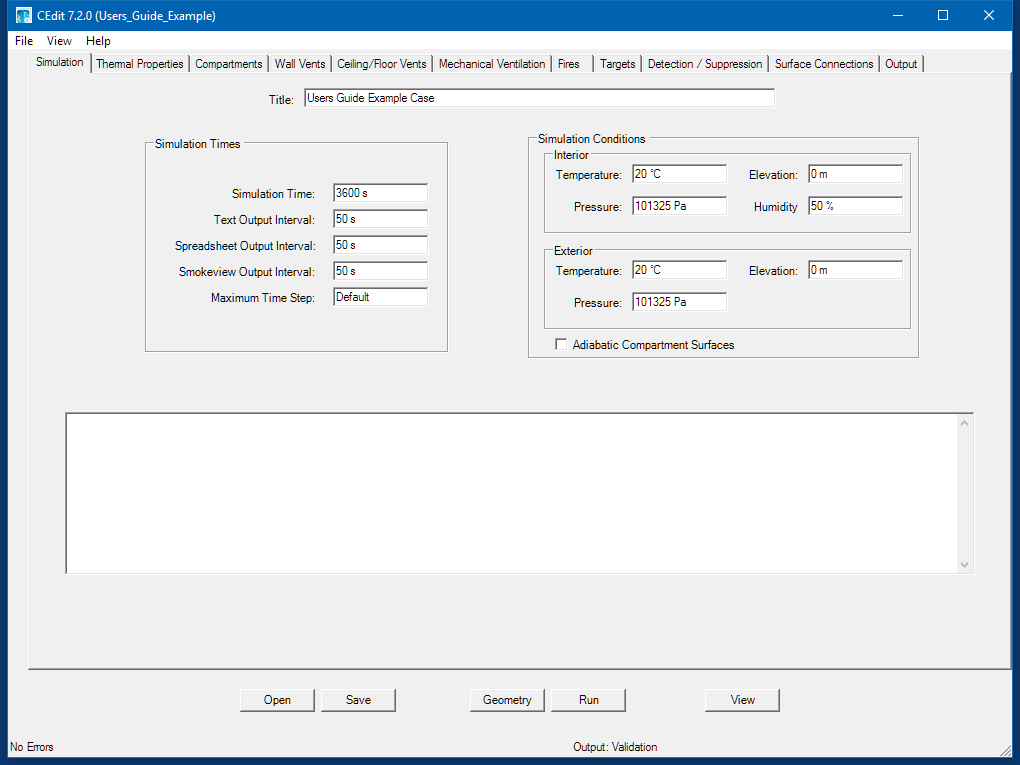
\includegraphics[width=6.5in]{FIGURES/Environment_Tab}
\caption[The Primary CFAST Input Page]{The Primary CFAST Input Page.}
\label{primary_screen}
\label{Figure 1.1}
\end{figure}
The simple test case can be run from the program menu by clicking on the ``Run'' icon. The case should finish in a few seconds. To verify that the installation has been done correctly, the output of the model should appear as shown in Fig.~\ref{Run_Model}.
\begin{figure}[h!]
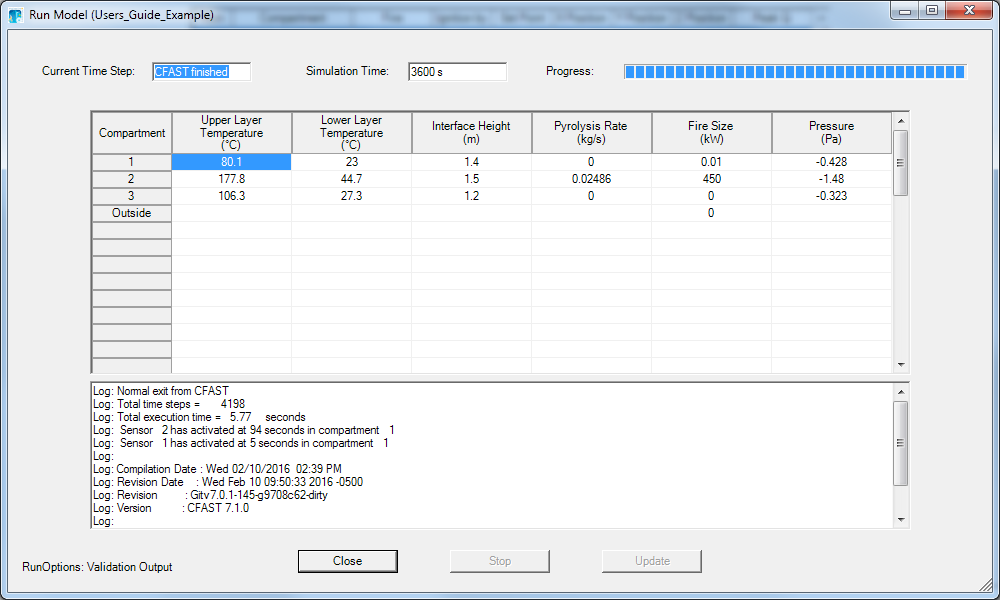
\includegraphics[width=6.5in]{FIGURES/Standard_Output}
\caption[The Standard CFAST Output Screen]{The Standard CFAST Output Screen.}
\label{Run_Model}
\end{figure}


\section{Basic Features}

The input parameters are organized via tabs near the top of the CEdit screen, as shown in Fig.~\ref{primary_screen}.
\begin{description}
\item[Simulation Environment] includes simulation time, specification of model outputs, and ambient conditions. Also included on the page are a constantly updated list of errors, warnings, and messages about the input file specification or model simulation.
\item[Thermal Properties] defines the thermal conductivity, specific heat, density, thickness and emissivity values for all materials and fuel sources to be used in a simulation.
\item[Compartments] defines the size, construction characteristics, and position of the compartments in a simulation.
\item[Wall Vents] define doors and windows.
\item[Ceiling/Floor Vents] define holes in the ceiling/floor.
\item[Mechanical Ventilation] defines forced air ventilation.
\item[Fires] include user specification of the initial fire source and any additional burning objects in one or more of the compartments of the simulation.
\item[Targets] provide the ability to calculate the temperature and net heat flux to objects placed and oriented arbitrarily in the structure.
\item[Detection / Suppression] defines any heat alarms and sprinklers in the compartments of the simulation.
\item[Surface Connections] allows for more detailed description of the connections between compartments in the simulation to better simulate the transfer of heat from compartment to compartment in the simulation.
\item[Visualizations] allows specification of one or more 2-D and 3-D visualizations to be added to the simulation for viewing with Smokeview. Note that these can require significant additional computational time than a basic CFAST simulation without visualizations.
\end{description}


\section{The View Menu}

The View menu allows you to view or print the input data file, output file (if the simulation has been run and a text output file generated) and the log file of the simulation. If one of the items does not exist on the user's hard disk, the selection is grayed out.
\begin{description}
\item[Select Engineering Units] allows you to select the units for input and output. By default, most outputs are in S.I. units, with temperature in Celsius.
\end{description}


\section{The Help Menu}

The Help menu accesses this user's guide, the CFAST web site, or an about dialog box that displays the user license and version of the program.





\chapter{Simulation Environment}

The Environment page defines the initial conditions and simulation time for the CFAST input file.

\begin{figure}[ht]
\centering
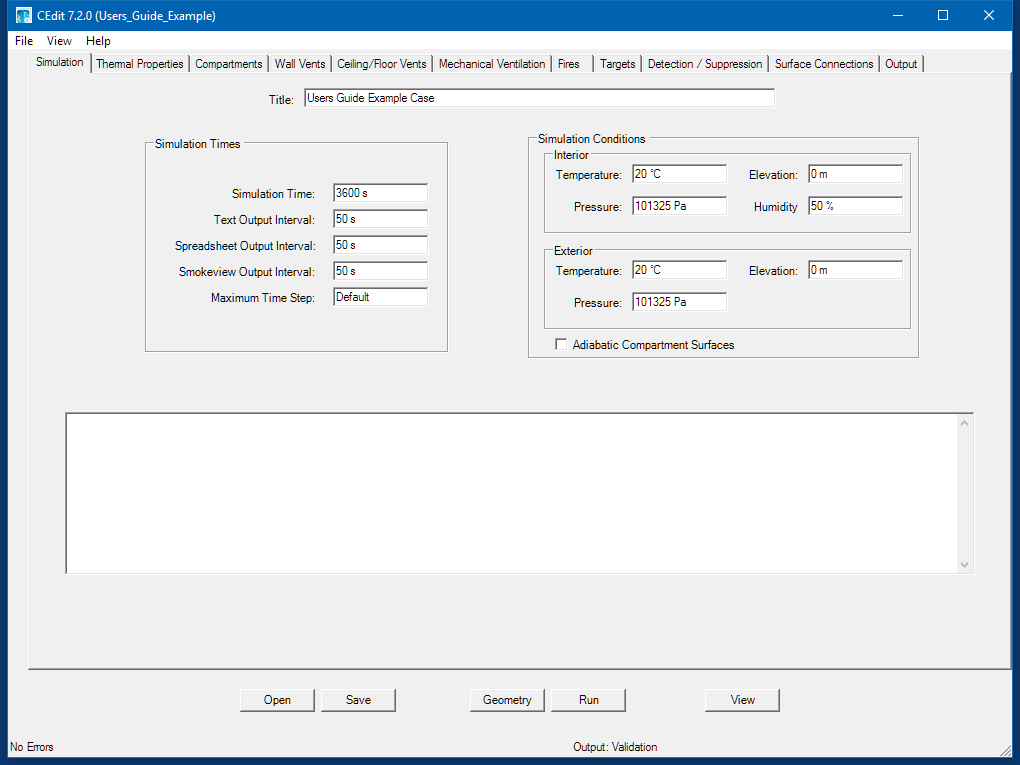
\includegraphics[width=6.5in]{FIGURES/Environment_Tab}
\caption[The CFAST Simulation Environment Tab]{The CFAST Simulation Environment Tab.}
\end{figure}

\section{Version and Title}
\label{info:HEAD}

\begin{description}
\item[Version] The version of CFAST being used by the user. Version number can be found in the upper left corner in the CEdit user interface as shown in Fig. \ref{Figure 1.1}.

\item[Title] The first thing to do when setting up an input file is to give the simulation a title. The title is optional and may consist of letters, numbers, and/or symbols and may be up to 50 characters. All output files will be tagged with this character string.
\end{description}




\section{Simulation Times}
\label{info:TIME}

\begin{description}
\item[Simulation Time] (default units: s, default value, 900 s): The length of time over which the simulation takes place. The maximum value for this input is 86400 s (1 day).

\item[Text Output Interval] (default units: s, default value, 60 s): The time interval between each printing of the output data.  If equal to zero, no output values will appear.

\item[Spreadsheet Output Interval] (default units: s, default value, 15 s): CFAST can output the results of the simulation in a set of comma-delimited spreadsheet files. This parameter defines the time interval between these outputs. A value greater than zero must be used if the spreadsheet files are desired.

\item[Smokeview Output Interval] (default units: s, default value: 15 s): CFAST can output a subset of the results in a format compatible with the visualization program Smokeview. This input defines the time interval between outputs of the model results in a Smokeview-compatible format.  A value greater than zero must be used if the Smokeview output is desired.

\item[Maximum Time Step] (default units: s, default value: 2 s): CFAST will automatically adjust the time interval for the solution of the differential equation set up or down so that the simulation is as efficient as possible within the pre-defined error tolerances. This parameter places a maximum value for the equation solver and can normally be left at the default value. In cases (which are hopefully rare) where the model fails to converge on a solution, this value can be reduced which often will allow the simulation to successfully complete.
\end{description}




\section{Simulation Conditions}
\label{info:INIT}

Ambient conditions define the environment at which the scenario begins. Initial pressures in a structure are calculated simply as a lapse rate (related to the height above sea level) based on the NOAA/NASA tables \cite{GPO:Atmosphere}. It is convenient to choose the base of a structure to be at zero height and then reference the height of the structure with respect to that height.  The temperature and pressure must then be measured at that position.  Another possible choice would be the pressure and temperature at sea level, with the structure elevations then given with respect to mean sea level.  This is also acceptable, but somewhat more tedious in specifying the construction of a structure.  Either of these choices works though, so long as they are consistent. Usually, the station elevation is set to zero and the pressure to ambient. The effect of changing these values is minor. Note that the equations implemented in the model are not designed to handle negative elevations and altitudes.

\begin{description}
\item[Temperature] (default units: \degc, default value: 20 \degc): Initial ambient temperature inside the structure at the station elevation.

\item[Humidity] (default units \% RH, default value: 50 \%): The initial relative humidity in the system, only specified for the interior.  This is converted to kilograms of water per cubic meter as an initial condition for both the interior and exterior of the structure.

\item[Temperature] (default units: \degc, default value: 20 \degc): Initial ambient temperature outside the structure at the station elevation.

\item[Pressure] (default units: Pa, default value: 101325 Pa): Initial values for ambient atmospheric pressure inside and outside the structure at the station elevation. The default value is standard atmospheric pressure at sea level.
\end{description}


\section{Miscellaneous}
\label{info:MISC}

Keywords associated to global parameters are organized in the miscellaneous namelist group.

\begin{description}
\item[Adiabatic Compartment Surfaces] When this box is checked, all of the compartment surfaces are assumed to be perfect insulators and the materials section of the compartments tab becomes grayed out. This feature is useful when designing an experiment in which it is safe to assume that there is no heat transfer to the walls of the compartments.

\item[Lower Oxygen Limit] (default units: \%, default value: 15~\%):  In the CFAST model, a limit is incorporated by limiting the burning rate as the oxygen level decreases until a ``lower oxygen limit'' (LOL) is reached. The lower oxygen limit is incorporated through a smooth decrease in the burning rate near the limit. Normally, this value would not be changed by the user.
\end{description}





\chapter{Thermal Properties}

The thermophysical properites of materials used for compartment surfaces or targets are set in the Thermal Properties tab.

\begin{figure}[ht]
\centering
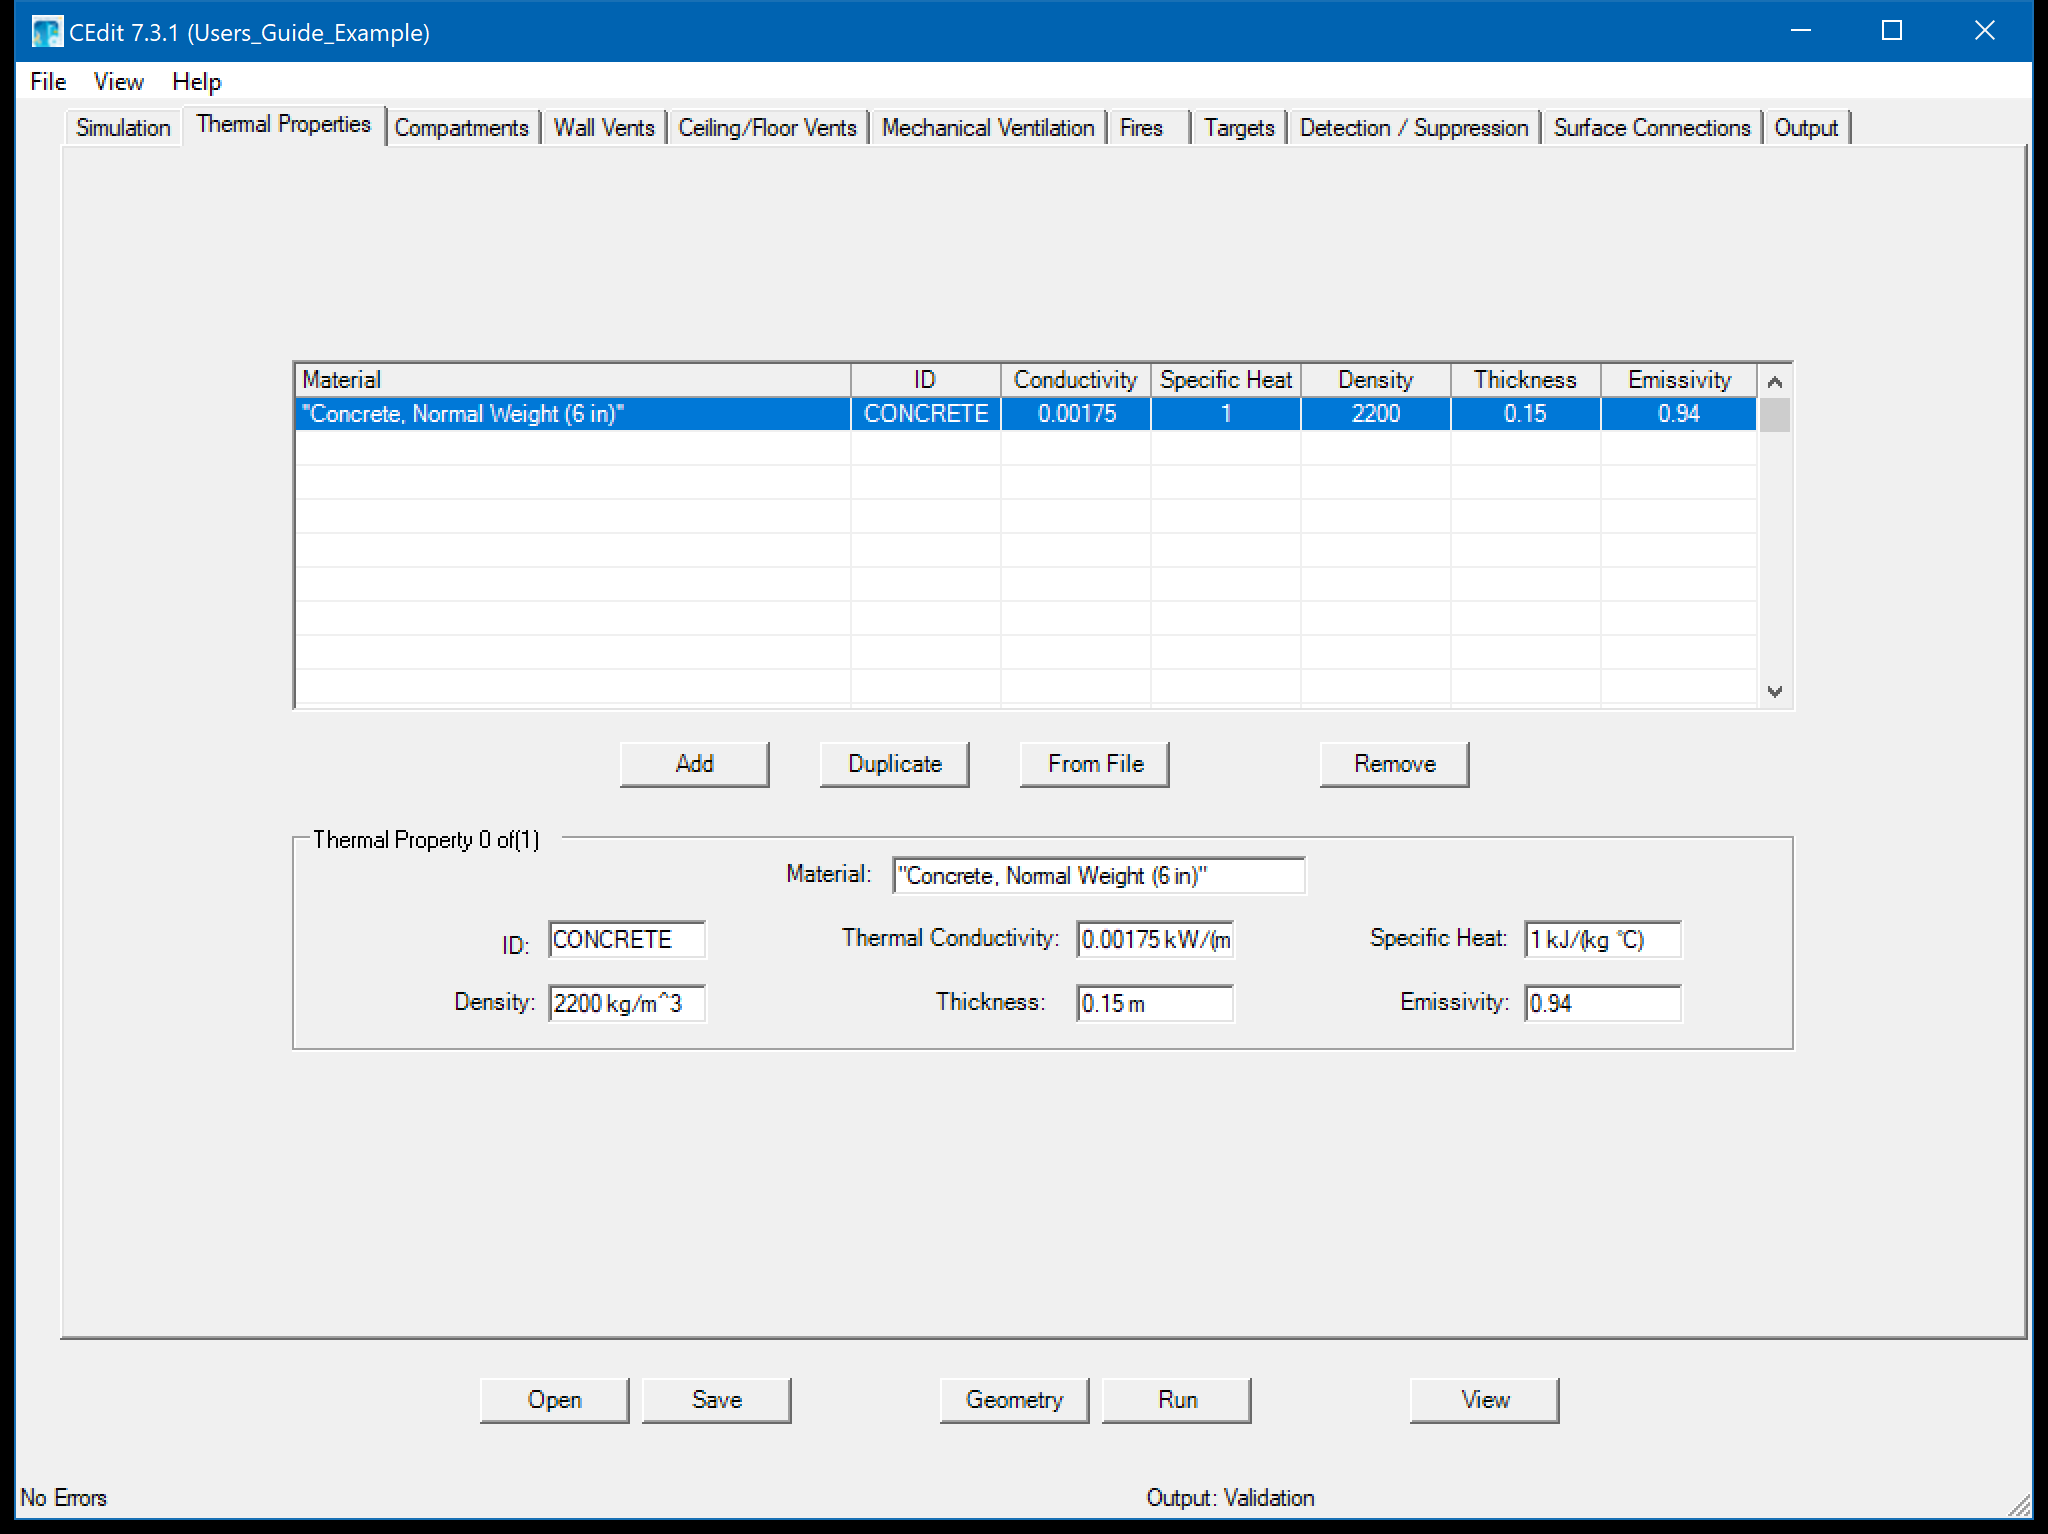
\includegraphics[width=6.5in]{FIGURES/Thermal_Properties_Tab}
\caption[The CFAST Thermal Properties Tab]{The CFAST Thermal Properties Tab.}
\end{figure}

\section{Adding Thermal Properties}
\label{info:MATL}

CFAST and CEdit do not include predefined thermal properties for compartment materials. Thus, the user needs to define materials for use within a specific simulation. These may be from other simulations or input directly from reference sources or test results. Clicking the `Add' button and assigning values to the following list of properties will create a set of thermal properties associated with a material used in a compartment or a target. The thermophysical properties are specified at one condition of temperature, humidity, etc.  Only a single layer per boundary is allowed (some previous versions allowed up to three).

\begin{description}
\item[Material] A descriptive name for the material.

%% Do we want to change the requirements on the ID. We don't have those requirements in the Name List
\item[ID] A one-word (no more than 8 characters) \textbf{unique} identifier for the material.  This identifier should not contain any spaces and is used in other CFAST inputs to identify the particular material referenced.

\item[Conductivity] (default units: kW/(m$\cdot$\degc)  or  kW/(m$\cdot$K)): Thermal conductivity for the material.

\item[Specific Heat] (default units: kJ/(kg$\cdot$\degc) or kJ/(kg$\cdot$K)): Specific heat for the material.

\item[Density] (default units: kg/m$^3$): Density for the material.

\item[Thickness] (default units: m): Thickness of the material.  Note that if two materials with identical thermal properties but with different thicknesses are desired, two separate materials must be defined.

\item[Emissivity] (default units: none, default value: 0.9): Emissivity of the material surface.  This is the fraction of radiation that is absorbed by the material.
\end{description}




\section{Adding Thermal Properties From Another File}

The `From File' button allows you to insert thermal properties from existing CFAST input files to the current simulation.

\begin{figure}[h!]
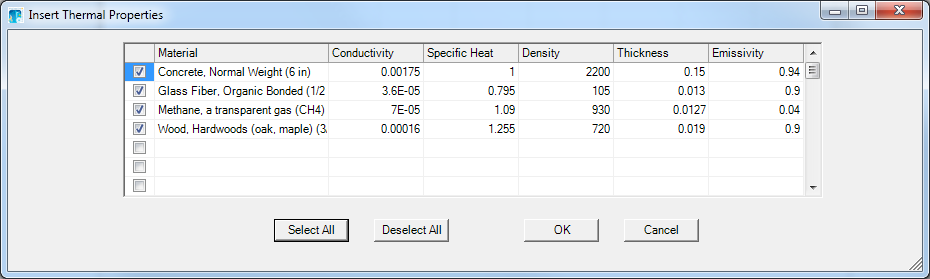
\includegraphics[width=6.5in]{FIGURES/Insert_Thermal_Properties}
\caption[Inserting Thermal Properties in CFAST]{Inserting Thermal Properties in CFAST.}
\end{figure}





\chapter{Compartments}
\begin{figure}[h!]
\begin{center}
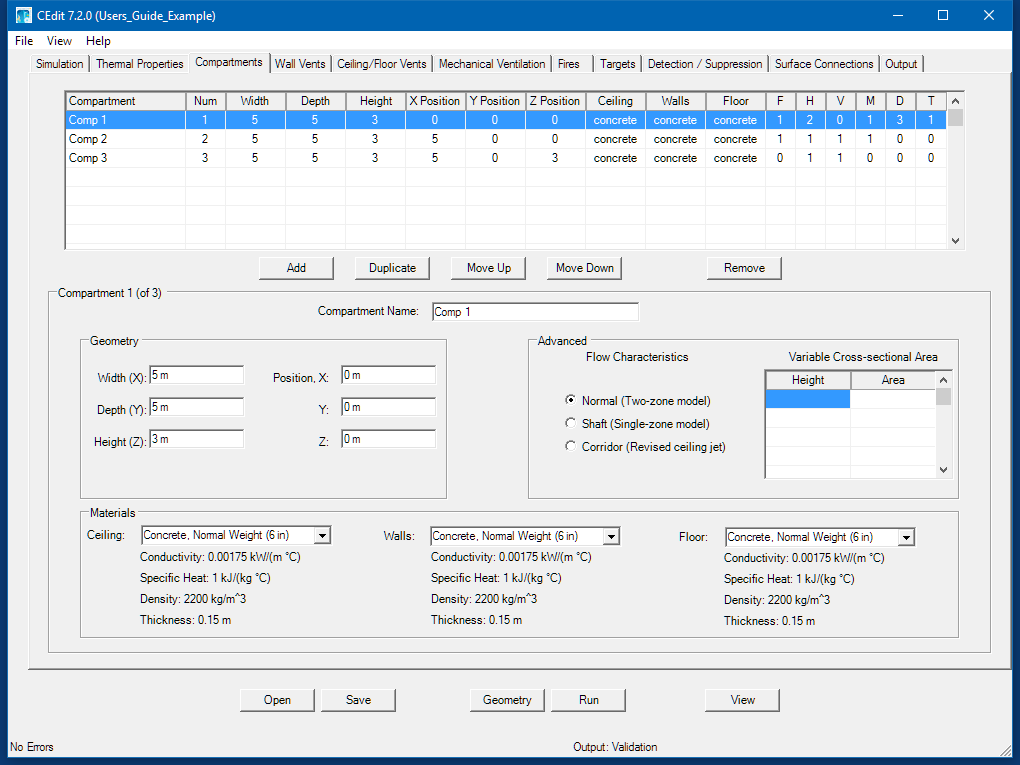
\includegraphics[width=6.5in]{FIGURES/Compartment_Geometry_Tab}
\caption[The CFAST Compartments Tab]{The CFAST Compartments Tab.}
\end{center}
\end{figure}

The Compartments page defines the size, position, materials of construction, and flow characteristics for the compartments in the simulation. Initially, only the simulation environment page and the 'Add' button on the compartment geometry and thermal properties pages are enabled; all other pages are not available to the user for detailed inputs until a compartment has been added to the simulation.

In order to model a fire scenario, the size and position of each compartment relavent to the scenario must be specified. For a compartment, the width, depth, compartment height and height of the floor of the compartment provide this specification. The maximum number of compartments for version 7 is 100. The usual assumption is that compartments are rectangular parallelepipeds. However, the CFAST model can accommodate odd shapes as equivalent floor area parallelepipeds or with a cross-sectional area that varies with height.

\begin{figure}[h!]
\begin{tabular*}{\textwidth}{c@{\extracolsep{\fill}}c}
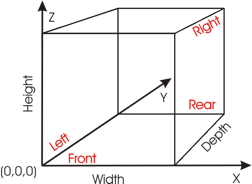
\includegraphics[width=2.5in]{FIGURES/CFAST_Coordinates} &
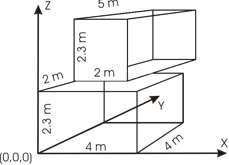
\includegraphics[width=2.6in]{FIGURES/CFAST_Absolute_Positioning} \\
Compartment Size & Compartment Position
\end{tabular*}
\caption[Compartment Orientation and Positioning in CFAST]{Compartment Orientation and Positioning in CFAST.}
\label{fig:compartment_positioning}
\end{figure}

In CEdit the default size of a room has width of 3.6 m, depth of 2.4 m, and height of 2.4 m. There are defaults for absolute positioning (0,0,0). All surfaces, i.e., the ceiling, walls and floor, are turned off by default. The fully mixed (single zone) and corridor models are turned off by default.

\label{Compartment_Geometry}Compartments in CFAST are most typically defined by a width, depth, and height.  If desired, compartments can be prescribed by the cross-sectional area of the compartment as a function of height from floor to ceiling for other shapes. The absolute position of the compartment with respect to a single structure reference point can be defined to ease visualization or to allow exact placement of vents and surfaces relative to other compartments in a detailed calculation. This specification is important for positioning the compartments for visualization in Smokeview.

\begin{description}
\item[ ID:] Compartments are identified by a unique alphanumeric name.  This may be as simple as a single character or number, or a description of the compartment.
\end{description}




\section{Geometry}
\label{info:COMP}
\begin{description}
\item[Width] (default units m, default value 3.6 m) specifies the width of the compartment as measured on the X axis from the origin (0,0,0) of the compartment.

\item[Depth]  (default units m, default value 2.4 m) specifies the depth of the compartment as measured on the Y axis from the origin (0,0,0) of the compartment.

\item[Height] (default units m, default value 2.4 m)  specifies the height of the compartment as measured on the Z axis from the origin (0,0,0) of the compartment.

\item[Position X] (default units m, default value 0.0 m)  specifies the absolute x coordinate of the lower, left, front corner of the room. All absolute positions for all compartments must be greater than or equal to zero, i.e., negative numbers are not allowed for these inputs. Important in positioning the compartments for visualization in Smokeview.

\item[Position Y] (default units m, default value 0.0 m)  specifies the absolute y coordinate of the lower, left, front corner of the room. All absolute positions for all compartments must be greater than or equal to zero, i.e., negative numbers are not allowed for these inputs. Important in positioning the compartments for visualiz
ation in Smokeview.

\item[Position Z] (default units m, default value 0.0 m)  specifies the height of the floor of each compartment with respect to station elevation specified by the internal ambient conditions reference height parameter.  The reference point must be the same for all elevations in the input data.  For example, the two rooms in the sample to the right in Fig.~\ref{fig:compartment_positioning} would be located at (0,0,0) and (0,2,2.3). All absolute positions for all compartments must be greater than or equal to zero, i.e., negative numbers are not allowed for these inputs.
\end{description}




\section{Materials}
\label{info:COMP2}
To calculate heat loss through the ceiling, walls, and floor of a compartment, the properties of the bounding surfaces must be known. This includes the thermophysical properties of the surfaces and the arrangement of adjacent compartments if inter-compartment heat transfer is to be calculated.
%In following paragraph is that supposed to be "convection" and not "conduction" or maybe "convection" should be added
The bounding surfaces are the ceilings, walls and floors that define a compartment. These are referred to as thermophysical boundaries, since each participates in conduction and radiation as well as defining the compartments, unless these phenomena are explicitly turned off.

The thermophysical properties of the materials to be used to define the surfaces are defined in the Thermal Propertied tab described in section \ref{info:MATL}. The materials are then assigned to the ceiling, wall, and floor surfaces by use of the material ID

\begin{description}
\item[Ceiling Material ID] (default value: Off): material name from the thermal properties from the Materials tab used for the ceiling surface of the compartment.

\item[Wall Material ID] (default value: Off): material name from the thermal properties from the Materials tab used for the wall surfaces of the compartment.

\item[Floor Material ID] (default value: Off): material name from the thermal properties from the Materials tab used for the floor surface of the compartment.
\end{description}

\graybox{
If the thermophysical properties of the enclosing surfaces are not included, CFAST will treat them as adiabatic (no heat transfer). \\

If a name is used which is not in the input file, the model should stop with an error message. \\

The back surfaces of compartments are assumed to be exposed to ambient conditions unless specifically specified (see the section on Surface Connections to specify heat transfer connections between compartments).
}




\section{Modeling a Compartment as a Tall Shaft or Long Corridor}
\label{info:COMP3}
For tall compartments or those removed from the room of fire origin, the compartment may be modeled as a single, well-mixed zone rather than the default two-zone assumption. A single zone approximation is appropriate for smoke flow far from a fire source, where the two-zone layer stratification is less pronounced than in compartments near the fire or in situations where the stratification does not occur. Examples are elevators, shafts, complex stairwells, or compartments far from the fire.

By specifying the compartment as a corridor, the ceiling jet temperature is calculated with a different empirical correlation that results in a somewhat higher temperature near the ceiling.  This will impact, for example, detectors, sprinkler, and targets near the ceiling in corridors.

\begin{description}
\item[Normal (Two-zone model)] Conditions in the compartment are calculated with the normal two-zone approach. This is the default model used for a compartment.

\item[Shaft (Single-zone model)] Conditions in the compartment are calculated as a single well-mixed zone.

\item[Corridor (Revised ceiling jet)] Conditions in the compartment are calculated with the normal two-zone approach. Ceiling jet temperatures in the compartment are calculated with a revised empirical correlation specific to corridors.
\end{description}




\section{Defining Variable Compartment Area}
\label{info:COMP4}
The Compartment Geometry page includes two additional entries that may be used for defining compartment properties for spaces which are not rectangular in area.  Values for a chosen compartment are entered in a spreadsheet.
\begin{description}
\item[Height Value(s)] (default units: m): Height off the floor of the compartment.
\item[Area Value(s)] (default units m$^2$): Cross-sectional area at the corresponding Height.
\end{description}

Once the total compartment volume is determined from the set of cross-sectional area and height inputs, an effective width and depth are calculated (maintaining the original user input for compartment height) so the compartment volume matches the actual total volume of the compartment. The aspect ratio (width/depth) is maintained.

Cross-sectional area values should be input in order by ascending height. If the first height value is not zero (i.e., at floor level), the cross-sectional area is assumed constant from the floor to the height specified in the first cross-sectional area value.
% Isn't the highest value by definition the ceiling hieght? Should that paragraph go away?
Similarly, if the last height value is not at the ceiling height, the cross-sectional area is assumed constant from the height specified in the last cross-sectional area value to the ceiling. Between any two adjacent cross-sectional area data values in the input list, the area is assumed to be a pyramidal section (which by definition maintains the same width to depth aspect ratio for the compartment from floor to ceiling).

CFAST uses the variable cross-sectional area inputs to determine the layer height. The equations solved by CFAST determine the volume of the upper layer. For a normal rectangular room, this corresponds directly to a layer height. For a variable cross-sectional area compartment, a numerical integration of the area inputs beginning at the ceiling is used to determine the height at which the upper layer occupies the calculated volume of the upper layer.




\section{Modeling Compartment Leakage}
\label{info:COMP5}
CFAST can automatically calculate leakage between one or more compartments and the outdoors. Leakage is specified for each desired compartment as a leakage area per unit wall area and/or per unit floor area.

\begin{description}
\item[Wall Leakage] (default units: m$^2$/m$^2$): Leakage area ratio input as the leakage are per unit wall area.
\item[Floor Leakage] (default units: m$^2$/m$^2$): Leakage area ratio input as the leakage are per unit floor area.
\end {description}

For reference, the following table is taken from the \textit{Handbook of Smoke Control Engineering} \cite{Klote:2012}.

\begin{table}[ht]
\begin{center}
\caption{Sample Flow Area of Walls and Floors of Commercial Buildings from the \textit{Handbook of Smoke Control Engineering} \cite{Klote:2012}, used with persmission}
\label{tbl:leakageareas}
\begingroup
\renewcommand{\arraystretch}{1.2}
\begin{tabular}{|l|c|c|}
\hline
Construction Element   & Leakage                        & \shortstack{Leakage Area (m$^2$/m$^2$) \\ Leakage Area per Unit Wall Area}   \\ \hline
\multirow{4}{*}{\shortstack[l]{\textbf{Exterior building walls} \\ \\ {\small (includes construction cracks} \\ {\small and cracks around windows and doors)}}}             & Tight      & $5.0 \times 10^{-5}$   \\
                                                                                                                                                                      & Average    & $1.7 \times 10^{-4}$ \\
                                                                                                                                                                      & Loose      & $3.5 \times 10^{-4}$ \\
                                                                                                                                                                      & Very Loose & $1.2 \times 10^{-3}$ \\ \hline

\multirow{3}{*}{\shortstack[l]{\textbf{Stairwell walls} \\ \\ {\small (includes construction cracks but} \\ {\small not cracks around windows and doors)}}}                & Tight      & $1.4 \times 10^{-5}$   \\
                                                                                                                                                                      & Average    & $1.1 \times 10^{-4}$ \\
                                                                                                                                                                      & Loose      & $3.5 \times 10^{-4}$ \\ \hline

\multirow{3}{*}{\shortstack[l]{\textbf{Elevator shaft walls} \\ \\ {\small (includes construction cracks but} \\ {\small not cracks around doors)}}}                       & Tight      & $1.8 \times 10^{-4}$   \\
                                                                                                                                                                      & Average    & $8.4 \times 10^{-4}$ \\
                                                                                                                                                                      & Loose      & $1.8 \times 10^{-3}$ \\ \hline \hline
Construction Element   & Leakage                        & \shortstack{Leakage Area (m$^2$/m$^2$) \\ Leakage Area per Unit Floor Area}   \\ \hline

\multirow{3}{*}{\shortstack[l]{\textbf{Floors} \\ {\small (includes construction cracks and} \\ {\small gaps around penetrations)}}}                                    & Tight      & $6.6 \times 10^{-6}$   \\
                                                                                                                                                                      & Average    & $5.2 \times 10^{-5}$ \\
                                                                                                                                                                      & Loose      & $1.7 \times 10^{-4}$ \\ \hline

\end{tabular}
\endgroup
\end{center}
\end{table}



\chapter{Vents}
\section{Natural Ventilation}

%% Do we want to be more technically correct in our definition?  E.g., two compartments not directly connected to each other by a vent but both connected to a third compartment are not
%% isolated from each other but they are remote from each other. Do we care?
Natural ventilation can occur when two compartments are connected via open doorways or windows (\textbf{Wall Vents}); or when two compartments are connected via \textbf{Floor/Ceiling Vents}. If no vents are specified between two compartments, they are assumed to be isolated from each other.

\subsection{Wall Vents}
\label{info:VENT}
\begin{figure}[h!]
\begin{center}
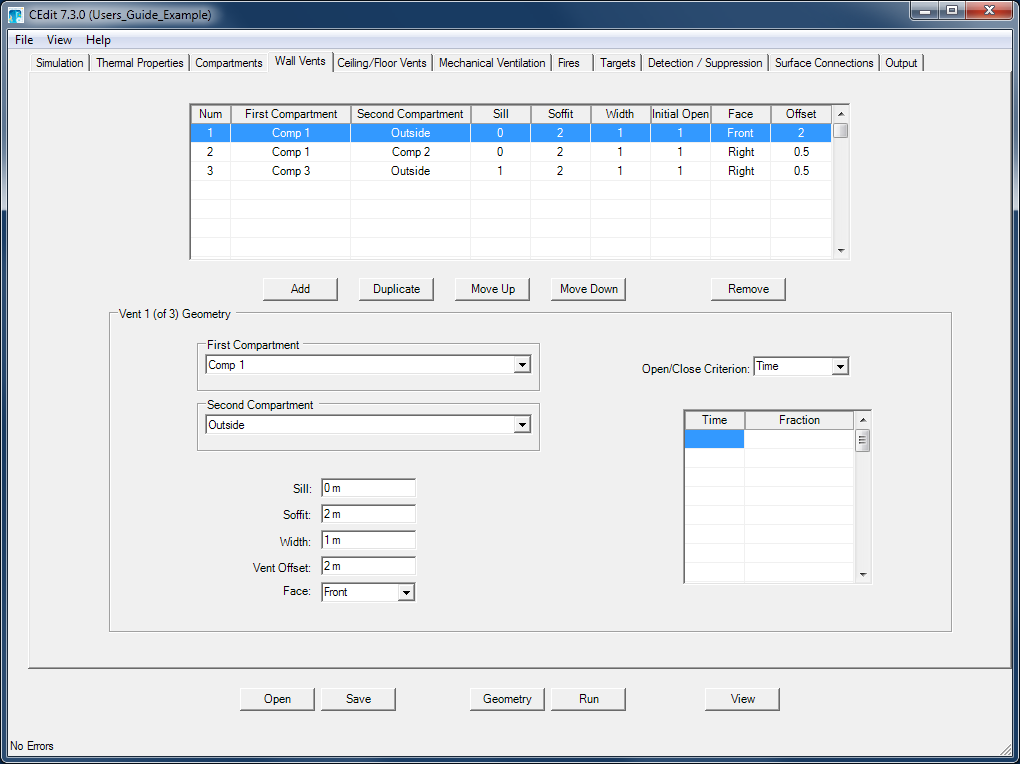
\includegraphics[width=6.5in]{FIGURES/Natural_Flow_Tab}
\caption[The CFAST Wall Vents Tab]{The CFAST Wall Vents Tab.}
\end{center}
\end{figure}

Wall vents are doors or windows that connect compartments that physically overlap in elevation, or that connect to the outside. Horizontal flow connections may also be used to account for leakage between compartments or to the outdoors.

\begin{description}
\item[ID] The selected name must be unique (i.e., not the same as another vent in the same simulation).
\item[First Compartment] First of the two compartments connected by a door or window. All specifications of the vent are made relative to the floor of the first compartment.
\item[Second Compartment] Second of the two compartments connected by a door or window.
\item[Sill] (default units: m, default value: 0 m): Height of the bottom of the opening relative to the floor of the first compartment.
\item[Soffit] (default units: m, default value: 0 m): Height of the top of the opening relative to the floor of the first compartment.
\item[Width] (default units: m, default value: 0 m): The width of the opening.
\item[Vent Offset] (default units: m, default value: 0 m): For visualization only, the horizontal distance between the near edge of the vent and the origin of the axis defined by the selected face (below) in the first compartment.
\item[Face] The wall on which the vent is positioned.  Choices are Front, Rear, Right, Left and are relative to the X-Z plane (Front and Rear faces are parallel to the X-axis; left and right are parallel to the Y-axis).
\end{description}

Vents in CFAST can be opened or closed at user-specified times or by a user-specified target's surface temperature or incident heat flux. For time-based opening changes, the inputs are a series of time points and associated opening fractions from 0 (fully closed) to 1 (fully open).

\begin{description}
\item[Time] (default units: s, default values: 0 s): Time during the simulation at which to begin or end a change in the open fraction.
\item[Fraction] (default value: 1, fully open): Fraction between 0 and 1 of the vent width to indicate the vent is closed, partially-open, or fully-open as the associated time point.
\end{description}

For condition-based opening changes, the inputs specify an associated target, trigger value, and vent opening fractions before and after the trigger value has been reached.

\begin{description}
\item[Open/Close Criterion] The time of ignition can be controlled by a user-specified time, or by a user-specified target's surface temperature or incident heat flux.
\item[Set Point] The critical value at which the vent opening change will occur. If it is less than or equal to zero, the default value of zero is taken.
\item[Trigger Target] User-specified target used to calculate surface temperature or incident heat flux to trigger a vent opening change. Target placement is specified by the user as part of the associated target definition.
\item[Pre-Activation Fraction] (default value: 1, fully open): Fraction between 0 and 1 of the vent width to indicate the vent is partially open at the start of the simulation.
\item[Post-Activation Fraction] (default value: 1, fully open): Opening fraction at the end of the simulation. The transition from the pre-activation fraction to the post-activation value is assumed to occur over one second beginning when the specified set point value is reached.
\end{description}

\graybox{CFAST assumes a linear transition between time points. If the initial time specified for a time-changing opening fraction is non-zero, the vent is assumed to be open at the initial value of the open fraction from the beginning of the simulation up to and including the time associated with the initial value of the opening fraction. If the final value of the opening fraction is less than the total simulation time, the vent is assumed to be open at the final value of the opening fraction from and including the time associated with the final value of the opening fraction until the end of the simulation.}




\subsection{Ceiling/Floor Vents}
\label{info:VENT2}
\begin{figure}[h!]
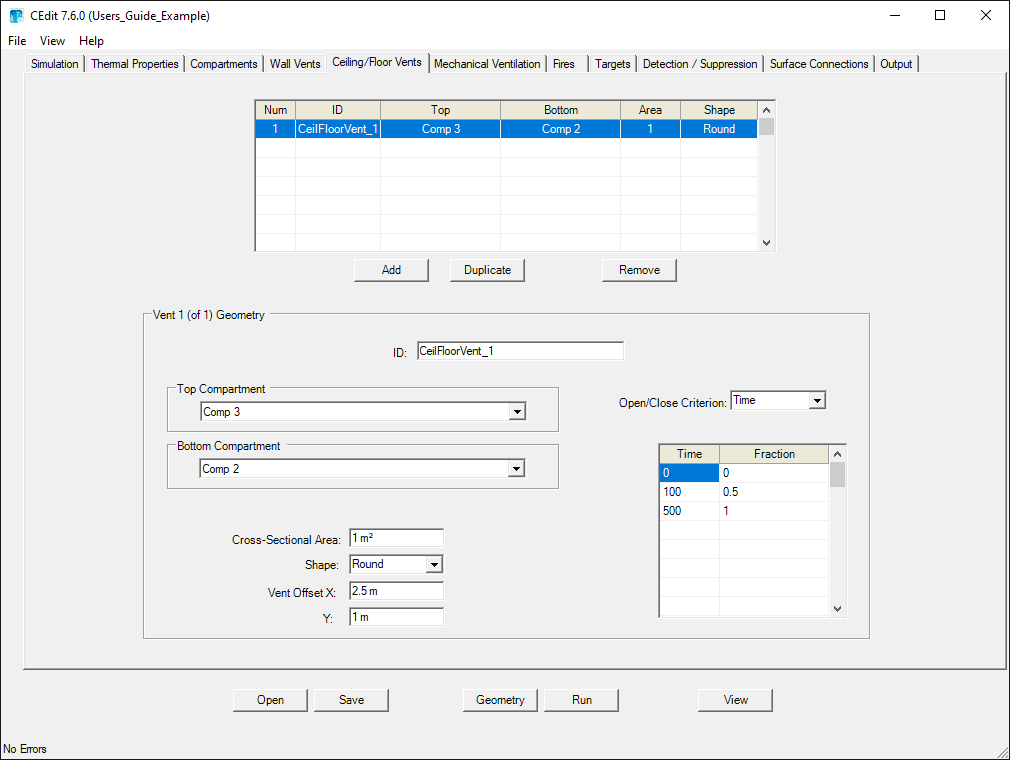
\includegraphics[width=6.5in]{FIGURES/Vertical_Flow_Tab}
\caption[The CFAST Ceiling/Floor Vents Tab]{The CFAST Ceiling/Floor Vents Tab.}
\end{figure}

Examples of these openings are scuddles in a ship, or a hole in the roof of a residence. Connections can exist between compartments or between a compartment and the outdoors. Combined buoyancy and pressure-driven flow through a vertical flow vent is possible when the connected spaces adjacent to the vent are filled with gases of different density in an unstable configuration, with the density of the top space greater than that of the bottom space. With a moderate cross-vent pressure difference, the instability leads to a bi-directional flow between the two spaces. For relatively large cross-vent pressure difference the flow through the vent is unidirectional.

\begin{description}
\item[ID] The selected name must be unique (i.e., not the same as another vent in the same simulation).
\item[Top Compartment] Compartment where the vent is in the floor
\item[Bottom Compartment] The adjacent compartment where the vent is in the ceiling.
\label{Ceil Cross-sectional Area}
\item[Cross-sectional Area] (default units: m$^2$, default value: 0 m$^2$)
\label{Ceil Shape}
\item[Shape] The shape factor changes the calculation of the effective diameter of the vent and flow coefficients for flow through the vent.
\item[Vent Offset] (default units: m, default value: 0 m): For visualization only, the horizontal distances between the center of the vent and the origin of the X and Y axes in the upper compartment. See figure \ref{fig:compartment_positioning} for axis position conventions in CFAST.
\end{description}

Vents in CFAST can be opened or closed at user-specified times or by a user-specified target's surface temperature or incident heat flux. For time-based opening changes, the inputs are a series of time points and associated opening fractions from 0 (fully closed) to 1 (fully open).

\begin{description}
\item[Time] (default units: s, default value: 0 s): Time during the simulation at which to begin or end a change in the open fraction.
\item[Fraction] (default value: 1, fully open): Fraction between 0 and 1 of the vent width to indicate the vent is closed, partially-open, or fully-open as the associated time point.
\end{description}

For condition-based opening changes, the inputs specify an associated target, trigger value, and vent opening fractions before and after the trigger value has been reached.

\begin{description}
\item[Open/Close Criterion] The time of ignition can be controlled by a user-specified time, or by a user-specified target's surface temperature or incident heat flux.
\item[Set Point] The critical value at which the vent opening change will occur. If it is less than or equal to zero, the default value of zero is taken.
\item[Trigger Target] User-specified target used to calculate surface temperature or incident heat flux to trigger a vent opening change. Target placement is specified by the user as part of the associated target definition.
\item[Pre-Activation Fraction] (default value: 1, fully open): Fraction between 0 and 1 of the vent width to indicate the vent is partially open at the start of the simulation.
\item[Post-Activation Fraction] (default value: 1, fully open): Opening fraction at the end of the simulation. The transition from the pre-activation fraction to the post-activation fraction is assumed to occur over one second beginning when the specified set point value is reached.
\end{description}

\graybox{CFAST assumes a linear transition between time points. If the initial time specified for a time-changing opening fraction is non-zero, the vent is assumed to be open at the initial value of the open fraction from the beginning of the simulation up to and including the time associated with the initial value of the opening fraction. If the final value of the opening fraction is less than the total simulation time, the vent is assumed to be open at the final value of the opening fraction from and including the time associated with the final value of the opening fraction until the end of the simulation.

CFAST allows only a single ceiling/floor connection between any pair of compartments included in a simulation because the empirical correlation governing the flow was developed using only a single opening between connected compartments.

Vertical connections can only be created between compartments that could be physically stacked based on specified floor and ceiling elevations for the compartments.  Some overlap between the absolute floor height of one compartment and the absolute ceiling height of another compartment is allowed.  However, whether the compartments are stacked or overlap somewhat, the ceiling/floor absolute elevations must be within 0.01 m of each other. The check is not done when the connection is to the outside.}




\section{Mechanical Ventilation}
\begin{figure}[h!]
\begin{center}
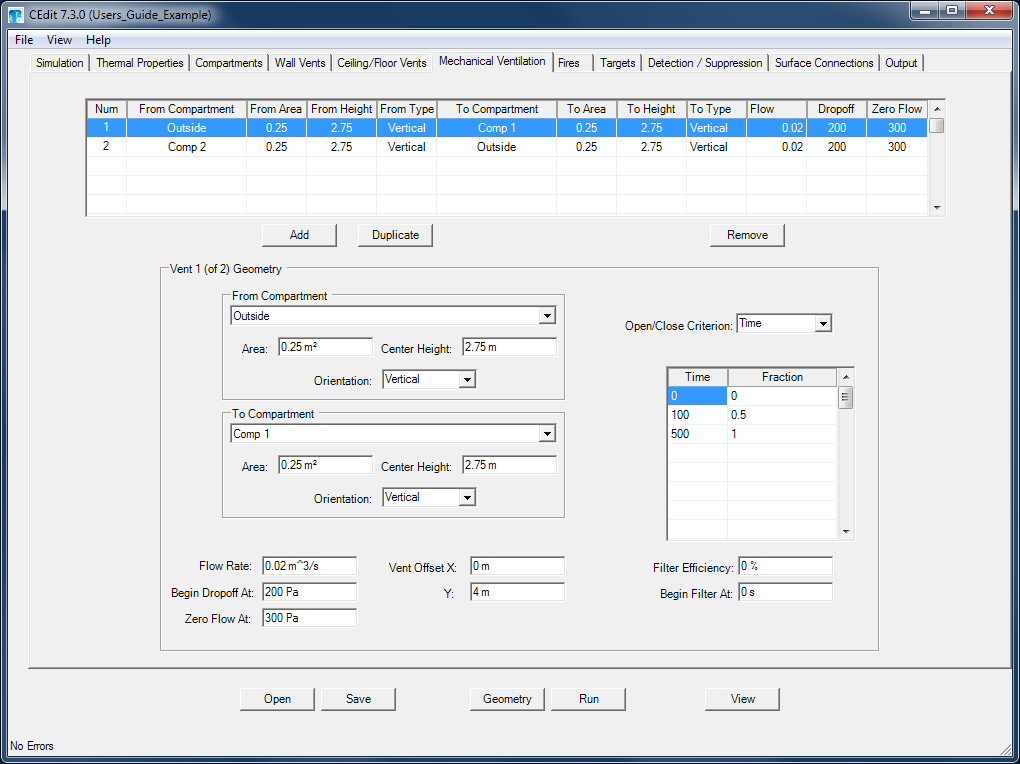
\includegraphics[width=6.5in]{FIGURES/Mechanical_Vent_Tab}
\caption[The CFAST Mechanical Vents Tab]{The CFAST Mechanical Vents Tab.}
\end{center}
\end{figure}

Fan-duct systems are commonly used in buildings for heating, ventilation, air conditioning, pressurization, and exhaust. Generally, systems that maintain comfortable conditions have either one or two fans.  Residences often have a system with a single fan. Further information about these systems is presented in  Klote and Milke \cite{Klote:2002} and the  \textit{Handbook of Smoke Control Engineering} \cite{Klote:2012}.

CFAST models mechanical ventilation in terms of user-specified volume flows at various points in the compartment. The model does not include duct work or fan curves, and thus mechanical ventilation connections are simply described by the connections to the two compartments and a fan whose throughput is a constant volumetric flow up to a user-specified pressure drop across the fan, dropping to zero at high backwards pressure on the fan.

\subsection{Connections to Compartments}
\label{info:VENT3}
\begin{description}
\item[ID]  The selected name must be unique (i.e., not the same as another mechanical ventilation system in the same simulation).
\item[First Compartment] The compartment from which the fan flow originates.
\item[Second Compartment] The compartment to which the fan flow terminates.
\item[Area] (default units: m$^2$, default value: 0 m$^2$): Cross-sectional area of the opening.
\label{Mech Height}
\item[Center Height] (default units: m, default value: 0 m): Height of the midpoint of the duct opening above the floor.
\item[Orientation] (default vertical) A horizontal diffuser implies vertical flow through the ceiling or floor of the compartment.  A vertical diffuser implies horizontal flow through a wall of the compartment.
\item[Vent Offset] (default units: m, Default value: 0 m): For visualization only, the horizontal distances between the center of the vent and the origin of the X and Y axes in the first compartment. See figure \ref{fig:compartment_positioning} for axis position conventions in CFAST.
\end{description}

Vents in CFAST can be opened or closed at user-specified times or by a user-specified target's surface temperature or incident heat flux. For time-based opening changes, the inputs are a series of time points and associated opening fractions from 0 (fully closed) to 1 (fully open).

\begin{description}
\item[Time] (default units: s, default values: 0 s): Time during the simulation at which to begin or end a change in the open fraction.
\item[Fraction] (default value: 1, fully open): Fraction between 0 and 1 of the vent width to indicate the vent is closed, partially-open, or fully-open as the associated time point.
\end{description}

\graybox{CFAST assumes a linear transition between time points. If the initial time specified for a time-changing opening fraction is non-zero, the vent is assumed to be open at the initial value of the open fraction from the beginning of the simulation up to and including the time associated with the initial value of the opening fraction. If the final value of the opening fraction is less than the total simulation time, the vent is assumed to be open at the final value of the opening fraction from and including the time associated with the final value of the opening fraction until the end of the simulation.}

For condition-based opening changes, the inputs specify an associated target, trigger value, and vent opening fractions before and after the trigger value has been reached.

\begin{description}
\item[Open/Close Criterion] The time of ignition can be controlled by a user-specified time, or by a user-specified target's surface temperature or incident heat flux.
\item[Set Point] The critical value at which the vent opening change will occur. If it is less than or equal to zero, the default value of zero is taken.
\item[Trigger Target] User-specified target used to calculate surface temperature or incident heat flux to trigger a vent opening change. Target is placement is specified by the user as part of the associated target definition.
\item[Pre-Activation Fraction] (default value: 1, fully open): Fraction between 0 and 1 of the vent width to indicate the vent is partially open at the start of the simulation.
\item[Post-Activation Fraction] (default value: 1, fully open): Opening fraction at the end of the simulation. The transition from the pre-activation fraction to the post-activation fraction is assumed to occur over one second beginning when the specified set point value is reached.
\end{description}




\subsection{Fans}
\label{info:VENT4}
CFAST does not include provisions for reverse flow through a fan, or a fan curve. Rather, you may specify a pressure above which the flow linearly decreases to zero.
\begin{description}
\label{Mech Flow Rate}
\item[Flow Rate] (default units: m$^3$/s, default value: 0 m$^3$/s): Constant flow rate of the fan.
\label{Mech Begin Drop Off Pressure}
\item[Begin Drop Off Pressure] (default units: Pa, default value: 200 Pa): Above this pressure, the flow begins a drop-off to zero. A hyperbolic tangent function is used to ensure a smooth transition from full flow at the ``Begin Drop Off Pressure'' to zero flow at the ``Zero Flow Pressure''.
\label{Mech Zero Flow Pressure}
\item[Zero Flow Pressure] (default units: Pa, default value: 300 Pa): The pressure above which the flow is zero.
\end{description}




\subsection{Filtering}
\label{info:VENT5}
For mechanical vents, there are two species that can be filtered out of the gas flow: soot and the user-defined trace species. Filters are applied only to fan openings. The fan must have been defined before the filter can be applied. Initially filtering is off.
\begin{description}
\label{Mech Filter Efficiency}
\item[Filter Efficiency] (default units:~\%, default value: 0\%): Flow through mechanical vents may include filtering that removes a user-specified portion of soot and trace species mass from the flow through the vent.  By default, there is no filtering applied; that is, all of the soot and trace species mass in the vent flow is passed through the vent. Within the user interface, this is specified as a filter efficiency of 0~\%.  If desired, you may specify the fraction of the soot and trace species mass to be removed as a percentage.
\label{Mech Begin Filtering At Time}
\item[Begin Filtering At Time] (default units: s, default value: 0 s): Time during the simulation at which the mechanical vent filtering begins.
\end{description}

\graybox{If the simulation includes mechanical ventilation filtering, care should be taken in choosing trace species production rates to insure the production rate is small compared to the total pyrolysis rate since the filtering removes mass from the system.  This will better allow appropriate conservation of mass in the solution of the system of differential equation.  For large production rates of trace species, scaling factors can be used (e.g., divide by 1000) for the trace species production rate to reduce the relative magnitude compared to the pyrolysis rate.  For analysis, the resulting trace species in compartments and filters can be converted back to original units multiplying by the scaling factor used.}






\chapter{Fires}
A fire in CFAST is specified via a time-dependent heat release rate (HRR). The specified heat of combustion is used to calculate the mass loss rate of fuel, from which the production rate of combustion products can be calculated using specified product yields. The heat release and the corresponding product generation rates go to zero when the lower oxygen limit is reached, and are replaced by the appropriate production rate of unburned fuel gas which is transported from zone to zone until there is sufficient oxygen and a high enough temperature to support combustion.

The model can simulate multiple fires in one or more compartments. These fires are treated as totally separate entities, with no interaction of the plumes. These fires can be ignited at a prescribed time, or when a corresponding target (see Chapter~\ref{chapter:targets}) reaches a specified temperature or heat flux.

The combustion model is defined by the following one-step reaction:
\begin{eqnarray}
   \mathrm{C_{n_\C}H_{n_H}O_{n_O}N_{n_N}Cl_{n_{Cl}}} &+&  \nu_\OTWO \, \mathrm{O_2}  \rightarrow  \nonumber \\[.1in]
   \nu_\COTWO \, \mathrm{CO_2} &+& \nu_\HTWOO \, \mathrm{H_2O} \; + \; \nu_\CO \, \mathrm{CO} \; + \; \nu_\So \, \mathrm{Soot} \; + \; \nu_\HCl \mathrm{HCl} \; + \; \nu_\HCN \mathrm{HCN} \label{stoich}
\end{eqnarray}
It is assumed that all the nitrogen and chlorine in the fuel are converted to HCN and HCl.

\begin{figure}[h!]
\begin{center}
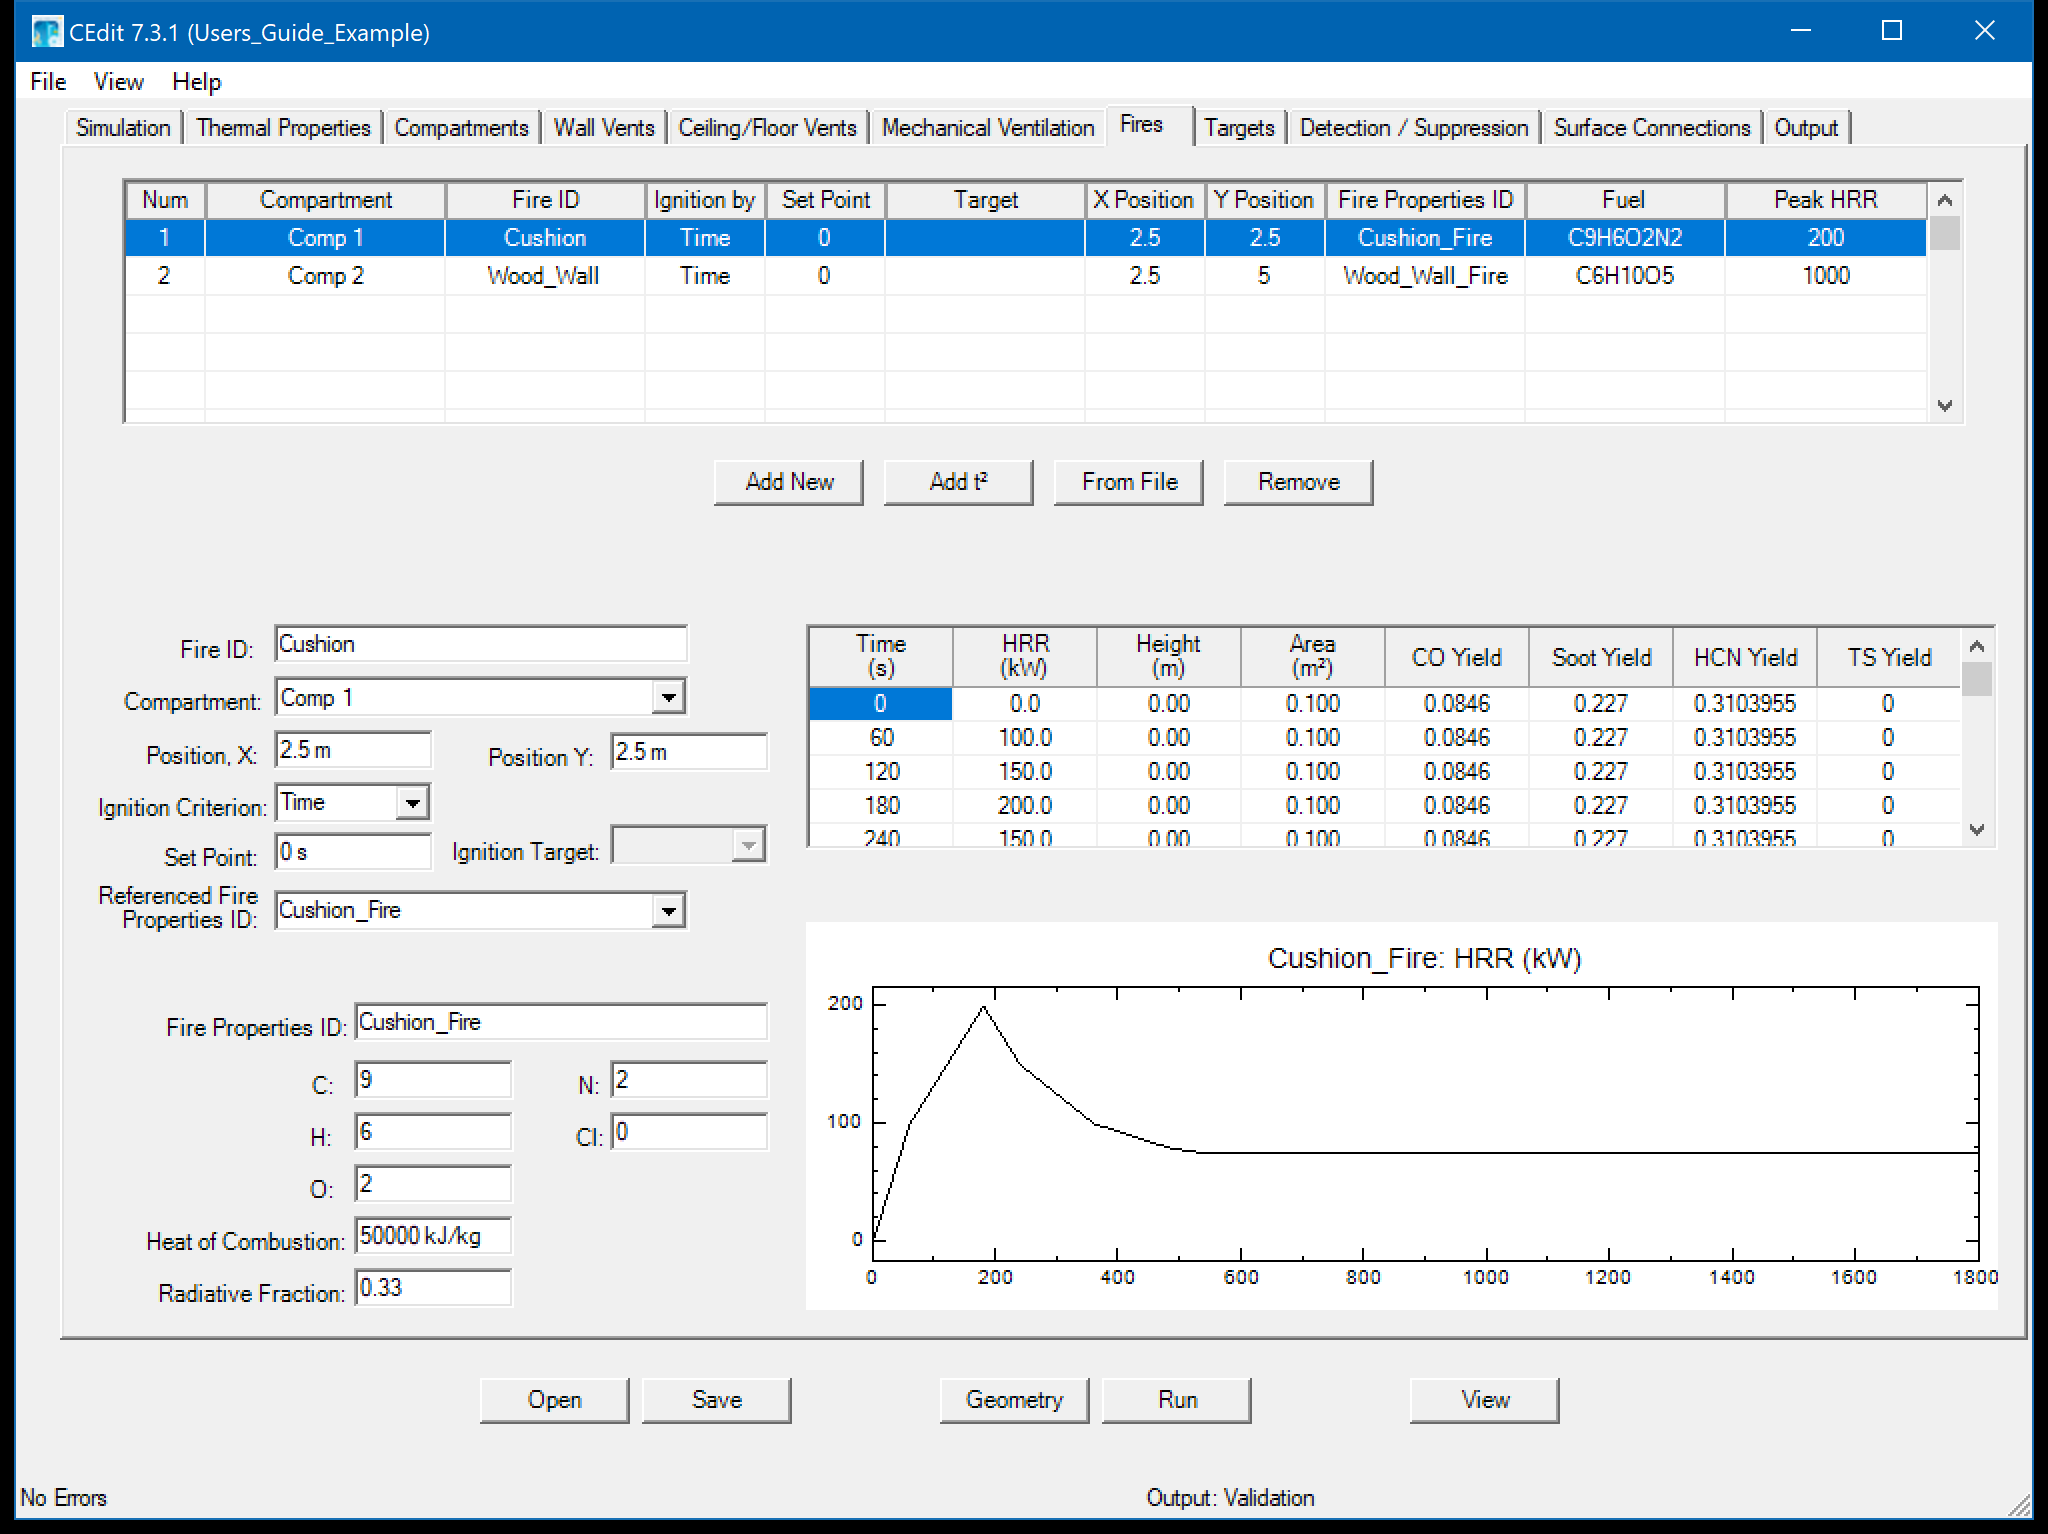
\includegraphics[width=6.5in]{FIGURES/Fire_Tab}
\caption[The CFAST Fires Tab]{The CFAST Fires Tab.}
\end{center}
\end{figure}


\section{Adding Fires}
\label{info:FIRE}
\label{sec:fire_inputs}
Fires in CFAST are defined in two parts: a ``Fire Definition'' that specifies the fuel composition, heat release rate, and species yields for the fire, and a ``Fire Instance'' that specifies the placement of a defined fire within a compartment in the simulation. A single fire definition may be associated with more than one fire instance in a simulation if desired.

For a new fire , click on the {\bf Add New} button or {\bf Add t$^2$} buttons within the fire definition block of inputs. The latter is useful because it has predefined quadratic growth rate options that are commonly used in fire analyses. See Section~\ref{tsq} for details. For each fire instance, specify the following properties:
\begin{description}
\item[Fire ID] The selected name must be unique (i.e., not the same as another fire instance in the same simulation).
\item[Compartment] Name of the compartment where the fire occurs.
\item[Position X, Y] (default units: m, default value: compartment center): Position of the center of the base of the fire relative to the front left corner of the compartment.
\item[Ignition Criterion] The time of ignition can be controlled by a user-specified time, or by a user-specified target's surface temperature or incident heat flux.
\item[Set Point] The critical value at which ignition will occur. If it is less than or equal to zero, the default value of zero is taken.
\item[Ignition Target] User-specified target used to calculate surface temperature or incident heat flux to ignite fire. Target is typically placed at the base of the fire to be ignited.
\item[Referenced Fire] the name of the associated fire definition for this fire instance can be selected from a list of fire definitions. A fire definition must exist before it can be selected.
\end{description}

Each instance of a fire can be unique fires with different chemical composition and time-dependent fire properties. Alternatively, two or more fires can reference the same set of fire properties. The following parameters define the composition and burning properties of the fire.
\begin{description}
\item[Fire Properties ID] The selected name must be unique (i.e., not the same as another fire definition in the same simulation). IDs for fire definitions can be the same as ones for fire instances.
\item[C, H, O, N, Cl] The number of each atom in the fuel molecule. Burning fuels in CFAST are assumed to be hydrocarbon fuels that contain at least carbon and hydrogen and optionally oxygen, nitrogen, and chlorine. All of the specified nitrogen and chlorine is assumed to completely react to form HCN and HCl.
\item[Heat of Combustion] (default units: kJ/kg, default value: 50000 kJ/kg): The energy released per unit mass of fuel consumed.
\item[Radiative Fraction] (default units: none, default value: 0.35): The fraction of the combustion energy that is emitted in the form of thermal radiation. Values for various fuels are suggested by Beyler~\cite{Beyler2:SFPE}.
\end{description}



\section{Time-Dependent Properties}
\label{info:FIRE2}
Following is a list of fire properties that can be specified as a function of time. The properties are linearly interpolated between specified points. If the simulation time is longer than the total duration of the fire, the final values specified for the fire are continued until the end of the simulation. Normal copy (Ctrl-C), cut (Ctrl-X), and paste (Ctrl-V) keyboard shortcuts work for data editing. In addition, Alt-Insert will insert a complete row above the currently-selected row in the spreadsheet and Alt-Delete will delete the current row in the spreadsheet.
\begin{description}
\item[Time] (default units: s, default values: none): Time from ignition.
\item[HRR] (default units: kW, default values: none): Heat release rate of the fire.
\item[Height] (default units: m, default values: 0 m): Height of the base of the fire.
\item[Area] (default units: m$^2$, default values: calculated from heat release rate such that the fire Froude number is unity\footnote{The Fire Froude Number, $\dot{Q}^*$, is defined as $\dot{Q}^* = \frac{\dot{Q}}{\rho_\infty c_p T_\infty \sqrt{gD} D^2}$. It is essentially the ratio of the fuel gas exit velocity and the buoyancy-induced plume velocity. Jet fires are characterized by large Froude numbers. Typical accidental fires have a Froude number near unity.}): Area of the base of the fire. The plume correlations used in CFAST generally regard the base to be circular. Do not set this value to zero because it is used in the various plume correlations.
\item[CO Yield] (default units: kg/kg, default value: 0 kg/kg): Mass of CO produced per unit mass of fuel consumed.
\item[Soot Yield] (default units: kg/kg, default value: 0 kg/kg): Mass of soot produced per unit mass of fuel consumed.
%Should this still be there if all the N2 in the fuel is assumed to go to HCN.
\item[HCN Yield] (default units: kg/kg, default value: 0 kg/kg): Mass of hydrogen cyanide produced per unit mass of fuel consumed.
\item[TS Yield] (default units: kg/kg, default value: 0 kg/kg): Mass of user-defined trace species per unit mass of fuel consumed. The trace species is transported along with the other products of combustion, but is assumed not to take part in the combustion reaction and is assumed not to be a significant source of overall mass for the system mass balance. This implies that the production rate of trace species specified should be small.
\end{description}


\section{Special Topic: t-Squared Fires}
\label{tsq}
Use the `Add t$^2$' button to create a new fire with a heat release rate that grows as a function of the time squared~\cite{Schifiliti:2002}:
\be
   \dQ(t) = \dQ_{\rm peak} \; \left( \frac{t}{t_{\rm peak}} \right)^2
\ee

\begin{figure}[h!]
\begin{center}
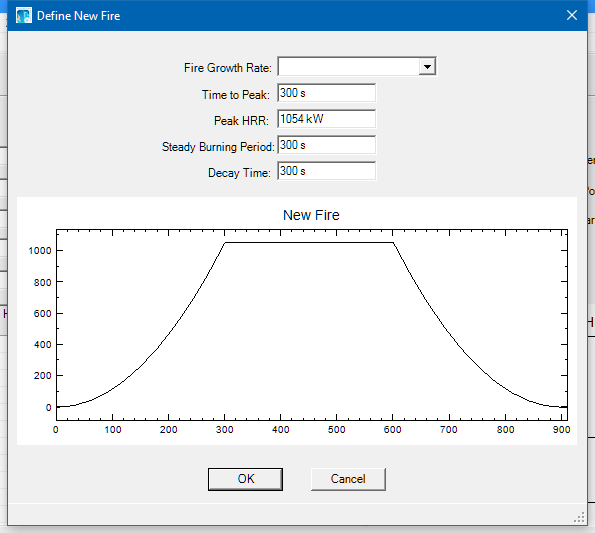
\includegraphics[width=5in]{FIGURES/Create_t2}
\caption[Inserting T-squared Fires in CFAST]{Inserting T-squared Fires in CFAST.}
\end{center}
\end{figure}

\begin{description}
\item[Fire Growth Rate] A set of specific t-squared fires labeled slow, medium, fast, or ultra-fast such that the fire reaches 1054~kW (1000~BTU/s) in 600~s, 300~s, 150~s, and 75~s.  A custom selection allows you to define any growth or decay rate desired.
\item[Time to Peak] (default units: s, default value: 300 s): The time for the fire to reach the peak HRR.
\item[Peak HRR] (default units: kW, default value: 1054 kW): The peak heat release rate of the t-squared fire.
\item[Steady Burning Period] (default units: s, default value: 300 s): Duration of time that the fire continues burning at the rate specified by the peak HRR.
\item[Decay Time] (default units: s, default value, 300 s): Duration of time for the fire to decay back to a zero value.  Decay follows the inverse of the t-squared growth rate.
\end{description}

%Where is the getting fire definitions from files?






\chapter{Measurement and Fire Protection Devices}
\label{info:DEVC}
\section{Targets}
\label{chapter:targets}

A target is any object in the simulation that can heat up via radiative and convective heat transfer. The heat conduction into the target is performed via a one-dimensional calculation in either cartesian or cylindrical coordinates.

\begin{figure}[h!]
\begin{center}
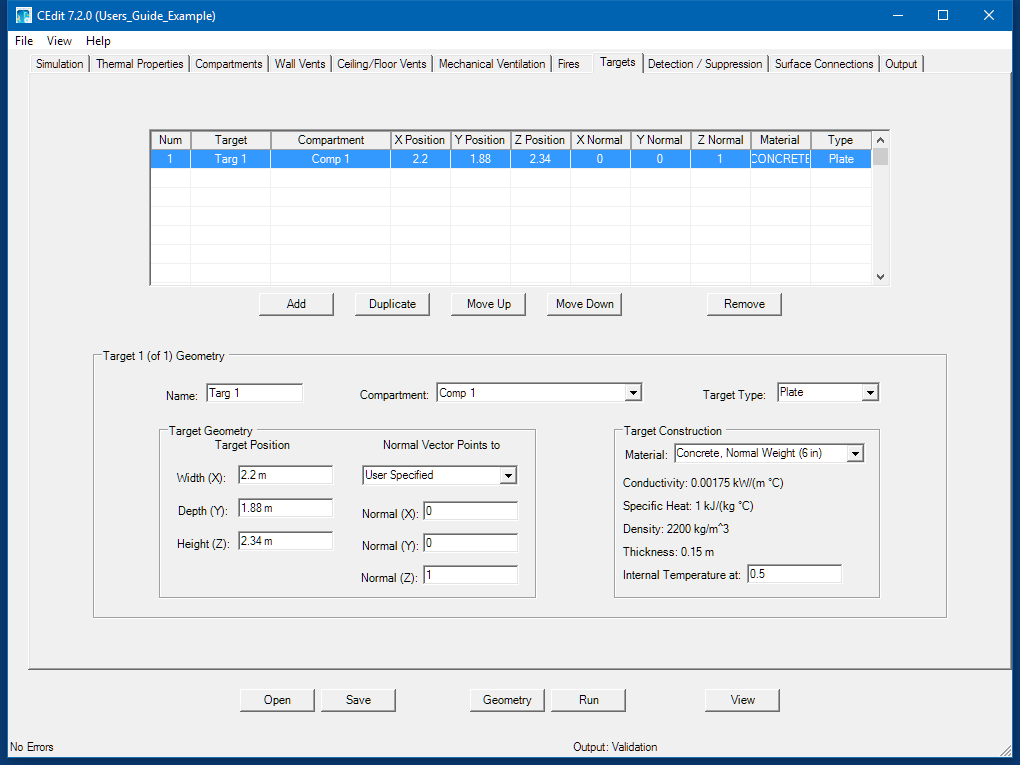
\includegraphics[width=6.5in]{FIGURES/Target_Tab}
\caption[The CFAST Targets Tab]{The CFAST Targets Tab.}
\end{center}
\end{figure}

\begin{description}
\item[ID] The selected name must be unique (i.e., not the same as another target in the same simulation).

\item[Compartment] The compartment in which the target is located.

\item[Target Type] Specify Plate, or Cylindrical.  For plate targets, CFAST solves a partial differential equation in cartesian coordinates, and for cylindrical targets, a partial differential equation in cylindrical coordinates.

\item[Width (X)] (default units: m): Distance from the left wall of the target compartment.

\item[Depth (Y)] (default units: m): Distance from the front wall of the target compartment.

\item[Height (Z)] (default units: m): Height of the target above the floor.

\item[Normal Vector (X,Y,Z)]: specifies a vector of unit length perpendicular to the exposed surface of the target. For example, the vector (-1,0,0) indicates that the target is facing the left wall. The vector (0,0,1) is facing the ceiling.

\item[Material] What the target is made of. Any existing material in the list of thermal properties may be used here. There can be only one material per target.

%What happens to interanl temperatrue when type is cylindrical
\item[Internal Temperature] (default units: none, default value: 0.5): For each target, CFAST calculates the internal temperature at a number of node points within the target. By default, the reported internal temperature (in the printed and spreadsheet output) is the temperature at the center of the target, e.g., equidistant from the front and back faces of the target. This input allows the user to override this default position. The input represents the position as a fraction of the thickness from the front surface to the back surface of the material.
\end{description}

\graybox{
If the target is only needed to report the local gas temperature, which may include the plume or ceiling jet, then you may specify arbitrary properties and normal vector. The output spreadsheet file includes the local gas temperature in addition to the target temperature.

The normal vectors in the $x$, $y$, and $z$ directions from a target at [$x$, $y$, $z$] to a location [$x_L$, $y_L$, $z_L$] are:
\begin{eqnarray}
x_N &=& \frac{x_L - x}{\sqrt{\brackets{x_L - x}^2 + \brackets{y_L - y}^2 + \brackets{z_L - z}^2}} \\[.1in]
y_N &=& \frac{y_L - y}{\sqrt{\brackets{x_L - x}^2 + \brackets{y_L - y}^2 + \brackets{z_L - z}^2}} \\[.1in]
z_N &=& \frac{z_L - z}{\sqrt{\brackets{x_L - x}^2 + \brackets{y_L - y}^2 + \brackets{z_L - z}^2}}
\end{eqnarray}
}




\section{Sprinklers and Detectors}
\label{info:DEVC2}
Sprinklers and detectors are both considered detection devices by the CFAST model and are handled using the same inputs.  Detection is based upon heat transfer to the detector. Fire suppression by a user-specified water spray begins once the associated detection device is activated.


\begin{figure}[h!]
\begin{center}
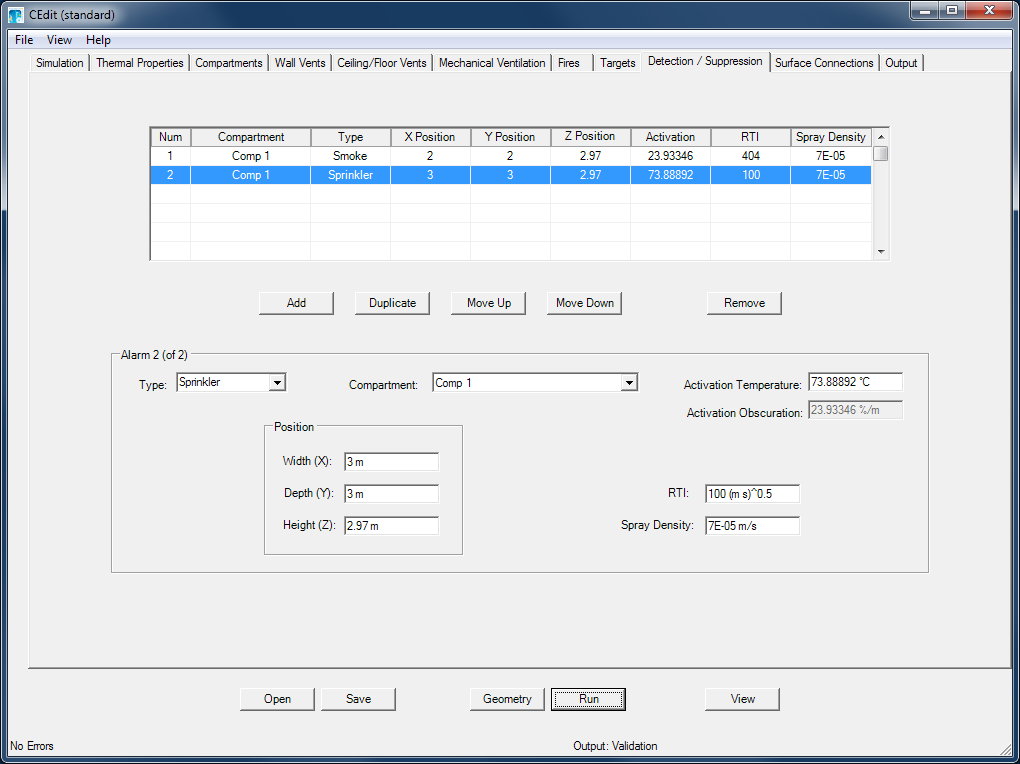
\includegraphics[width=6.5in]{FIGURES/Detector_Tab}
\caption[The CFAST Detection/Suppression Tab]{The CFAST Detection/Suppression Tab.}
\end{center}
\end{figure}

\begin{description}
\item[ID]  The selected name must be unique (i.e., not the same as another sprinkler or detector in the same simulation).

\item[Type] type of detector, select smoke detector, heat detector, or sprinkler.

\item[Compartment] the compartment in which the detector or sprinkler is located.

\item[Activation Temperature] (default units: \degc, default value: dependent on type): the temperature at or above which the detector link activates.

\item[Activation Obscuration] (default units: \%/m, default value: 23.93 \%/m (8 \%/ft)): the obscuration at or above which the detector link activates.

\item[Width (X)] Position (default units: m, default value: none): position of the object as a distance from the left wall of the compartment (X direction).

\item[Depth (Y)] Position (default units: m, default value: none): position of the detector or sprinkler as a distance from the front wall of the compartment (Y direction).

\item[Height (Z)] Position (default units: m, default value: none): position of the object as a distance from the floor of the compartment (Z direction).

\item[RTI] (default units: (m$\cdot$s)$^{1/2}$, default value: none): the Response Time Index (RTI) for the sprinkler or detection device.

\item[Spray Density] (default units: m/s, default value: none): the amount of water dispersed by a sprinkler.  The units for spray density are length/time, derived by dividing the volumetric flow rate by the spray area. The suppression calculation is based upon an experimental correlation by Evans~\cite{Evans:1993}.
\end{description}

\graybox{
Care should be taken when specifying detectors to activate based on smoke obscuration since the only calculation included in CFAST is a simple two-zone calculation of soot concentration that does not include the impact of an initial ceiling layer as is done for temperature-based calculations. Often, the activation of smoke alarms is simulated with a temperature-based criterion (in CFAST as a heat alarm), typically in the range of 5~\degc to 10~\degc above ambient. Davis and Notarianni  studied the activation of heat and smoke alarms in small and large compartments \cite{Davis:1996}. They conclude that a temperature rise of approximately 5~\degc corresponded to activation of ionization alarms for a range of fire sources and ceiling heights. The Nuclear Regulatory Commission includes a default value of 10~\degc with an RTI value of 5 (m$\cdot$s)$^{1/2}$ in NUREG-1805 \cite{NRCNUREG1805}. \\

Several cautions should be observed when using estimates of sprinkler suppression within the model: 1)~The first sprinkler activated controls the effect of the sprinkler on the heat release rate of the fire.  Subsequent sprinklers which may activate have no additional effect on the fire simulation. 2)~The fire suppression algorithm assumes the effect of the sprinkler is solely to reduce the heat release rate of the fire. Any effects of the sprinkler spray on gas temperatures or mixing within the compartment are ignored. 3)~The sprinkler always reduces the heat release rate of the fire. The ability of a fire to overwhelm an under-designed sprinkler is not modeled. 4) Since the dynamics of the sprinkler and direct effects of the spray on gas temperatures and velocities are not modeled, calculated times of activation of secondary sprinklers and / or detectors after the first sprinkler is activated should not be modeled since the impact of the first sprinkler on the activation of additional sprinklers is not included in the CFAST model.}




\chapter{Surface Connections}
\label{info:CONN}
\begin{figure}[h!]
\begin{center}
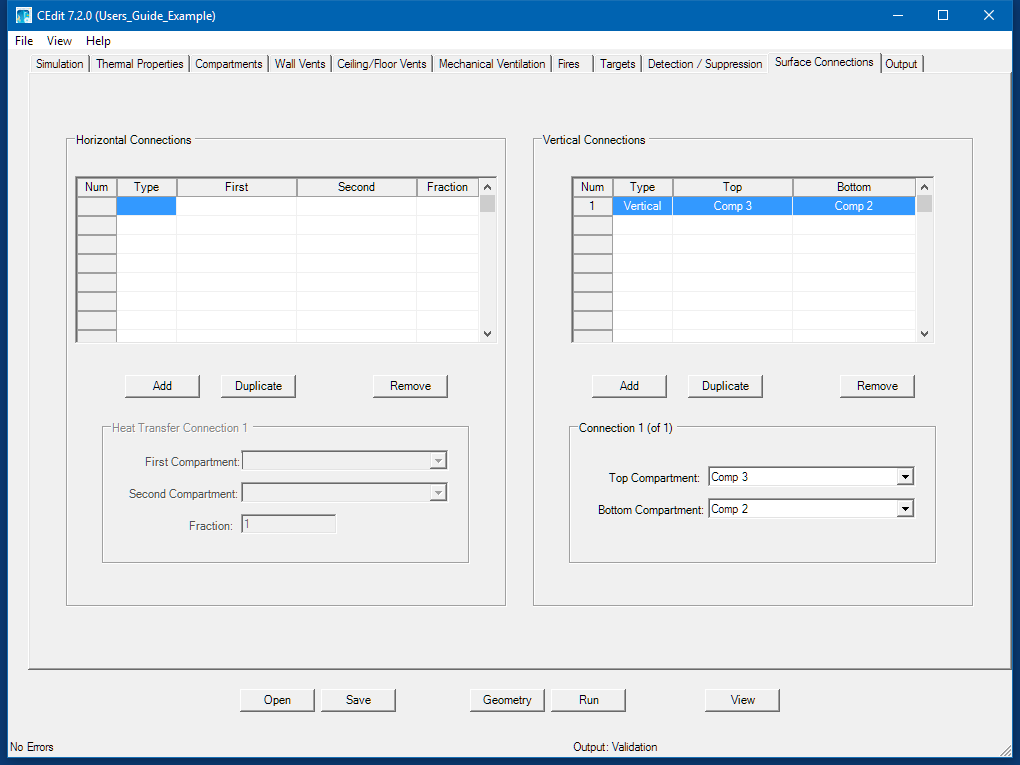
\includegraphics[width=6.5in]{FIGURES/Surface_Connection_Tab}
\caption[The CFAST Surface Connections Tab]{The CFAST Surface Connections Tab.}
\end{center}
\end{figure}

The Surface Connections page allows the user to define heat transfer between compartments in a simulation. Energy can be transferred from compartment to compartment through solid boundaries (walls, ceilings and floors) by means of conduction. The heat transfer between connected compartments is modeled by setting the boundary condition for the outside surface of a compartment to the temperature of the outside surface of the  connected compartment.   As before, temperatures are determined by the solver so that the heat flux striking the wall surface (both interior and exterior) is consistent with the temperature gradient at that surface.

\begin{description}
\item[First Compartment] First of the compartments whose walls are connected for horizontal heat transfer.

\item[Second Compartment] Second of the compartments whose walls are connected for horizontal heat transfer.

\item[Fraction] Specifies the fraction of the vertical surface areas of the compartments which are connected. The fraction specifies the fraction of the vertical surface area of the first compartment that connects the first and second compartment pair.

\item[Top Compartment] The top or first of the two compartments to be connected by a vertical heat transfer connection. The connection is through the floor of this compartment.

\item[Bottom Compartment] The bottom or second of the two compartments to be connected by a vertical heat transfer connection. The connection is through the ceiling of this compartment.
\end{description}

\graybox{Consider two compartments that share a single wall. Both compartments are 1 m x 1 m x 1 m in size. The resulting horizontal heat transfer connections would be 0.25 for both compartments since they share 1 m$^2$ of a total wall surface of 4 m$^2$. If the compartments are of different size, then the fraction would be different for the two directions. For example, if compartment 1 is 1 m x 1 m x 1 m and compartment 2 is 2 m x 2 m x 2 m, then the connection from 1$>$2 is 0.25 and the connection from 2$>$1 is 0.125.

For horizontal heat transfer, you must include a connection for each compartment. For example, for a connection between compartment 1 and compartment 2, you must include a connection from 1 to 2 AND a connection from 2 to 1.  For consistency, the fraction for each compartment needs to specify equal areas in the two compartments.  Fractions for connections should add to unity.  An error is generated if the fractions for a compartment add to greater than unity. If the fractions for a compartment add to less than unity, the remaining surface area will be assigned to be connected to the outdoors.}




\chapter{Visualization}

Calculated results from a CFAST simulation can be visualized using Smokeview \cite{Smokeview_Users_Guide_6}. This allows the user to see the compartment geometry and connections or view the results of the simulation visually. In addition to a simplified view of the layer temperatures and vent flows, more detailed estimates of gas temperature, gas velocity, vent flow velocity, target temperature, and detector status can be visualized.

\begin{figure}[h!]
\begin{center}
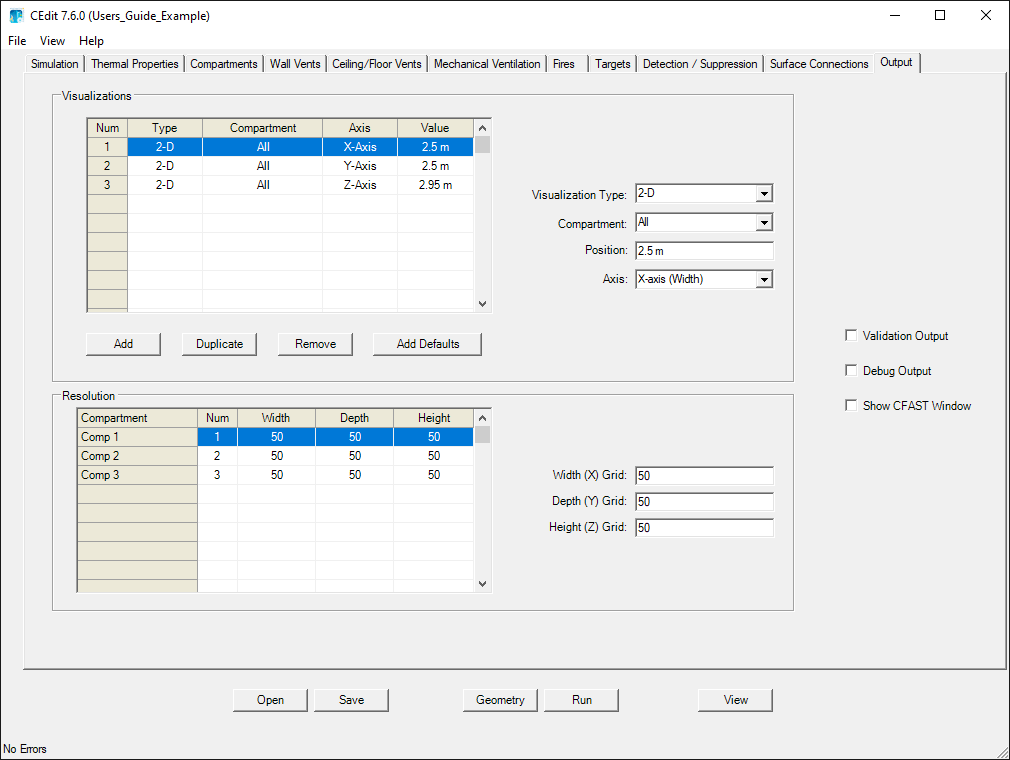
\includegraphics[width=6.5in]{FIGURES/Visualizations_Tab}
\caption[The CFAST Visualizations Tab]{The CFAST Visualizations Tab.}
\end{center}
\end{figure}

\section{Adding Visualizations}
\label{info:ISOF}
\label{info:SLCF}

\begin{description}
\item[Visualization Type] ( default value: 2-D): The type of visualization to be included. Choose from 2-D (a single plane slice of temperature at the position and axis specified), 3-D (a set of three animated slices whose position can be moved along its respective axis, or Isosurface (a fixed 3-D surface where the gas temperature is equal to the value specified. See the Smokeview documentation \cite{Smokeview_Users_Guide_6} for details on the use of Smokeview.

\item[Compartment] (default value: All): Visualizations can be placed in a single compartment or at the same position and axis in all compartments.

\item[Value] (default units: m, default value: 0 m): Position along the specified axes where the slice is placed measured from the compartment origin for the selected axis (0,0,0 is the bottom left corner of the compartment. See page \pageref{Compartment_Geometry}).

\item[Axis] (default value: X-axis (Width)): Axis perpendicular to the specified slice.  The slice is place perpendicular to the selected axis (the Y-Z plane for the X-Axis; the X-Z plane for the Y-Axis, and the X-Y plane for the Z-Axis)

\item[Temperature] (default units \degc, default value: none): Specified gas temperature for the selected isosurface.
\end{description}

%Not sure what is trying to be said here but I think it is a fail.
\graybox{
Use the Add Defaults button to add a default set of visualizations for the current simulation. A slice file entry is created at the center of each compartment in the x (width) and y (depth) directions along with one near the ceiling in the z direction. A 3-D slice file entry is created for each compartment as well.
}

\section{Visualization Resolution}
\label{info:SLCF2}

By default, slice files are generated with a grid of 50 data points in each direction for each compartment specified. If desired, the grid spacing can be adjusted up or down individually by compartment. Specifying a larger number of data points can \textit{dramatically} slow program execution since the gas temperature and velocity are evaluated at each grid location every time a Smokeview output is specified.  The default value should be appropriate for most simulations.

\begin{description}
\item[Width (X) Grid] (default unites: n/a, default value: 50): slices included along the X axis for each compartment are uniformly divided into the specified number of data points.

\item[Width (Y) Grid] (default unites: n/a, default value: 50): slices included along the Y axis for each compartment are uniformly divided into the specified number of data points.

\item[Width (Z) Grid] (default unites: n/a, default value: 50): slices included along the Z axis for each compartment are divided into the specified number of data points.
\end{description}

Sample visualizations are included below.

\begin{figure}[h!]
\begin{center}
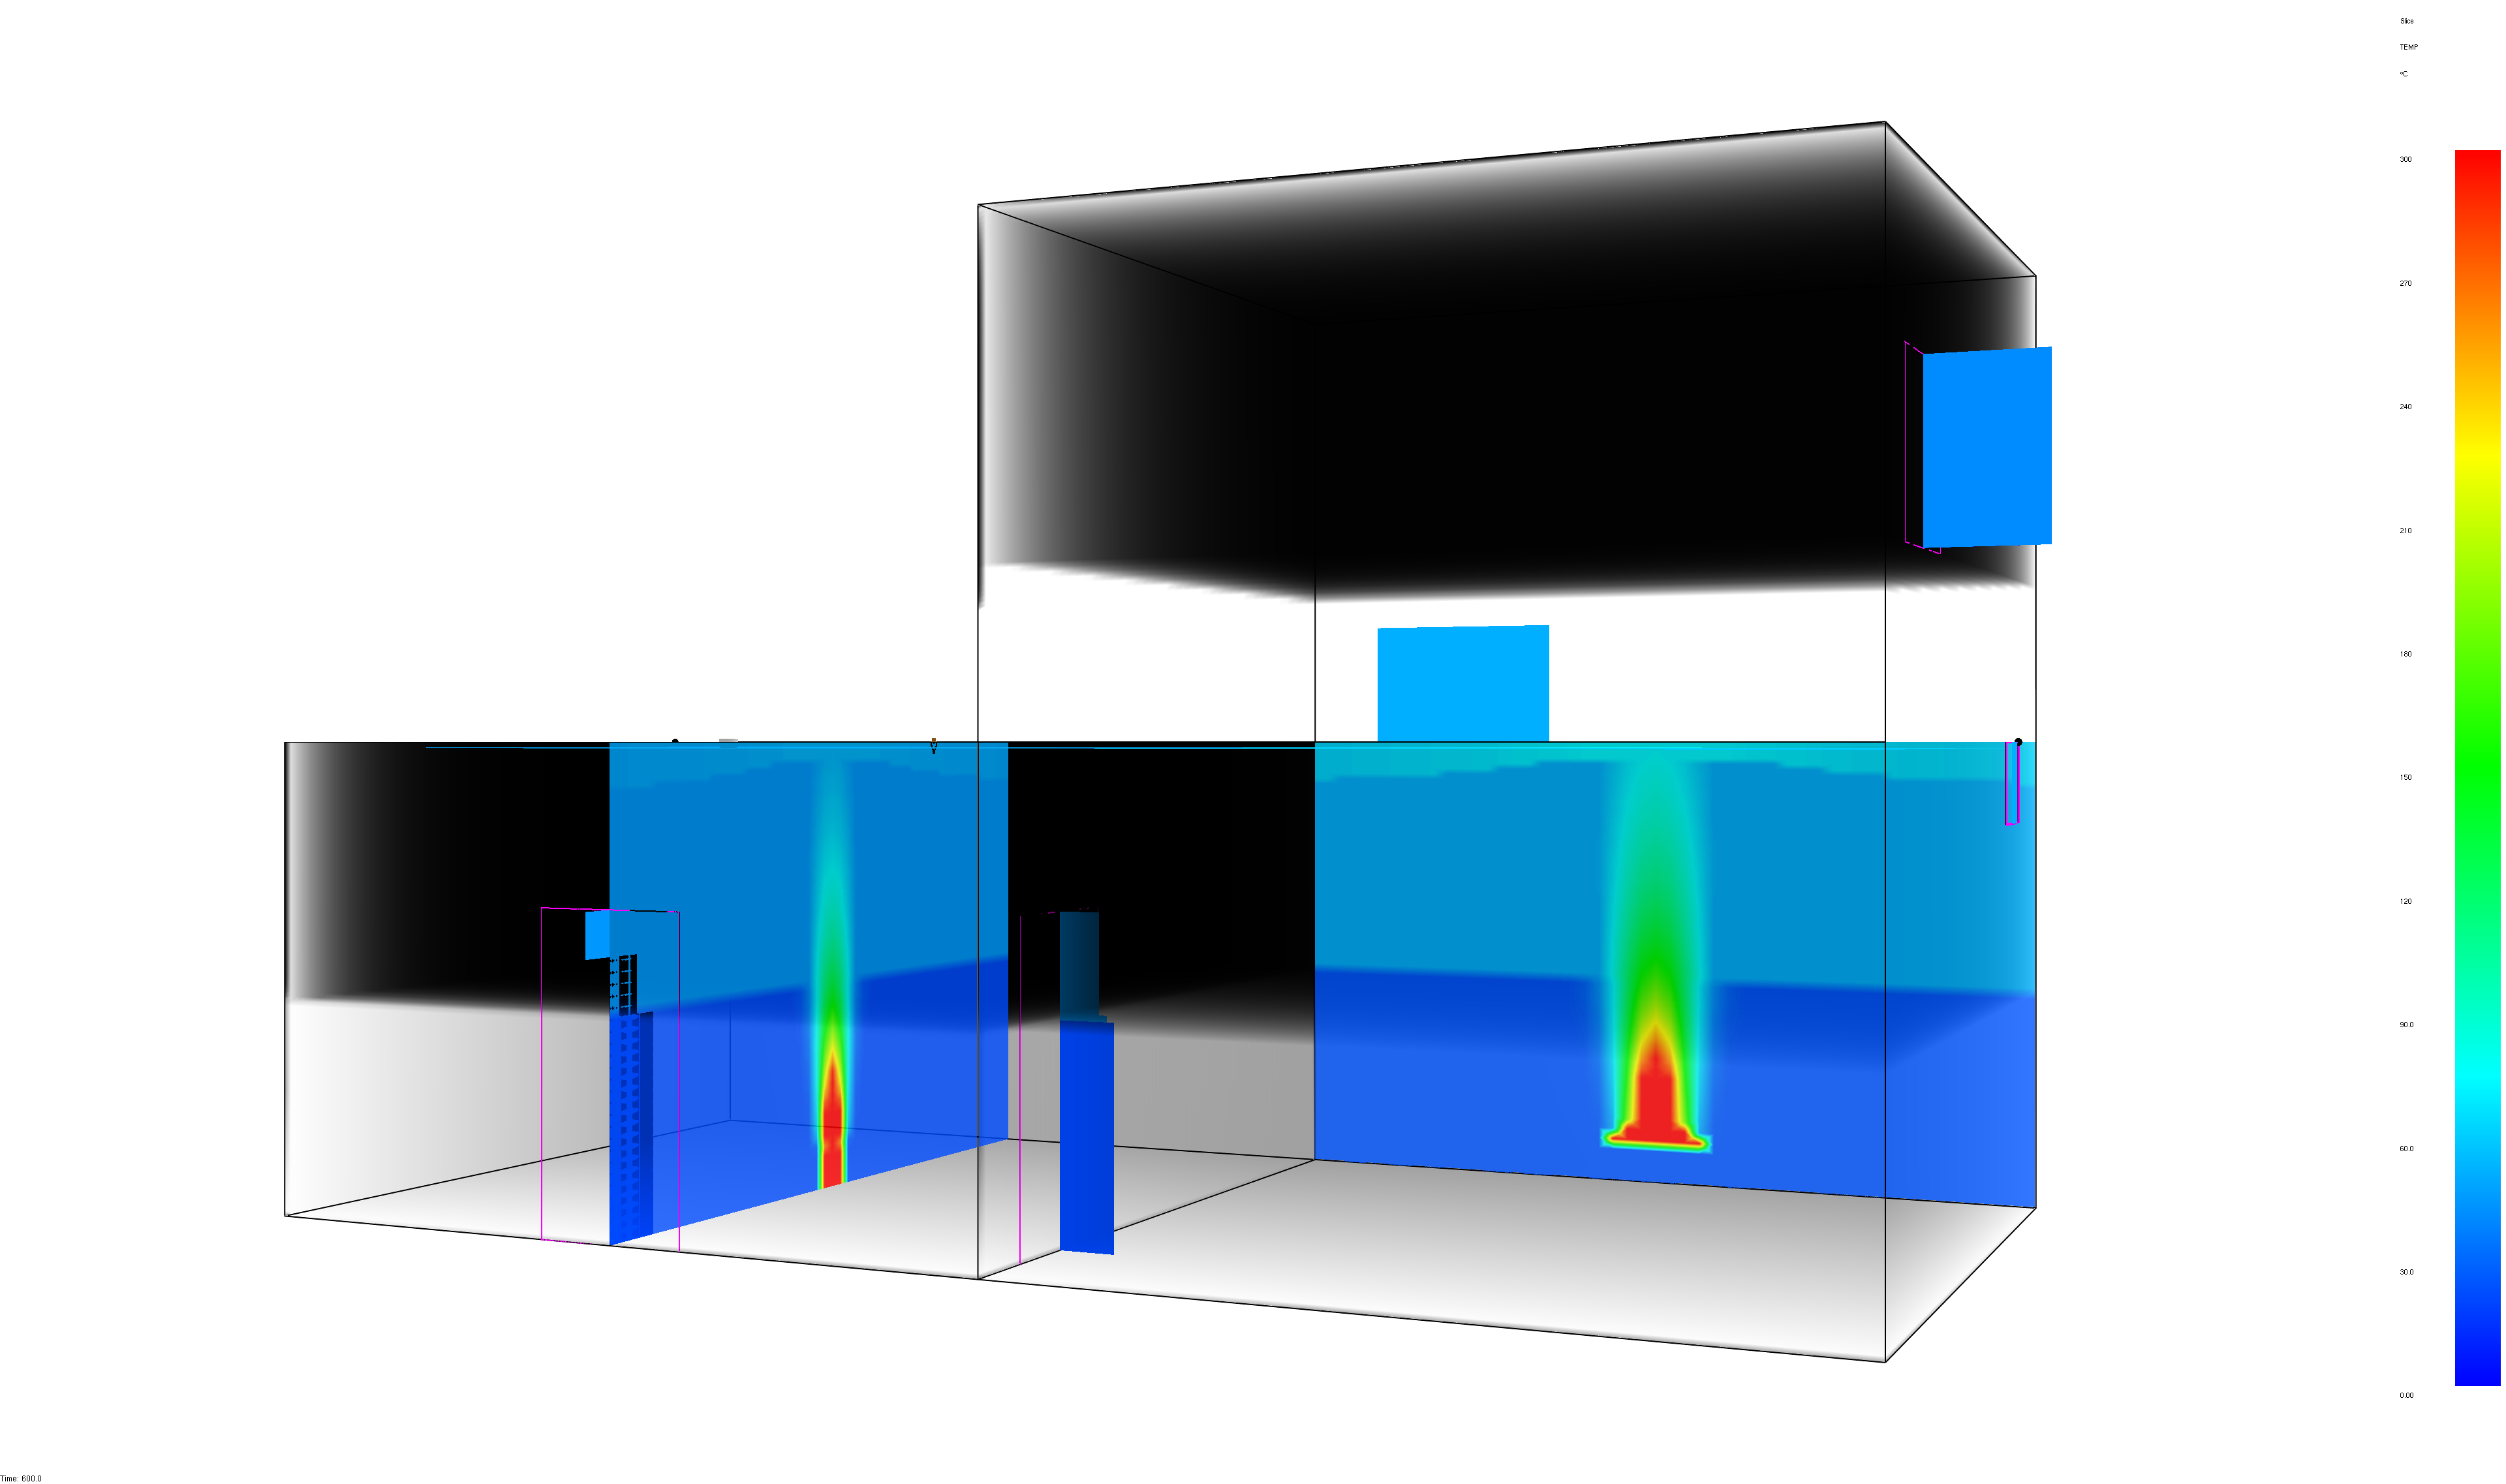
\includegraphics[width=6.5in]{FIGURES/SMV_Sample}
\caption{example Smokeview Visualization for a Three Compartment Test Case with Two Fires (\ct User\_Guide\_Example.in)}
\end{center}
\end{figure}

\begin{figure}[h!]
\begin{center}
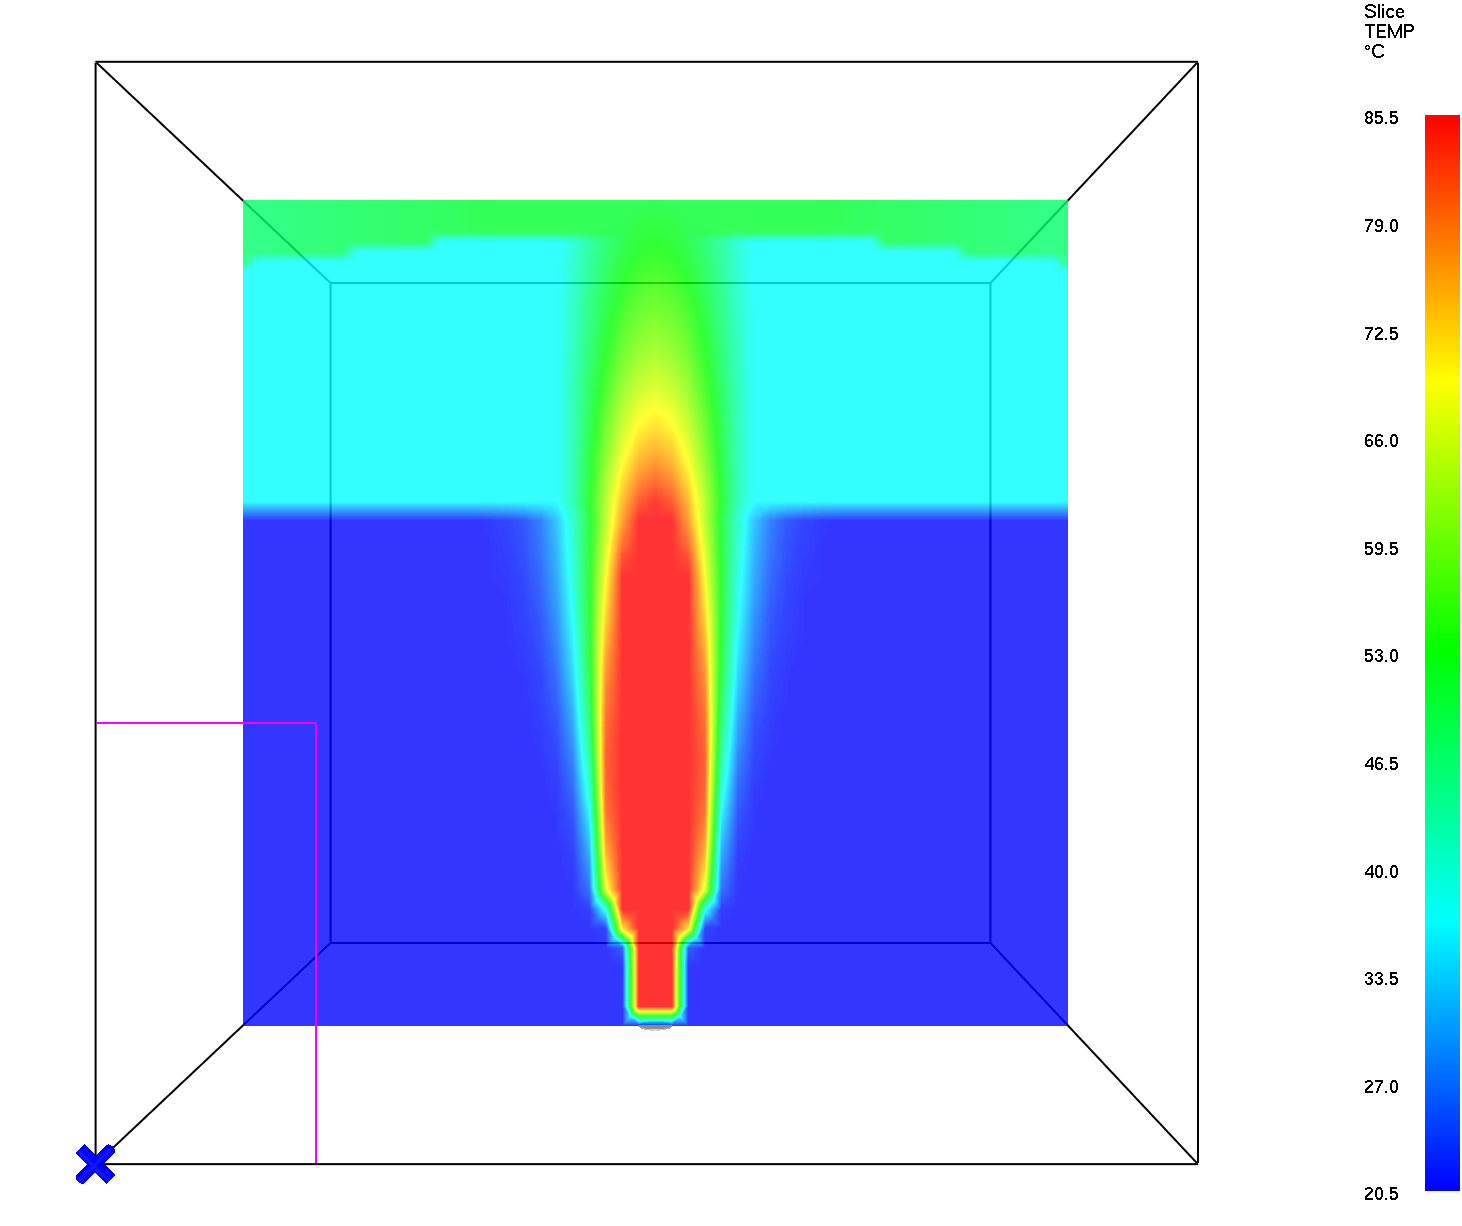
\includegraphics[width=6.5in]{FIGURES/SMV_Temperature}
\caption{Smokeview Visualization of Gas Temperature with a Single Fire}
\end{center}
\end{figure}

\begin{figure}[h!]
\begin{center}
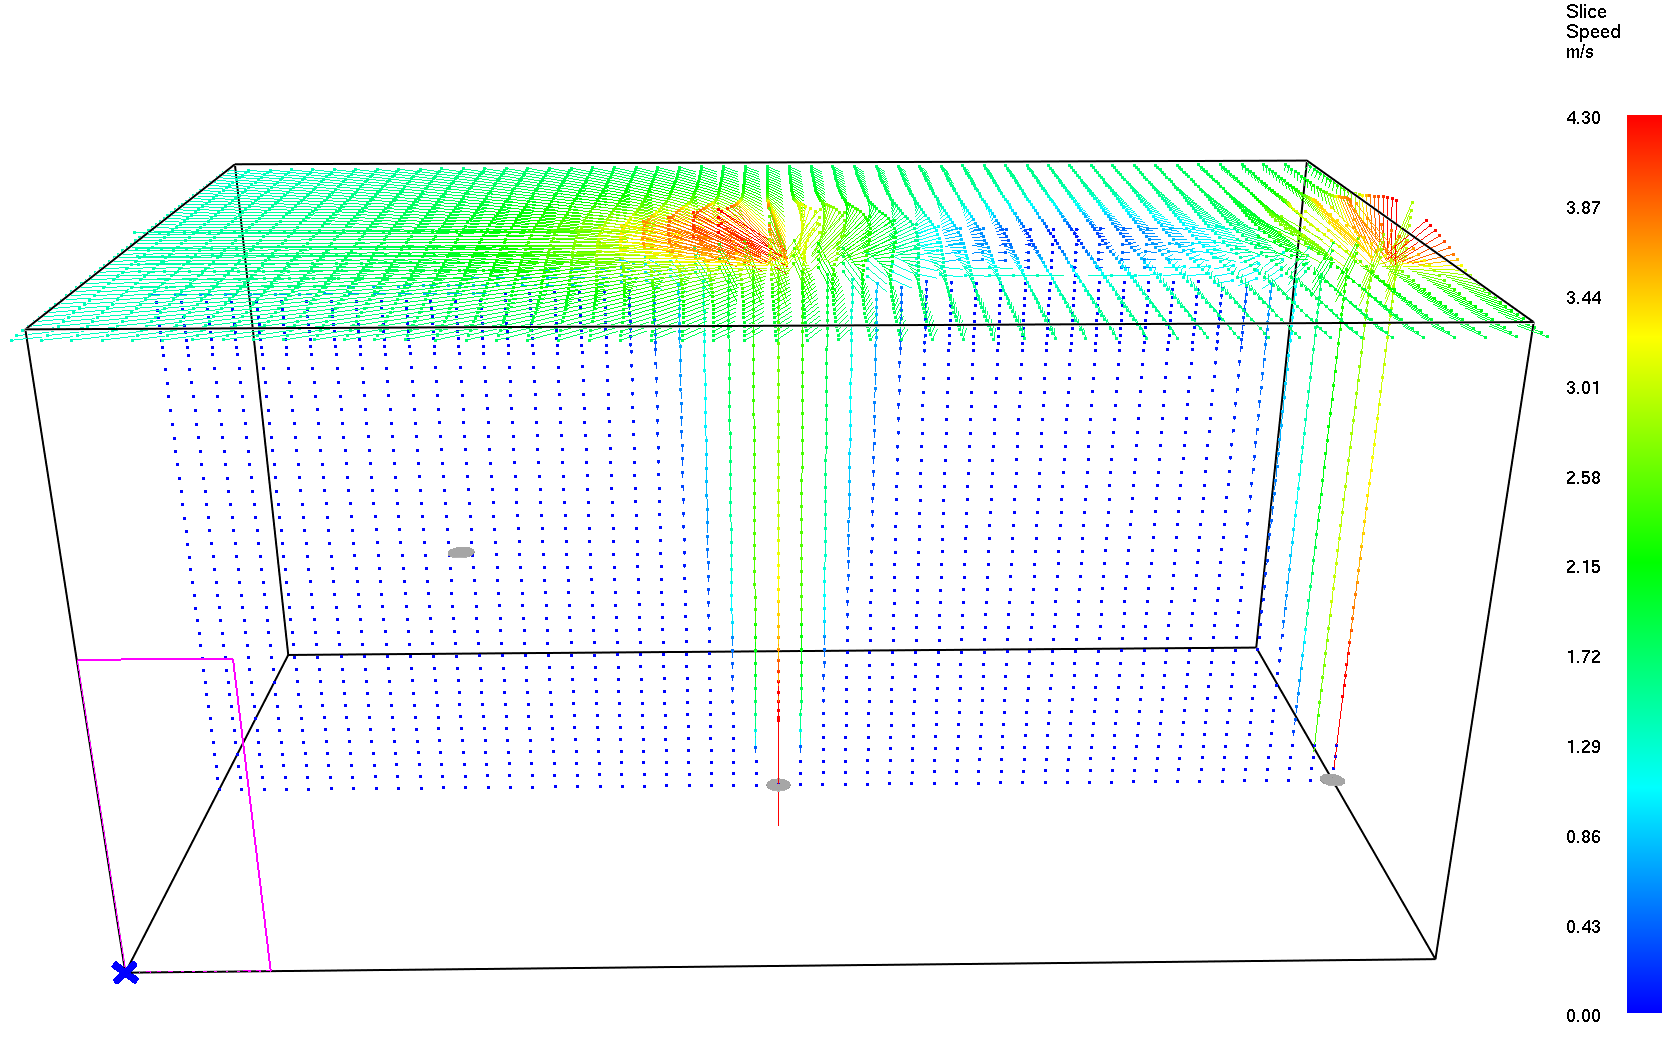
\includegraphics[width=6.5in]{FIGURES/SMV_Velocity}
\caption{Smokeview Visualization of Gas Velocity with Two Fires}
\end{center}
\end{figure}

\begin{figure}[h!]
\begin{center}
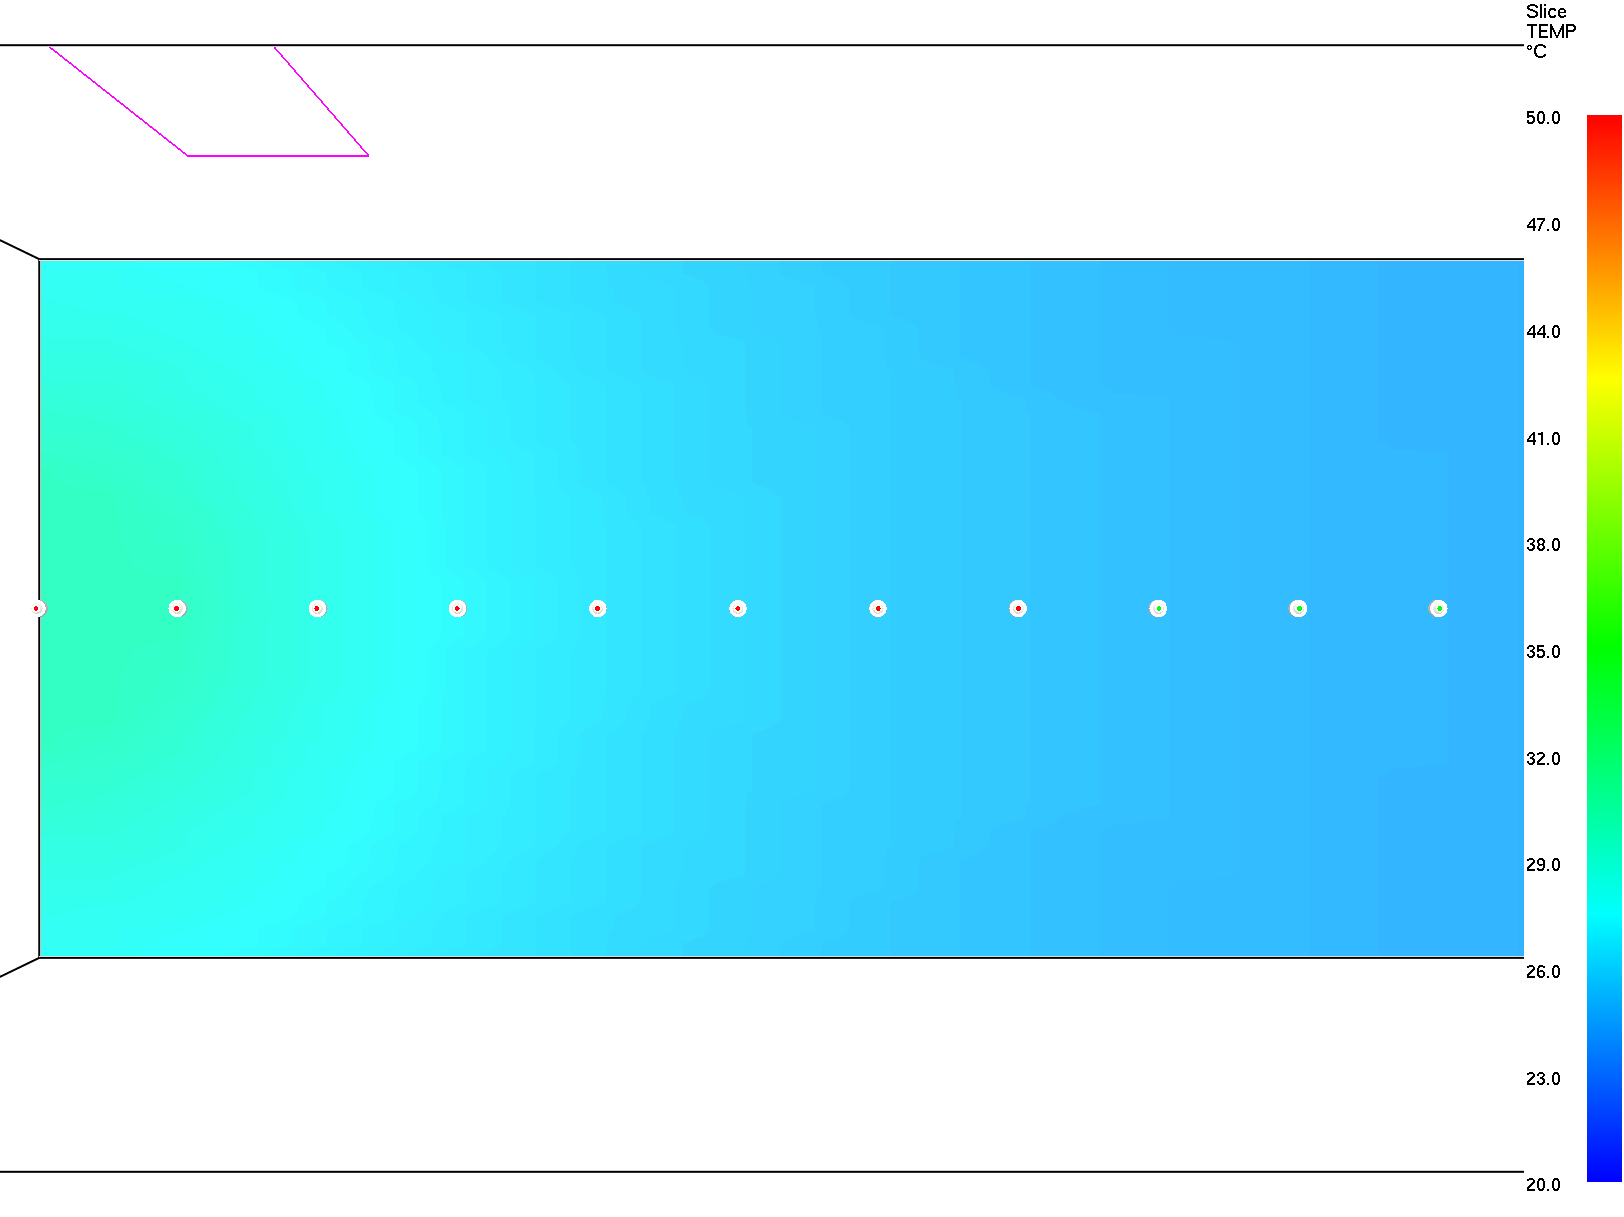
\includegraphics[width=6.5in]{FIGURES/SMV_Detectors}
\caption{Smokeview Visualization of Detector Activation in a Corridor}
\end{center}
\end{figure}

\section{Output Options}

By default, CFAST generates a set of output files that includes a formatted readable output and a set of spreadsheet files.  Options are available to modify the output files.  The default output should be appropriate for most simulations.

\begin{description}
    \item[CFAST Validation Output] If checked, this item directs the CFAST model to output abbreviated headings for spreadsheet columns that are better for automated processing of the data.
    \item[Debug Output] If checked, CFAST will create a detailed output spreadsheet that contains values of all the solution variables at each successful solution time step. This file is typically only of use to model developers diagnosing a problem with the model.
    \item[Show CFAST Window] If checked, this item allows the user to see the windows command prompt that is used to execute the CFAST model when the Model Simulation, CFAST menu item is used.  By default, this is not checked.  Normally, this can be left unchecked.  For troubleshooting, this can be selected to see additional details of the calculation as it progresses.
\end{description}





\chapter{Output from CFAST}
\label{Output_Chapter}

The output of CFAST includes the temperatures of the upper and lower gas layers within each compartment, the ceiling/wall/floor temperatures within each compartment, the visible smoke and gas species concentrations within each layer, target temperatures and sprinkler activation time.  The amount of information can be very large, especially for complex geometries and long simulations.

\section{Compact Output}

The default output to the console is called the compact form, and shows the basic information about a scenario, including layer temperatures and the size of fires. Default text output provides a simple overview for the user to make sure the case runs as expected.
\begin{lstlisting}[basicstyle=\scriptsize]
 Time =   1800.0 seconds.

 Compartment   Upper   Lower   Inter.  Pyrol     Fire      Pressure  Ambient
               Temp.   Temp.   Height  Rate      Size                Target
               (C)     (C)     (m)     (kg/s)    (W)       (Pa)      (W/m^2)
 -----------------------------------------------------------------------------
    1          113.4    33.3    1.4     1.393E-02 3.000E+05-0.790      523.
  Outside                                         0.00
\end{lstlisting}
The first column contains the compartment number.  On each row with its compartment number from left to right is the upper layer temperature, lower layer temperature, the height of the interface between the two layers, the total pyrolysis rate, and finally the total fire size.  The only value given for the outside is the total heat release rate of fires venting to the outside.

\section{Detailed Outputs}

The following sections describe each of the outputs from the model.  Each section refers to a specific part of the print out and appears in the order the output appears. A description of each option follows.

\subsection{Output for Initialization}

This option prints the initial conditions to the output before the actual run starts.  This merely mimics the inputs specified by the user in the input data file  The initial conditions break down into seven sections.  Each is described below with the section name. The following explanation uses the output from the case STANDARD.IN. STANDARD.IN is included in the distribution. Please note, there are no mechanical ventilation, horizontal vents or detectors in this example, so the section discussing these phenomena are from additional data files.

\subsubsection{Overview}

The overview gives a general description of the case.  The output is fairly self explanatory. ``Doors, ...'' is the total number of horizontal natural flow vent connections in all compartments of the simulation.  ``Ceil. Vents, ...'' gives the total number of vertical natural flow vent connections in all compartments of the simulation.  The last header on the line ``MV Connections'' has the total number mechanical flow connections to all compartments in the simulation. Times in these outputs come from the TIMES input. All times are in s.
\begin{lstlisting}[basicstyle=\tiny]
CFAST

Version          : CFAST 7.2.0
Revision         : Gitv7.0.1-132-gf03a791
Revision Date    : Tue Feb 2 12:54:53 2016 -0500
Compilation Date : Tue 02/02/2016  12:55 PM

Data file: C:\Users\rpeacoc\Documents\Visual Studio 2013\Projects\cfast\Bin\Data\standard.in
Title: Users Guide Example Case


OVERVIEW


Compartments    Doors, ...    Ceil. Vents, ...    MV Connects
-------------------------------------------------------------
   3               3             1                    2

Simulation     Output         Smokeview      Spreadsheet
Time           Interval       Interval       Interval
   (s)            (s)            (s)            (s)
--------------------------------------------------------
  3600          50             10             10
\end{lstlisting}

\subsubsection{Ambient Conditions}

This section, like the overview section, needs little elaboration.  It gives the starting atmospheric conditions for the simulation both for outside and inside the structure. Data for these outputs come from the TAMB and EAMB inputs. Temperatures are in K, pressure in Pa, elevations in m, and wind speed in m/s. Wind Power is the dimensionless power law coefficient from the WIND input.
\begin{lstlisting}[basicstyle=\tiny]
AMBIENT CONDITIONS

Interior       Interior       Exterior       Exterior
Temperature    Pressure       Temperature    Pressure
  (C)            (Pa)           (C)            (Pa)
-----------------------------------------------------
    20.          101325.          20.          101325.
\end{lstlisting}

\subsubsection{Compartments}

The compartments section gives a summary of the geometry for the simulation.  A simple table summarizes the geometry with compartments running down the page in numerical order.  The various dimensions for each compartment are on the row with its compartment number.  Two columns need explanation.  The second to last column ``Ceiling Height'' gives the height of the ceiling relative to the station height in the Ambient Conditions section.  Similarly the ``Floor Height'' refers to the height of the floor above the station height.

\begin{lstlisting}[basicstyle=\tiny]
COMPARTMENTS

Compartment  Name                Width        Depth        Height       Floor        Ceiling
                                                                        Height       Height
                                 (m)          (m)          (m)          (m)          (m)
------------------------------------------------------------------------------------------------
    1               Comp 1        5.00         5.00         3.00         0.00         3.00
    2               Comp 2        5.00         5.00         3.00         0.00         3.00
    3               Comp 3        5.00         5.00         3.00         3.00         6.00
\end{lstlisting}


\subsubsection{Horizontal Natural Ventilation}

This is the first table in the vent connections section.  Each row in the table characterizes one vent.  The first two columns contain the two compartments connected by the vent.  Each vent is ordered first by the lower number of the two compartments and then the numeric order of the second compartment.  The third column gives the vent number.  Column four is the width of the vent.  The next two columns report the sill and soffit height for the vent relative to the floor of the first compartment.  The seventh and eighth columns have a second listing of the sill and soffit height, this time relative to the station height.

\begin{lstlisting}[basicstyle=\tiny]
VENT CONNECTIONS

Horizontal Natural Flow Connections (Doors, Windows, ...)

From         To           Vent    Width  Sill    Soffit  Open/Close  Trigger           Initial  Initial   Final  Final
Compartment  Compartment  Number         Height  Height  Type        Value     Target  Time     Fraction  Time   Fraction
                                  (m)    (m)     (m)     (m)         (C/W/m^2)         (s)                (s)
-------------------------------------------------------------------------------------------------------------------------
Comp 1       Outside      1       1.00   0.00    2.00    Time                          0.00     1.00      0.00   1.00
Comp 1       Comp 2       1       1.00   0.00    2.00    Time                          0.00     1.00      0.00   1.00
Comp 3       Outside      1       1.00   1.00    2.00    Time                          0.00     1.00      0.00   1.00
\end{lstlisting}
From compartment, to compartment, vent number, width, sill height, and soffit height all come directly from the HVENT specifications in the input data file. Vent opening and closing information can be specified by time, by an associated time / fraction history by a RAMP input or by an associated target to trigger a change in the vent opening by temperature or heat flux.

\subsubsection{Vertical Natural Ventilation}

The first column is the upper compartment.  The upper compartment is the compartment where the vent opens into the floor.  The second column is the lower compartment where the vent is in the ceiling. Each vent connection between compartment pairs is also identified by a vent number index beginning with 1. The fourth column describes the shape of the vent, which can be either round or square.  The fifth column gives the area of the vent. Vent opening and closing information can be specified by time, by an associated time / fraction history by a RAMP input or by an associated target to trigger a change in the vent opening by temperature or heat flux.
\begin{lstlisting}[basicstyle=\tiny]
Vertical Natural Flow Connections (Ceiling, ...)

Top           Bottom        Vent    Shape    Area     Open/Close  Trigger               Initial    Initial     Final    Final
Compartment   Compartment   Number                    Type        Value      Target     Time       Fraction    Time     Fraction
                                             (m^2)                (C/W/m^2)             (s)                    (s)
--------------------------------------------------------------------------------------------------------------------------------
Comp 3        Comp 2         1      Round    1.00     RAMP # 1  
\end{lstlisting}
Top compartment, bottom compartment, shape, and area come from the VVENT specifications in the input data file. Relative height is the height of the vent above the floor of the bottom compartment and absolute height is the height of the vent above the station elevation.

\subsubsection{Mechanical Flow Connections}

This section lists all connections to compartments and fans that connect between compartments. The table lists, in order, the compartments connected by the fan, a numeric index assigned to the fan beginning with 1.  A fan actually draws air from the first or ``from'' compartment and pushes it to the second or ``to'' compartment. The fourth column is the cross-sectional area of the duct connection to the chosen compartment. Vent opening and closing information can be specified by time, by an associated time / fraction history by a RAMP input or by an associated target to trigger a change in the vent opening by temperature or heat flux.

\begin{lstlisting}[basicstyle=\tiny]
FANS

From          To            Fan      Area    Flowrate   Open/Close  Trigger             Initial   Initial    Final   Final
Compartment   Compartment   Number                      Type        Value     Target    Time      Fraction   Time    Fraction
                                     (m^2)   (m^3/s)                (C/W/m^2)           (s)                  (s)
-----------------------------------------------------------------------------------------------------------------------------
Outside       Comp 1        1        0.00    0.02       Time                            0.00      1.00       0.00    1.00
Comp 2        Outside       2        0.00    0.02       Time                            0.00      1.00       0.00    1.00
\end{lstlisting}

\subsubsection{Ventilation Opening Ramp Specifications}

Opening and closing of vents in CFAST can be specified by a series of times and opening fractions for a specified vent. By default, all vents are open at the beginning of a simulation and remain open throughout the simulation.  With the RAMP input, the opening of a vent can change of time. 

\begin{lstlisting}[basicstyle=\tiny]
VENT RAMPS

Type  From         To            Vent
      Compartment  Compartment   Number
                                                    (s)    (s)    (s)    (s)    (s)    (s)    (s)    (s)    (s)    (s)
----------------------------------------------------------------------------------------------------------------------
V     Comp 3       Comp 2        1       Time         0    100    500
                                         Fraction  0.00   0.50   1.00
\end{lstlisting}

\subsubsection{Thermal Properties}

The thermal properties section is broken into two parts.  The first part is a table that lists the material for each surface of each compartment.  The compartments appear as rows down the page in numerical order.  From left to right next to the compartment number comes the material for the ceiling, wall and floor.  The second part lists the properties of each material used in the simulation. For each listing of a material, the name is followed by the conductivity, specific heat, density, thickness and emissivity. In addition to materials for compartment surfaces, any thermal properties specified for targets are also listed (this may include thermal properties for gaseous materials specified as fire sources in a simulation.

\begin{lstlisting}[basicstyle=\tiny]
THERMAL PROPERTIES

Compartment    Ceiling      Wall         Floor
-----------------------------------------------
Comp 1       CONCRETE     CONCRETE     CONCRETE
Comp 2       CONCRETE     CONCRETE     CONCRETE
Comp 3       CONCRETE     CONCRETE     CONCRETE


Name    Conductivity      Specific Heat     Density        Thickness     Emissivity
-----------------------------------------------------------------------------------
CONCRETE     1.75           1.000E+03       2.200E+03       0.150           0.940
DEFAULT     0.120            900.            800.           1.200E-02       0.900
\end{lstlisting}
Material choices of the ceiling, walls, and floors come from the CEILI, WALLS, and FLOOR specifications in the input data file. Units for thermal properties are standard S.I. units.  For thermal conductivity, W/m K; for specific heat, J/kg K; for density, kg/m$^3$; for thickness, m; emissivity is dimensionless.


\subsubsection{Fires}

The fire section lists all the information about the main fire and any object fires that might exist.  All the information for each fire is listed separately.  If there is a main fire, it comes first.  Each fire listing has the same form.  First is the name of the fire followed by a list of general information.  Listed left to right is the compartment the fire is in, the type of fire, the initial x (width), y (depth), z (height) position of the fire, the relative humidity, the lower oxygen limit, and finally the radiative fraction for the fire.

A table of time history curves for the fire follows.  The table contains all the time history curves for the fire.  Each row on the table is a specific time given in the left most column.  The rest of the columns give the values at that particular time.  The column headers indicate each input quantity and correspond to specific keywords in the fire definition. The headings are defined as follows: `Mdot' is pyrolysis rate; `Hcomb' is the heat of combustion; `Qdot' is the heat release rate; `Zoffset' is height of the fire above the base z-position; `Soot' is the fraction of the fuel mass converted to soot during combustion; `CO' is the fraction of the fuel mass converted to carbon monoxide during combustion; `HCN' is the fraction of the fuel mass converted to hydrogen cyanide during combustion; `HCl' is the fraction of the fuel mass converted to hydrogen chloride during combustion; `CT' is the concentration-time product; and `TS' is the fraction of fuel mass converted to trace species during combustion.

\begin{lstlisting}[basicstyle=\tiny]
FIRES


Name: bunsen   Referenced as object #  1 Normal fire

Compartment    Fire Type       Position (x,y,z)     Relative    Lower O2    Radiative
                                                    Humidity    Limit       Fraction
-------------------------------------------------------------------------------------
Comp 1         Constrained     2.50   2.50   0.00   50.0        15.00        0.33


Chemical formula of the fuel
Carbon     Hydrogen  Oxygen    Nitrogen  Chlorine
--------------------------------------------------
  1.000     4.000     0.000     0.000     0.000


  Time      Mdot      Hcomb     Qdot      Zoffset   Soot      CO        HCN       HCl       TS
  (s)       (kg/s)    (J/kg)    (W)       (m)       (kg/kg)   (kg/kg)   (kg/kg)   (kg/kg)   (kg/kg)
------------------------------------------------------------------------------------------------------
     0.      0.0      5.00E+07   0.0       0.0       0.0      1.05E-03   0.0       0.0       0.0
    60.     2.00E-03  5.00E+07  1.00E+05   0.0       0.0      1.05E-03   0.0       0.0       0.0
   120.     3.00E-03  5.00E+07  1.50E+05   0.0       0.0      1.05E-03   0.0       0.0       0.0
   180.     4.00E-03  5.00E+07  2.00E+05   0.0       0.0      1.05E-03   0.0       0.0       0.0
   240.     3.00E-03  5.00E+07  1.50E+05   0.0       0.0      1.05E-03   0.0       0.0       0.0
   300.     2.50E-03  5.00E+07  1.25E+05   0.0       0.0      1.05E-03   0.0       0.0       0.0
   360.     2.00E-03  5.00E+07  1.00E+05   0.0       0.0      1.05E-03   0.0       0.0       0.0
   420.     1.80E-03  5.00E+07  9.00E+04   0.0       0.0      1.05E-03   0.0       0.0       0.0
   480.     1.60E-03  5.00E+07  8.00E+04   0.0       0.0      1.05E-03   0.0       0.0       0.0
   540.     1.50E-03  5.00E+07  7.50E+04   0.0       0.0      1.05E-03   0.0       0.0       0.0
  1800.     1.50E-03  5.00E+07  7.50E+04   0.0       0.0      1.05E-03   0.0       0.0       0.0


Name: Wood_Wall   Referenced as object #  2 Wall   fire

Compartment    Fire Type       Position (x,y,z)     Relative    Lower O2    Radiative
                                                    Humidity    Limit       Fraction
-------------------------------------------------------------------------------------
Comp 2         Constrained     2.50   5.00   0.00   50.0        15.00        0.33


Chemical formula of the fuel
Carbon     Hydrogen  Oxygen    Nitrogen  Chlorine
--------------------------------------------------
  6.000    10.000     5.000     0.000     0.000


  Time      Mdot      Hcomb     Qdot      Zoffset   Soot      CO        HCN       HCl       TS
  (s)       (kg/s)    (J/kg)    (W)       (m)       (kg/kg)   (kg/kg)   (kg/kg)   (kg/kg)   (kg/kg)
------------------------------------------------------------------------------------------------------
     0.      0.0      1.81E+07   0.0       0.0      2.00E-02  2.00E-02   0.0       0.0       0.0
  8000.     5.52E-02  1.81E+07  1.00E+06   3.0      2.00E-02  2.00E-02   0.0       0.0       0.0
\end{lstlisting}
All of the inputs for the main fire come from the fire specifications in the input data file. Data for the object fire comes from the object data file included with the CFAST software. Units for most values are included in the output.  Fire position is in m, relative humidity is in \%, lower oxygen limit is in volume percent, and pyrolysis temperature is in K.


\subsubsection{Targets}

The entry for targets shows the orientation of additional targets specified in the data file. Targets explicitly specified in the data file are listed first in the order they are included in the data file.  Each target is numbered based on the order of the target specifications in the input data file.  The compartment number, position of the target within the compartment, direction of the front face of the target object expressed as a normal unit vector to the surface, and object material.

\begin{lstlisting}[basicstyle=\tiny]
TARGETS

Target                      Compartment    Position (x, y, z)         Direction (x, y, z)      Material
------------------------------------------------------------------------------------------------------
    1   Targ 1                Comp 1       2.20     1.88     2.34     0.00     0.00     1.00   CONCRETE
\end{lstlisting}
All of the inputs for targets come from the TARGE command in the input data file. Direction is specified as a unit vector as described in the section on target input. Units for position and direction are all in m.

\subsubsection{Detectors and Sprinklers}

The entry for each detector or sprinkler shows the compartment and position of the device and its activation characteristics. For smoke detectors, activation is based on the smoke obscuration as the position of the detector; for heat detectors and sprinkler, the temperature of the detector.


\begin{lstlisting}[basicstyle=\tiny]
DETECTORS/ALARMS/SPRINKLERS
Target  Compartment        Type           Position (x, y, z)            Activation
                                                                        Obscuration    Temperature   RTI           Spray Density
                                         (m)      (m)      (m)          (%/m)         (C)           (m s)^1/2     (m/s)
--------------------------------------------------------------------------------------------------------------------------------
  1     Comp 1             HEAT         2.50     2.50     2.97                         73.89         100.00
\end{lstlisting}
All of the inputs for detectors and sprinklers come from the DETEC command in the input data file. Units for position are all in m.

\subsection{Output for Main Variables}

The normal print out is the first information printed at each time interval.  This information includes the layer temperatures, interface height, volume of the upper layer, layer absorption coefficients, and compartment pressure (relative to ambient).

\begin{lstlisting}[basicstyle=\tiny]
Time =   3600.0 seconds.

Compartment    Upper     Lower      Inter.      Upper           Upper      Lower       Pressure
               Temp.     Temp       Height      Vol             Absor      Absorb
               (C)       (C)        (m)         (m^3)           (m^-1)     (m^-1)      (Pa)
----------------------------------------------------------------------------------------------------
Comp 1         78.70      23.01      1.404       40.    ( 53%)  0.235      0.100       -0.430
Comp 2         176.5      44.97      1.495       38.    ( 50%)  0.240      9.153E-02    -1.49
Comp 3         104.3      27.58      1.248       44.    ( 58%)  0.241      9.556E-02   -0.336
\end{lstlisting}
The second table of the normal print out has information about the fires.  In essence it is two tables joined.  The first part lists information by fire.  It starts with the main fire, if there is one, and then the object fires down the page.  The fires are listed in the second column followed by the plume flow rate, the pyrolysis rate, the fire size, and flame height.  The next three columns are then skipped.  The next column with information is the amount of heat given off by each fire convectively, followed by the amount of heat given off radiantly. The last two columns give the total mass pyrolyzed and the amount of trace species produced.  The second part starts after all the fires have been individually listed.  It gives the totals for all fires in each compartment.  The first column has the compartment number.  The compartments start at one and are listed down the page in order.  The third to fifth columns are the same as the first part except the values are totals for the compartment and not just for one fire.  The sixth column has the total heat release rate that occurs in the upper layer.  The next column has the same total in the lower layer.  The eighth column has the total size of vent fires in the compartment.

\begin{lstlisting}[basicstyle=\tiny]
FIRES

Compartment    Fire    Plume     Pyrol     Fire      Flame   Fire in  Fire in   Vent   Convec.  Radiat.   Pyrolysate Trace
                       Flow      Rate      Size      Height  Upper    Lower     Fire
                       (kg/s)    (kg/s)    (W)       (m)     (W)      (W)       (W)    (W)      (W)       (kg)       (kg)
 -------------------------------------------------------------------------------------------------------------------------
                bunsen 8.571E-05 1.440E-07  7.20      0.00                              4.82      2.37     1.02       0.00
              Wood_Wal 0.974     2.486E-02 4.500E+05 0.382                             3.015E+05 1.485E+05 44.8       0.00

Comp 1                 8.571E-05 1.440E-07  7.20              0.00     7.20      0.00
Comp 2                 0.974     2.486E-02 4.500E+05          0.00     4.500E+05 0.00
\end{lstlisting}
Flame height is calculated from the work of Heskestad~\cite{Heskestad:2002}. The average flame height is defined as the distance from the fuel source to the top of the visible flame where the intermittency is 0.5.  A flame intermittency of 0.5 means that the visible flame is above the mean 50~\% of the time and below the mean 50~\% of the time.


\subsection{Output for Wall Surfaces, Targets, and Detectors/Sprinklers}

The printed output provides two tables displaying information about wall surface or target temperatures and fluxes, and heat detectors or sprinklers. The left most column specifies the compartment number; followed by four columns providing the temperatures of the bounding surfaces of the compartment in contact with the ceiling, upper wall surface (in contact with the upper layer gases), lower wall surface (in contact with the lower layer gases), and floor, in that order. Next comes information about targets in the compartment, with each target listed on a separate line.  Information in the columns includes the surface temperature of the target, net heat flux to the target, and the percentage of that net flux that is due to radiation from the fire, radiation from compartment surfaces, radiation from the gas layers, and convection from the gas surrounding the target.  CFAST includes one target in the center of the floor for all compartments. Information on additional targets specified by the user in the input data file are also included, in the order specified in the input file.

For smoke detectors, heat detectors, and sprinklers, the temperature of the device, its current state (activated or not), and the nearby gas temperature and velocity are included.

\begin{lstlisting}[basicstyle=\tiny]
SURFACES AND TARGETS

Compartment  Ceiling  Up wall  Low wall  Floor   Target  Gas     Surface  Internal Flux To  Fire    Surface  Gas
             Temp.    Temp.    Temp.     Temp.           Temp.   Temp.    Temp.    Target   Rad.    Rad.     Rad.     Convect.
             (C)      (C)      (C)       (C)             (C)     (C)      (C)      (W/m^2)  (W/m^2) (W/m^2)  (W/m^2)  (W/m^2)
------------------------------------------------------------------------------------------------------------------------------
Comp 1        31.8     30.8     22.5     23.4
                                                 Targ 1  78.7    30.4     24.5      503.     0.00    341.     209.     347.
Comp 2        133.     61.8     86.2     51.3
Comp 3        34.2     34.2     22.7     23.1
\end{lstlisting}

\begin{lstlisting}[basicstyle=\tiny]
DETECTORS/ALARMS/SPRINKLERS
                                      Sensor         Smoke

Number  Compartment        Type       Temp (C)       Temp (C)      Vel (m/s)     Obs (1/m)          Activated
--------------------------------------------------------------------------------------------------------------
  1     Comp 1             HEAT       7.757E+01      7.870E+01                                      YES
\end{lstlisting}
In all cases, the flux to/from a target is net radiation or net convection. That is, it is the incoming minus the outgoing. So while a target or object is heating, the flux will be positive, and once it starts to cool, the flux will be negative. Values for radiation from fires (fire rad.), radiation from surfaces (surface rad.), radiation from the gas layers (gas rad.), and convection from surfaces (convect) are expressed as the net flux to target (flux to target). Positive values indicate heat gains by the target and negative values indicate heat losses.


\subsection{Output for Gas Species}

The output has two tables displaying information about the amounts of species in each layer. The species information follows the normal print out.  The first table gives species volume fractions for the upper layers of all the compartments and the second reports the same for the lower layers of all the compartments.  Again the compartments are listed down the page and the information across the page.  The species are each given in one of several different terms.  Below each header are the units for the given value.  Most of the headers are simply the chemical formula for the species being tracked.  However, several are not obvious.  ``TUHC'' is the total unburned hydrocarbons or the pyrolyzed fuel that hasn't burned yet.  ``OD'' is the optical density, which is a measure of the amount of smoke. ``TS'' is trace species.

\begin{lstlisting}[basicstyle=\tiny]
UPPER LAYER SPECIES

Compartment    N2         O2         CO2        CO         HCN        HCL        TUHC       H2O        OD          TS
               (%)        (%)        (%)        (%)        (%)        (%)        (%)        (%)        (1/m)       kg
----------------------------------------------------------------------------------------------------------------------
Comp 1         76.7       17.8       2.24      4.617E-02   0.00       0.00       0.00       3.13       1.69       0.00
Comp 2         76.4       17.4       2.58      5.320E-02   0.00       0.00       0.00       3.43       1.53       0.00
Comp 3         76.5       17.4       2.52      5.205E-02   0.00       0.00       0.00       3.38       1.78       0.00


LOWER LAYER SPECIES

Compartment    N2         O2         CO2        CO         HCN        HCL        TUHC       H2O        OD          TS
               (%)        (%)        (%)        (%)        (%)        (%)        (%)        (%)        (1/m)       kg
----------------------------------------------------------------------------------------------------------------------
Comp 1         78.3       20.4      7.400E-02  1.526E-03   0.00       0.00       0.00       1.23      6.656E-02   0.00
Comp 2         78.3       20.4      8.491E-02  1.751E-03   0.00       0.00       0.00       1.24      7.108E-02   0.00
Comp 3         78.4       20.5      4.208E-10  8.678E-12   0.00       0.00       0.00       1.16      3.726E-10   0.00
\end{lstlisting}
The report by species for nitrogen, oxygen, hydrogen chloride and the total unburned hydrocarbons (fuel vapor in the layer) are percent by volume. Carbon dioxide, carbon monoxide and hydrogen cyanide are in parts per million, which is proportional to the volume fraction.  Optical depth per meter is a measure of the visibility in the smoke. This is covered in detail in the comment on visibility in the section on fires and species specification. The concentration-time (CT) calculation is an integration of the species input for type CT (See section \ref{sec:fire_inputs} for the input of CT) and is intended to represent a relative dose of toxic gas species. Trace species (TS) is the total kilograms of the trace species that is present in the compartment. It is an absolute measure and not percent or density.


\subsection{Output for Vent Flows}

Information about vent flow is obtained by using this option.  It includes a section detailing mass flow through horizontal, vertical, and mechanical vents. There are two forms for the vent flow. The first is flow through the vents as mass per second. The alternative, obtained with the total mass flow output option on the `Run!,' `Output Options' menu, gives the total mass which has flowed through the vent(s) and the relative mass of trace species divided by the total mass of trace species produced up to the current time.

The section for vent flow is titled ``FLOW THROUGH VENTS (kg/s).''  Because flow is always given in positive values, each vent is listed twice, once for flow going from compartment A to compartment B (labelled as ``Flow relative to `from''') and a second time for flow from B to A (labelled as ``Flow relative to `To'''.  As the example below shows, the first column specifies the vent, including the type of vent (an ``H'' in this column stands for horizontal flow, such as through a doorway or window; a ``V'' here would mean vertical flow, such as through an opening in the ceiling, and an ``M'' stands for a mechanical ventilation connection) and the compartment from which the flow comes. The second column lists the name of the compartment. Up to six additional columns detail the flow at this vent. Flow into and out of the compartment through the vent in the upper and lower layers are included.

\begin{lstlisting}[basicstyle=\tiny]
FLOW THROUGH VENTS (kg/s)

                            Flow relative to 'From'                        Flow Relative to 'To'
                            Upper Layer             Lower Layer            Upper Layer            Lower Layer
Vent   From/Bottom  To/Top  Inflow      Outflow     Inflow     Outflow     Inflow      Outflow    Inflow      Outflow
------------------------------------------------------------------------------------------------------------------------
H  1   Comp 1       Comp 2  0.2996E+00  0.5729E-02  0.1406E-01 0.9832E+00  0.1469E-02  0.2904E+00 0.9874E+00  0.2322E-01
H  2   Comp 1       Outside             0.2891E+00  0.9410E+00             0.2891E+00                         0.9410E+00
H  3   Comp 3       Outside             0.6894E+00  0.1667E-01 0.1752E-01  0.7069E+00                         0.1667E-01
V  1   Comp 2       Comp 3              0.6855E+00             0.1217E-02  0.6868E+00
M  1   Outside      Comp 1                                     0.2391E-01  0.2391E-01
M  3   Comp 2       Outside             0.1559E-01                                                0.1559E-01


TOTAL MASS FLOW THROUGH MECHANICAL VENTS (kg)

To             Through              Upper Layer               Lower Layer              Trace Species
Compartment    Vent             Inflow       Outflow      Inflow       Outflow       Vented    Filtered
--------------------------------------------------------------------------------------------------------

Comp 1         M Node  2       0.8585E+02                0.2200E+00

Comp 2         M Node  3                    0.6754E+02                0.4443E+00
Outside        M Node  1                                              0.8607E+02
               M Node  4                                 0.6798E+02
\end{lstlisting}

An alternative printout is provided that shows total (mass) flow through vents. At present this is confined to mechanical ventilation (It applies only to vents which can be filtered, in this case mechanical ventilation). The last column is obtained by summing the outflow/inflow for each vent and then dividing that sum by the total trace species produced by all fires. For details on this value, see the section on output listing for fires.


\section{Spreadsheet Output}

CFAST can generate a number of output files in a plain text spreadsheet format.  These files capture a snap shot of the modeling data at an instant of time. This instance is determined by the fourth entry on the TIMES line of the data file. \emph{However}, there are events which can occur in between these reporting periods. Examples are the ignition of objects and the activation of detectors or sprinklers. These are \emph{not} reported in these output files.

\subsection{Primary Output Variables (project\_n.csv)}

There are two sets of information in this file. The first includes compartment information such as layer temperature. This is output by compartment and there are eight entries for each compartment plus a column that indicates the current simulation time:

\begin{description}
\item[Time] (s)
\item[Upper Layer Temperature] (\degc)
\item[Lower Layer Temperature] (\degc)
\item[Layer Height]  (m)
\item[ Upper Layer Volume] (m$^3$): total volume of the upper layer. This is just the floor area times the difference between the ceiling height and the layer height.
\item[ Pressure] (Pa): pressure at compartment floor relative to the outside at the absolute height of the floor.
\item[Ambient Temp Target Flux] (W/m$^2$): net heat flux to the center of the floor assuming the floor is at ambient temperature.  This is largely useful to estimate the tenability of the compartment.
\item[Floor Temp Target Flux] (W/m$^2$): net heat flux to the center of the floor.
\item[HRR Door Jet Fires] (W): total heat release rate of all door jet fires \emph{adding} heat to this compartment.
\end{description}
The second set of information is for fires. There are seven entries per fire.  This information is displayed for each fire :
\begin{description}
\item[Plume Entrainment Rate] (kg/s): current mass entrained from the lower layer into the plume for this fire.
\item[Pyrolysis Rate] (kg/s): current rate of mass loss for this fire.
\item[HRR] (W): current total heat release rate for this fire. This is just the sum of the heat release rate for the lower layer and upper layer for this fire.
\item[HRR Lower] (W): current heat release rate for burning in the lower layer for this fire.
\item[HRR Upper] (W):  current heat release rate for burning in the upper layer for this fire.
\item[Flame Height] (m): current calculated flame height for this fire.
\item[Convective HRR] (W): current rate of heat release by convection for this fire.  The remainder is released by radiation to the surroundings.
\item[Total Pyrolysate Released] (kg): total mass released by the fire up to the current time.
\item[Total Trace Species Released] (kg): total mass of trace species released by the fire up to the current time.
\end{description}

\subsection{Species Output (project\_s.csv)}

At present, there are nine outputs in this file: oxygen (O2), carbon dioxide (CO2), carbon monoxide (CO),  hydrogen cyanide (HCN), hydrogen chloride (HCL), water vapor (H2O), optical depth (OD), concentration-time dose (CT) and trace species (TS). This set of nine is enumerated for the upper and lower layer, and are done sequentially by compartment.
\begin{description}
\item[Time] (s)
\item[O2 Upper/Lower Layer] (mol \%): oxygen concentration in the upper (or lower) layer in the current compartment
\item[CO2 Upper/Lower Layer] (mol \%):  carbon dioxide concentration in the upper (or lower) layer in the current compartment
\item[CO Upper/Lower Layer] (mol \%):  carbon monoxide concentration in the upper (or lower) layer in the current compartment (multiply by 10\,000 to convert to ppm)
\item[HCN Upper/Lower Layer] (mol \%):  HCN concentration in the upper (or lower) layer in the current compartment (multiply by 10\,000 to convert to ppm)
\item[HCL Upper/Lower Layer] (mol \%):  HCl concentration in the upper (or lower) layer in the current compartment (multiply by 10\,000 to convert to ppm)
\item[H2O Upper/Lower Layer] (mol \%):  water vapor concentration in the upper (or lower) layer in the current compartment
\item[Optical Density Uppe/Lowerr Layer] (m$^{-1}$):  optical density in the upper (or lower) layer in the current compartment
\item[Trace Species Upper/Lower Layer] (kg):  total mass of trace species in the upper (or lower) layer in the current compartment
\end{description}

\subsection{Vent Flow (project\_f.csv)}

The first columns in this file pertain to the horizontal flow through vertical vents such as windows and doors. There are two types of output, first to and from the outside, and second for interior compartments. The flow is broken down to flow in and out of the compartments. For flow to and from the outside (compartment N) there are two entries.
\begin{description}
\item[Time] (s)
\item[HVENT Inflow Vent \# 1 Outside-1] (kg/s): mass flow into the current compartment through the current horizontal flow (door/windows) vent connected to the current compartment
\item[HVENT Outflow Vent \# 1 Outside-1] (kg/s): mass flow out of the current compartment through the current horizontal flow (door/windows) vent connected to the current compartment
\end{description}
The second set of columns pertain to the vertical flow through horizontal vents. There are two entries for each vent in each compartment, showing the total flow into or out of each vent in each compartment.
\begin{description}
\item[VVENT Inflow Vent \# 1-Outside] (kg/s):  mass flow into the current compartment through the current vertical flow (ceiling/floor) vent connected to the current compartment
\item[VVENT Outflow Vent \# 1-Outside Vent Connection at Node 1-2] (kg/s):  mass flow out of the current  compartment through the current vertical flow (ceiling/floor) vent connected to the current compartment
\end{description}
The third set of columns pertain to the mechanical ventilation. Once again, there will be an entry for each node/compartment pair, showing the total flow into or out of the compartment through this node. In addition, the total amount of trace species through filters and captured on filters in mechanical ventilation connected to the compartment is included.
\begin{description}
\item[MVENT Inflow Vent Connection at Node 1-2] (kg/s): mass flow into the current compartment through the current mechanical flow (HVAC) vent connected to the current compartment
\item[MVENT Outflow] (kg/s): current mass flow out of the compartment through the current mechanical flow (HVAC) vent connected to the current compartment
\item[MVENT Trace Species Flow Fan at Node 2] (kg/s): current total mass of trace species flowing through the filter at the fan in the current mechanical vent connected to the current compartment
\item[MVENT Trace Species Filtered Fan at Node 2] (kg/s): total mass of trace species captured on the filter at the fan in the current mechanical vent connected to the current compartment
\end{description}

\subsection{Surface and Target Temperature and Heat Flux (project\_w.csv)}

This file provides information on surface and target temperatures and flux, and reports on the current state of detectors and sprinklers (as a sub-set of detectors). The output is in three sections, one for wall surface temperatures, one for target temperature and heat flux, and one for detector/sprinkler temperature and activation. The first set of columns pertain to the temperature of compartment surfaces.
\begin{description}
\item[Time] (s)
\item[Ceiling Temperature] (\degc): temperature of the ceiling surface in the current compartment
\item[Upper Wall Temperature] (\degc): temperature of the wall surface adjacent to the upper layer in the current compartment
\item[Lower Wall Temperature] (\degc): temperature of the  wall surface adjacent to the lower layer in the current compartment
\item[Floor Temperature] (\degc): temperature of the floor surface in the current compartment
\end{description}
The second set of columns pertain to the user-defined targets included in the simulation.
\begin{description}
\item[Target Surrounding Gas Temperature] (\degc): gas temperature nearby the current target
\item[Target Surface Temperature] (\degc): temperature of the surface of the current target
\item[Target Center Temperature] (\degc): interior temperature of the current target
\item[Target Total Flux] (kW/m$2$): total net heat flux to the front surface of the current target
\item[Target Convective Flux] (kW/m$^2$): convective heat flux to the  front surface of the current target
\item[Target Radiative Flux] (kW/m$^2$): total net radiative heat flux to the front surface of the current target
\item[Target Fire Radiative Flux] (kW/m$^2$): radiative heat flux from fires to the front surface of the current target
\item[Target Surface Radiative Flux] (kW/m$^2$): radiative heat flux from compartment surfaces to the front surface of the current target
\item[Target Gas Radiative Flux] (kW/m$^2$):   radiative heat flux from the upper and lower gas layers to the front surface of the current target
\item[Target Radiative Loss Flux] (kW/m$^2$):   radiative heat flux from the current target to surroundings at the calculated temperature of the target
\item[Target Total Gauge Flux] (kW/m$2$): total net heat flux to the front surface of the current target assuming the target radiative losses are at ambient temperature
\item[Target Radiative Gauge Flux] (kW/m$^2$): total net radiative heat flux to the front surface of the current target assuming the target radiative losses are at ambient temperature
\item[Target Radiative Loss Gauge Flux] (kW/m$^2$):   radiative heat flux from the current target to surroundings assuming the target radiative losses are at ambient temperature
\end{description}
The third set of columns pertain to the detector/sprinkler output.
\begin{description}
\item[Sensor Temperature] (\degc): temperature of the current detector / sprinkler
\item[Sensor Activation] (none): indicator of activation of the current detector / sprinkler; takes a value of zero if the sensor has not activated and one if it has
\item[Sensor Surrounding Gas Temperature] (\degc): gas temperature nearby the current detector / sprinkler. This is the ceiling jet temperature at the device location if the device is in the ceiling jet or the appropriate gas layer temperature if the device is lower in the compartment
\item[Sensor Surrounding Gas Velocity] (m/s): gas velocity nearby the current detector / sprinkler. This is the velocity of the ceiling jet at the device location if the device is in the ceiling jet or a default value of 0.1 m/s if the device is lower in the compartment
\end{description}

\newpage

\section{Error Messages}

In some (hopefully rare) cases, a simulation will fail to complete. In those cases, an error message provides guidance to the user on possible reasons for the failure. The message will contain an error number which provides a reference to additional information from the table below. Most often, these errors result from improper information in the input data files.
During initialization of the program for a simulation, CFAST may stop with an error message if the simulation cannot be initialized due to a missing or incorrect file specification. The error codes are as follows:
\begin{description}
\item[100] program called with no arguments (no input file)
\item[101] internal error in fire input; code for a free burning fire should not be reachable
\item[102] project file does not exist
\item[103] total file name length including path  is more than 256 characters
\item[104] one of the output files is not accessible (for example, if a CFAST case with this name is already running)
\item[105] error writing to an output file (openoutputfiles)
\item[106] a system fault has occurred. Applies to all open/close pairs once the model is running
\item[107] incompatible options
\item[108] not currently used
\item[109] cannot find/open a file
\item[110] error in handling the status input/output
\end{description}
Error codes from 1 to 99 are from the routine which parses the input and will be reported in the .log file.  The first set indicates a command with the wrong number of arguments. These errors indicate an error in a particular input command as follows:
\begin{description}
\item[1] TIMES command
\item[2] TAMB command
\item[3] EAMB command
\item[4] LIMO2 command
\item[5] THERMAL or FIRE commands
\item[7] MAINF command
\item[8] COMPA command
\item[10] HVENT command
\item[11] EVENT command
\item[12] MVENT command
\item[23] VVENT command
\item[24] WIND command
\item[25] INTER command
\item[26] MVOPN command
\item[28] MVDCT command
\item[29] MVFAN command
\item[32] OBJECT command
\item[34] CJET and DETEC command
\item[35] STPMAX command
\item[37] VHEAT command
\item[39] ONEZ command
\item[41] TARGE command
\item[46] HALL command
\item[47] ROOMA command
\item[51] ROOMH command
\item[55] DTCHE command
\item[56] SETP command
\item[58] HHEAT command
\item[65] HEATF command
\end{description}
The second set of errors related to parsing the input indicate specific errors with a command as follows:
\begin{description}
\item[9, compa] Compartment out of range
\item[26, inter] Not a defined compartment
\item[27, mvopn] Specified node number too large for this system
\item[30, mvfan] Fan curve has incorrect specification
\item[31, mvfan] Exceeded allowed number of fans
\item[33, object] Object must be assigned to an existing compartment
\item[35, detect] Invalid DETECTOR specification
\item[36, detect] A referenced compartment is not yet defined
\item[38, vheat] VHEAT has specified a non-existent compartment
\item[42, target] Too many targets are being defined
\item[43, target] The compartment specified by TARGET does not exist
\item[44, target] Invalid TARGET solution method specified
\item[45,  target] Invalid equation type specified in TARGET
\item[49, rooma] Compartment specified by ROOMA does not exist
\item[52, roomh] Compartment specified by ROOMH is not defined
\item[53, roomh] ROOMH error on data line
\item[54, roomh] Data on the ROOMA (or H) line must be positive
\item[57, setp] Trying to reset the SETP parameters
\item[61, hheat] HHEAT specification error in compartment pairs
\item[62, hheat] Error in fraction for HHEAT
\item[63, object] Fire type out of range
\item[64, object] The fire must be assigned to an existing compartment
\item[66, heatf] The heat source must be assigned to an existing compartment
\item[67, mvent] Compartment has not been defined
\item[68, mvent] Exceed one of the array bounds, ierror=68 (external), 69 (internal)  and 70 (fan)
\item[71, event] Undefined vent type
\item[72, inter] Specification for interface height is outside of allowable range
\item[73, inter] Compartments must be defined in pairs
\item[74, setp] The requested “SETP” command does not exists
\item[75, setp] Incorrect file reference
\item[76, setp] Cannot read the parameter file
\item[77, setp] Unsupported parameter
\end{description}
Errors 400 and above are failures while the model is running. 610 through 685 are failures in the numerical routines; these are rarely seen, but typically result from an internal error in the model.




%\backmatter


\bibliography{../Bibliography/CFAST_refs}

\appendix
\addcontentsline{toc}{chapter}{Appendices}

\chapter{Scenario and Sofware Limits}

CFAST is intended for use with a wide variety of fire scenarios.  A number of limits to the inputs in the software implementation of the model are noted below.

%\IfFileExists{FIGURES/ScatterPlots/validation_statistics.tex}{\input{FIGURES/ScatterPlots/validation_statistics.tex}}{\typeout{Error: Missing file FIGURES/ScatterPlots/validation_statistics.tex}}

\begin{center}
\begin{tabular}{|p{15cm}|c|}
\hline
Maximum simulation time in seconds & 86400 \\ \hline
Maximum number of compartments & 100 \\ \hline
Maximum number of horizontal flow (door/window) vent connections that can be included in a single test case & 2500 \\ \hline
Maximum number of horizontal vent connections between a pair of compartments that can be included in a single test case & 25 \\ \hline
Maximum number of vertical flow (ceiling/floor) vent connections which can be included in a single test case & 200 \\ \hline
Maximum number of vertical vent connections between a pair of compartments that can be included in a single test case & 1 \\ \hline
Maximum total number of connections between compartments and mechanical ventilation systems which can be included in a single test case & 200 \\ \hline
Maximum number of fans that can be included in a single test cases  & 100 \\ \hline

Maximum number of fires which can be included in a single test case & 200 \\ \hline
Maximum number of data points for a single  fire definition & 199 \\ \hline
Maximum number of data points in a variable cross-sectional area definition for a single compartment & 21 \\ \hline
Maximum number of material thermal property definitions which can be included in a single thermal database file & 125 \\ \hline

Maximum number of targets which can be included in a single test case. In addition, the CFAST model includes a target on the floor of each compartment in the simulation and one for each object fire in simulation. & 1000 \\ \hline
Maximum number of detectors/sprinklers which can be included in a single test case. & 1000 \\ \hline

\hline
\end{tabular}
\end{center} 
\chapter{CFAST Text-based Input File}

The operation of CFAST is based on a single ASCII\footnote{ASCII -- American Standard Code for Information Interchange. There are 256 characters that make up the standard ASCII text.} text file containing parameters organized into {\em namelist}\footnote{A {\em namelist} is a Fortran input record.} groups.
The input file provides CFAST  with all of the necessary information to describe the scenario. The graphical user interface, CEdit, writes this file. This appendix details all the parameters, which are organized into groups that roughly coincide with the tabs in the graphical user interface.

\section{Naming the Input File}

The input file is saved with a name such as {\ct job\_name.in}, where {\ct job\_name} is any character string that helps to identify the simulation. All of the output files associated with the calculation will then have this common prefix name.

There should be no blank spaces in the job name. Instead use the underscore character to represent a space.

Be aware that CFAST will simply over-write the output files of a given case if its assigned name is the same. This is convenient when developing an input file because you save on disk space. Just be careful not to overwrite a calculation that you want to keep.

\section{Namelist Formatting}

Parameters are specified within the input file by using {\em namelist} formatted records. Each namelist record begins with the ampersand character, {\ct \&}, followed immediately by the name of the namelist group, then a comma-delimited list of the input parameters, and finally a forward slash, {\ct /}. For example, the line
\begin{lstlisting}
&TIME  SIMULATION = 3600., PRINT = 50., SMOKEVIEW = 50., SPREADSHEET = 50. /
\end{lstlisting}
sets various values of parameters contained in the {\ct TIME} namelist group. The meanings of these various parameters is explained in this guide. The namelist records can span multiple lines in the input file, but just be sure to end the record with a slash or else the data will not be understood. Do not add anything to a namelist line other than the parameters and values appropriate for that group. Otherwise, CFAST will stop immediately upon execution.

Parameters within a namelist record can be separated by either commas, spaces, or line breaks. It is recommended that you use commas or line breaks, and never use tab stops because they are not explicitly defined in the namelist data structure. CFAST and CEdit expect the first character of the file to be an ampersand, {\ct \&}, and by convention the first namelist is the {\ct HEAD} namelist but any namelist can be the first. Comments and notes can be written into the file between namelists so long as nothing comes before the ampersand except a space and nothing comes between the ampersand and the slash except appropriate parameters corresponding to that particular namelist group. However, it is important to note that any comments in an  input file that is opened by CEdit and saved will be lost.

The parameters in the input file can be integers, reals, character strings, or logical parameters. A logical parameter is either {\ct .TRUE.} or {\ct .FALSE.} -- the periods are a Fortran convention. Character strings that are listed in this User's Guide must be copied exactly as written -- the code is case sensitive and underscores {\em do} matter. The maximum length of most character input parameters is 60.

Most of the input parameters are simply real or integer scalars, like {\ct PRINT = 50.}, but sometimes the inputs can be arrays.

Note that character strings can be enclosed either by single or double quotation marks, however CEdit only recognizes the single quotation mark. Be careful not to create the input file by pasting text from something other than a simple text editor, in which case the punctuation marks may not transfer properly into the text file. Some text file encodings may not work on all systems. If file reading errors occur and no typographical errors can be found in the input file, try saving the input file using a different encoding. For example, the text file editor Notepad works fine on a Windows PC, but a file edited in Notepad may not work on Linux or Mac OS~X because of the difference in line endings between Windows and Unix/Linux operating systems. The editor Wordpad typically works better, but try a simple case first.


\section{Input File Structure}

In general, the namelist records can be entered in any order in the input file, but it is a good idea to organize them in some systematic way. Typically, general information is listed near the top of the input file, and detailed information, like obstructions, devices, and so on, are listed below. CFAST scans the entire input file each time it processes a particular namelist group. With some text editors, it has been noticed that the last line of the file is often not read by CFAST because of the presence of an ``end of file'' character. To ensure that CFAST reads the entire input file, add
\begin{lstlisting}
&TAIL /
\end{lstlisting}
as the last line at the end of the input file. This completes the file from {\ct \&HEAD} to {\ct \&TAIL}. CFAST does not even look for this last line. It just forces the ``end of file'' character past relevant input.

The general structure of an input file is shown below, with many lines of the original input file\footnote{The actual input file, Users\_Guide\_Example.in, is part of the CFAST software distribution} removed for clarity.

%\clearpage
\begin{lstlisting}[basicstyle=\tiny]
&HEAD VERSION = 7300, TITLE = 'Users Guide Example Case' /
!! Scenario Configuration
&TIME SIMULATION = 3600 PRINT = 50 SMOKEVIEW = 50 SPREADSHEET = 50 /
&INIT PRESSURE = 101325 RELATIVE_HUMIDITY = 50 INTERIOR_TEMPERATURE = 20 EXTERIOR_TEMPERATURE = 20 /
&MISC  LOWER_OXYGEN_LIMIT = 0.1 /
!! Material Properties
&MATL ID = 'CONCRETE' MATERIAL = 'Concrete, Normal Weight (6 in)',
      CONDUCTIVITY = 1.75 DENSITY = 2200 SPECIFIC_HEAT = 1, THICKNESS = 0.15 EMISSIVITY = 0.94 /
!! Comparments
&COMP ID = 'Comp 1'
      DEPTH = 5 HEIGHT = 3 WIDTH = 5 CEILING_MATL_ID = 'CONCRETE' WALL_MATL_ID = 'CONCRETE' FLOOR_MATL_ID = 'CONCRETE'
      ORIGIN = 0, 0, 0 GRID = 50, 50, 50 /
!! Devices
&DEVC ID = 'HeatDetector_3' COMP_ID = 'Comp 1' LOCATION = 2, 2, 2.97 TYPE = 'HEAT_DETECTOR' SETPOINT = 30, RTI = 5 /
!! Wall Vents
&VENT TYPE = 'WALL' ID = 'WallVent_1' COMP_IDS = 'Comp 1' 'OUTSIDE'  TOP = 2, BOTTOM = 0, WIDTH = 1
      FACE = 'FRONT' OFFSET = 2 /
!! Fires
&FIRE ID = 'Wood_Wall' COMP_ID = 'Comp 2', FIRE_ID = 'Wood_Wall_Fire'  LOCATION = 2.5, 5 /
&CHEM ID = 'Wood_Wall_Fire' CARBON = 6 CHLORINE = 0 HYDROGEN = 10 NITROGEN = 0 OXYGEN = 5 HEAT_OF_COMBUSTION = 18100 RADIATIVE_FRACTION = 0.33 /
&TABL ID = 'Wood_Wall_Fire' LABELS = 'TIME', 'HRR' , 'HEIGHT' , 'AREA' , 'CO_YIELD' , 'SOOT_YIELD' , 'HCN_YIELD' , 'HCL_YIELD' , 'TRACE_YIELD' /
&TABL ID = 'Wood_Wall_Fire', DATA = 0, 0, 0, 0.05, 0.006171682, 0.015, 0, 0, 0 /
&TABL ID = 'Wood_Wall_Fire', DATA = 8000, 1000, 3, 9, 0.006171682, 0.015, 0, 0, 0 /
!! Surface Connections
&CONN TYPE = 'FLOOR' COMP_ID = 'Comp 3' COMP_IDS = 'Comp 2' /
!! Visualizations
&SLCF DOMAIN = '2-D'  POSITION = 2.5, PLANE = 'X' /
&TAIL /

\end{lstlisting}
It is recommended that when looking at a new scenario, first select a pre-written input file that resembles the case, make the necessary changes, then run the case to determine if the geometry is set up correctly. It is best to start off with a relatively simple file that captures the main features of the problem without getting tied down with too much detail that might mask a fundamental flaw in the calculation. As you learn how to write input files, you will continually run and re-run your case as you add in complexity.

Table~\ref{tbl:namelistgroups} provides a quick reference to all the namelist parameters and where you can find the reference to where it is introduced in the document and the table containing all of the keywords for each group.


\begin{table}[ht]
\begin{center}
\caption{CFAST Input File Keywords}
\label{tbl:namelistgroups}
\begin{tabular}{|c|l|c|c|}
\hline
Group Name   & Namelist Group Description     & Reference Section & Parameter Table  \\ \hline
{\ct COMP}   & Compartments                   & \ref{info:COMP}   & \ref{tbl:COMP}   \\ \hline
{\ct CHEM}   & Fire Chemistry                 & \ref{info:FIRE}   & \ref{tbl:FIRE}   \\ \hline
{\ct CONN}   & Surface Connections            & \ref{info:CONN}   & \ref{tbl:CONN}   \\ \hline
{\ct DEVC}   & Devices                        & \ref{info:DEVC}   & \ref{tbl:DEVC}   \\ \hline
{\ct DIAG}   & Diagnostics                    &                   & \ref{tbl:DIAG}   \\ \hline
{\ct FIRE}   & Fires Placement                & \ref{info:FIRE2}  & \ref{tbl:FIRE2}  \\ \hline
{\ct HEAD}   & Input File Header              & \ref{info:HEAD}   & \ref{tbl:HEAD}   \\ \hline
{\ct INIT}   & Initial Conditions             & \ref{info:INIT}   & \ref{tbl:INIT}   \\ \hline
{\ct ISOF}   & Isosurface File Outputs        & \ref{info:ISOF}   & \ref{tbl:ISOF}   \\ \hline
{\ct MATL}   & Material Properties            & \ref{info:MATL}   & \ref{tbl:MATL}   \\ \hline
{\ct MISC}   & Miscellaneous                  & \ref{info:MISC}   & \ref{tbl:MISC}   \\ \hline
{\ct SLCF}   & Slice File Outputs             & \ref{info:SLCF}   & \ref{tbl:SLCF}   \\ \hline
{\ct TAIL}   & End of Input File Indicator    &                   &                  \\ \hline
{\ct TABL}   & Table of Time-Based Inputs     & \ref{info:FIRE3}  & \ref{tbl:FIRE3}  \\ \hline
{\ct TIME}   & Simulation Time                & \ref{info:TIME}   & \ref{tbl:TIME}   \\ \hline
{\ct VENT}   & Vents                          & \ref{info:VENT}   & \ref{tbl:WVENT}  \\ \hline
\end{tabular}
\end{center}
\end{table}

Examples of each of the inputs are included in the sections that follow.  All examples are taken from the sample input file {\ct Users\_Guide\_Example.in} included with the CFAST distribution. Following are some general rules about the CFAST input file:

\begin{itemize}
\item The {\ct HEAD} input identifies the version of CFAST for which the input file was created and is typically the first line in the input file. Use {\ct \&TAIL} as the last line at the end of the input file. This completes the file from {\ct \&HEAD} to {\ct \&TAIL}. CFAST does not even look for this last line. It just forces the “end of file” character past relevant input.
\item Many of the listed keywords are mutually exclusive. Repeated entry of some keywords can cause the program to either fail or run in an unpredictable manner.
\item Use of some keywords triggers the code to operate in a certain mode/condition. For example, specifying {\ct ADIABATIC} to be {\ct .TRUE.} triggers the code to treat all compartment surfaces to be perfectly insulated.
\item Multiple inputs are required whenever the keyword is in plural form --- keywords ending with an \textbf{s}. For example, the keyword parameter, {\ct TEMPERATURES}, within the namelist group, {\ct INIT}, requires two temperature values (in this case, one for exterior ambient temperature and one for interior ambient temperature). In the case of missing inputs, an error message will be generated to assist users in troubleshooting any errors.
\item Default values to inputs are assigned to some of the keywords to facilitate the set up of an input file. For instance, Table \ref{tbl:MISC} shows that the {\ct LOWER\_OXYGEN\_LIMIT} has a default value of {\ct 0.15}. This value is taken from the SFPE handbook \cite{SFPE:2003} and implies that the burning rate will be reduced when the oxygen level is below 15~\%. Users should review the applicability of any default values for their simulation.
\end{itemize}


\clearpage

\section{Simulation Environment, Namelist Groups \texorpdfstring{{\tt HEAD}}{HEAD}, \texorpdfstring{{\tt TIME}}{TIME}, \texorpdfstring{{\tt INIT}}{INIT}, and  \texorpdfstring{{\tt MISC}}{MISC}}

\noindent
\renewcommand{\tabcolsep}{.1in}
\begin{longtable}{|l|l|l|l|l|}
\caption[Header Parameters ({\ct HEAD} namelist group)]{For more information see Section~\ref{info:HEAD}.}
\label{tbl:HEAD} \\
\hline
\multicolumn{5}{|c|}{{\ct HEAD} (Header Parameters)} \\
\hline \hline
\endfirsthead
\caption[]{Continued} \\
\hline
\multicolumn{5}{|c|}{{\ct HEAD} (Header Parameters)} \\
\hline \hline
\endhead
\parbox{1.5in}{\bf Parameter}    & \parbox{1in}{\bf Type}  & \parbox{1in}{\bf Reference}  & \parbox{1in}{\bf Units}  & \parbox{1in}{\bf Default Value} \\ \hline
{\ct VERSION}         & Integer                 & Section \ref{info:HEAD}      &         	     &                   \\ \hline
{\ct TITLE}           & Character               & Section \ref{info:HEAD}      &       		     &                 	 \\ \hline
\end{longtable}



\noindent
\begin{longtable}{@{\extracolsep{\fill}}|l|l|l|l|l|}
\caption[Time Parameters ({\ct TIME} namelist group)]{For more information see Section~\ref{info:TIME}.}
\label{tbl:TIME} \\
\hline
\multicolumn{5}{|c|}{{\ct TIME} (Time Parameters)} \\
\hline \hline
\endfirsthead
\caption[]{Continued} \\
\hline
\multicolumn{5}{|c|}{{\ct TIME} (Time Parameters)} \\
\hline \hline
\endhead
\parbox{1.5in}{\bf Parameter}    & \parbox{1in}{\bf Type}  & \parbox{1in}{\bf Reference}  & \parbox{1in}{\bf Units}  & \parbox{1in}{\bf Default Value} \\ \hline
{\ct PRINT}             & Integer   & Section \ref{info:TIME}                 & s         & 60              \\ \hline
{\ct SIMULATION}        & Integer   & Section \ref{info:TIME}                 & s         & 3600            \\ \hline
{\ct SMOKEVIEW}         & Integer   & Section \ref{info:TIME}                 & s         & 15              \\ \hline
{\ct SPREADSHEET}       & Integer   & Section \ref{info:TIME}                 & s         & 15              \\ \hline
\end{longtable}



\noindent
\begin{longtable}{@{\extracolsep{\fill}}|l|l|l|l|l|}
\caption[Initial Conditions ({\ct INIT} namelist group)]{For more information see Section~\ref{info:INIT}.}
\label{tbl:INIT} \\
\hline
\multicolumn{5}{|c|}{{\ct INIT} (Initial Conditions)} \\
\hline \hline
\endfirsthead
\caption[]{Continued} \\
\hline
\multicolumn{5}{|c|}{{\ct INIT} (Initial Conditions)} \\
\hline \hline
\endhead
\parbox{1.5in}{\bf Parameter}    & \parbox{1in}{\bf Type}  & \parbox{1in}{\bf Reference}  & \parbox{1in}{\bf Units}  & \parbox{1in}{\bf Default Value} \\ \hline
{\ct PRESSURE}                   & Real   		   & Section \ref{info:INIT}      & Pa       		     & 101325     		       \\ \hline
{\ct RELATIVE\_HUMIDITY}         & Real   		   & Section \ref{info:INIT}      & \%      		     & 50       		       \\ \hline
{\ct INTERIOR\_TEMPERATURE}       & Real  	       & Section \ref{info:INIT}      & $^\circ$C		     & 20      	   \\ \hline
{\ct EXTERIOR\_TEMPERATURE}       & Real            & Section \ref{info:INIT}      & $^\circ$C		     & 20      	   \\ \hline
\end{longtable}



\noindent
\begin{longtable}{@{\extracolsep{\fill}}|l|l|l|l|l|}
\caption[Miscellaneous Parameters ({\ct MISC} namelist group)]{For more information see Section~\ref{info:MISC}.}
\label{tbl:MISC} \\
\hline
\multicolumn{5}{|c|}{{\ct MISC} (Miscellaneous Parameters)} \\
\hline \hline
\endfirsthead
\caption[]{Continued} \\
\hline
\multicolumn{5}{|c|}{{\ct MISC} (Miscellaneous Parameters)} \\
\hline \hline
\endhead
\parbox{1.5in}{\bf Parameter}    & \parbox{1in}{\bf Type}  & \parbox{1in}{\bf Reference}  & \parbox{1in}{\bf Units}  & \parbox{1in}{\bf Default Value} \\ \hline
{\ct ADIABATIC}            & Logical     & Section \ref{info:MISC}                 &           & {\ct .FALSE.}   \\ \hline
{\ct MAX\_TIME\_STEP}      & Real        & Section \ref{info:MISC}                 & s         &   1             \\ \hline
{\ct LOWER\_OXYGEN\_LIMIT} & Real        & Section \ref{info:MISC}                 &           &   0.15          \\ \hline
{\ct SPECIFIC\_EXTINCTION} & Real Doublet        & Section \ref{info:MISC}                 &           &   8700,4400          \\ \hline
\end{longtable}

\noindent Examples:
\begin{lstlisting}
&HEAD  VERSION = 7300, TITLE = 'Users Guide Example Case' /
&TIME  SIMULATION = 3600., PRINT = 50., SMOKEVIEW = 50., SPREADSHEET = 50. /
&INIT  INTERIOR_TEMPERATURE = 20., EXTERIOR_TEMPERATURE = 20. /
&MISC  LOWER_OXYGEN_LIMIT = 0.10 /
\end{lstlisting}


\clearpage

\section{Thermal Properties, Namelist Group \texorpdfstring{{\tt MATL}}{MATL}}

\noindent
\begin{minipage}{6.5in}
\renewcommand\footnoterule{}
\begin{longtable}{@{\extracolsep{\fill}}|l|l|l|l|l|}
\caption[Thermal Properties ({\ct MATL} namelist group)]{For more information see Section~\ref{info:MATL}.}
\label{tbl:MATL} \\
\hline
\multicolumn{5}{|c|}{{\ct MATL} (Material Properties)} \\
\hline \hline
\endfirsthead
\caption[]{Continued} \\
\hline
\multicolumn{5}{|c|}{{\ct MATL} (Material Properties)} \\
\hline \hline
\endhead
\parbox{1.5in}{\bf Parameter}    & \parbox{1in}{\bf Type}  & \parbox{1in}{\bf Reference}  & \parbox{1in}{\bf Units}  & \parbox{1in}{\bf Default Value} \\ \hline
{\ct CONDUCTIVITY}*\footnote{ * indicates a required input for each {\ct MATL} input included in the input file.}       & Real 	 & Section \ref{info:MATL}                 & kW/(m$\cdot$K)  	&                 \\ \hline
{\ct DENSITY}*            & Real 	 & Section \ref{info:MATL}                 & kg/m$^3$ 		&                 \\ \hline
{\ct EMISSIVITY}          & Real	 & Section \ref{info:MATL}                 &         		&   0.9           \\ \hline
{\ct ID}*                 & Character    & Section \ref{info:MATL}                 &                    &                 \\ \hline
{\ct MATERIAL}*           & Character    & Section \ref{info:MATL}                 &                    &                 \\ \hline
{\ct SPECIFIC\_HEAT}*     & Real	 & Section \ref{info:MATL}                 & kJ/(kg$\cdot$K)    &                 \\ \hline
{\ct THICKNESS}*          & Real  	 & Section \ref{info:MATL}                 & m     	        &                 \\ \hline
\end{longtable}
\end{minipage}

\vspace{\baselineskip}
%This example doesn't have the MATERIAL parameter. It needs to be added if it is a required input.
\noindent Example:
\begin{lstlisting}
&MATL ID = 'CONCRETE', CONDUCTIVITY = 1.75, SPECIFIC_HEAT = 1.,
      DENSITY = 2200., EMISSIVITY = 0.94, THICKNESS = 0.15 /
\end{lstlisting}


\clearpage
\section{Compartments, Namelist Group \texorpdfstring{{\tt COMP}}{COMP}}

\noindent
\begin{minipage}{6.5in}
\renewcommand\footnoterule{}
%\begin{longtable}{@{\extracolsep{\fill}}|l|l|l|l|l|}
\begin{longtable}{|l|l|l|l|l@{\extracolsep{\fill}}|}
\caption[Compartment parameters ({\ct COMP} namelist group)]{For more information see Section~\ref{info:COMP}.}
\label{tbl:COMP} \\
\hline
\multicolumn{5}{|c|}{{\ct COMP} (Compartment Parameters)} \\
\hline \hline
\endfirsthead
\caption[]{Continued} \\
\hline
\multicolumn{5}{|c|}{{\ct COMP} (Compartment Parameters)} \\
\hline \hline
\endhead
\parbox{1.5in}{\bf Parameter}    & \parbox{1in}{\bf Type}  & \parbox{1in}{\bf Reference}  & \parbox{1in}{\bf Units}  & \parbox{1in}{\bf Default Value} \\ \hline
{\ct CEILING\_MATL\_ID}     & Character		 & Section \ref{info:COMP2}               &           &                 \\ \hline
{\ct CROSS\_SECT\_AREAS}
\footnote{For compartments where the cross-sectional area varies with height, the inputs, {\ct CROSS\_SECT\_AREAS} and {\ct CROSS\_SECT\_HEIGHTS} can be used.}
                            & Real Array          & Section \ref{info:COMP4}                 &           &                 \\ \hline
{\ct CROSS\_SECT\_HEIGHTS}  & Real Array          & Section \ref{info:COMP4}                 &           &                 \\ \hline
{\ct DEPTH}*\footnote{ * indicates a required input for each {\ct COMP} input included in the input file. At least on {\ct COMP} input must be included in an input file.}                 & Real     		 & Section \ref{info:COMP}                & m         &  		\\ \hline
{\ct FLOOR\_MATL\_ID}       & Character		 & Section \ref{info:COMP2}               &           &                 \\ \hline
{\ct GRID}             & Integer Triplet& Section \ref{info:SLCF2}               &           & 50,50,50                \\ \hline
{\ct HALL}                  & Logical  		 & Section \ref{info:COMP3}               &           & {\ct .FALSE.}   \\ \hline
{\ct HEIGHT}*                & Real     		 & Section \ref{info:COMP}   	          & m         &                 \\ \hline
{\ct ID}*                    & Character		 & Section \ref{info:COMP}                &           &          \\ \hline
{\ct ORIGIN}           & Real Triplet   & Section \ref{info:COMP}                & m         & 0,0,0                \\ \hline
{\ct SHAFT}                 & Logical  		 & Section \ref{info:COMP3}                 &           & {\ct .FALSE.}   \\ \hline
{\ct WALL\_MATL\_ID}        & Character		 & Section \ref{info:COMP2}                 &           &                 \\ \hline
{\ct WIDTH}*                 & Real               & Section \ref{info:COMP}                  & m         &                 \\ \hline
\end{longtable}
\end{minipage}

\vspace{\baselineskip}
\noindent Example:
\begin{lstlisting}
&COMP ID = 'Comp 1', WIDTH = 5., DEPTH = 5., HEIGHT = 3.,
      ORIGIN = 0., 0., 0., CEILING_MATL_ID = 'CONCRETE',
      WALL_MATL_ID = 'CONCRETE', FLOOR_MATL_ID = 'CONCRETE',
      GRID = 50, 50, 50 /
\end{lstlisting}




\clearpage
\section{Vents, Namelist Group \texorpdfstring{{\tt VENT}}{VENT}}
\label{info:VENT6}

\subsection{Wall Vents\texorpdfstring{{\tt ,TYPE='WALL'}}{, TYPE='WALL'}}

\noindent
\begin{minipage}{6.5in}
\renewcommand\footnoterule{}
\begin{longtable}{@{\extracolsep{\fill}}|l|l|l|l|l|}
\caption[Wall Vent Parameters ({\ct VENT} namelist group)]{For more information see Section~\ref{info:VENT}.}
\label{tbl:WVENT} \\
\hline
\multicolumn{5}{|c|}{{\ct VENT, TYPE='WALL'} (Wall Vent Parameters)} \\
\hline \hline
\endfirsthead
\caption[]{Continued} \\
\hline
\multicolumn{5}{|c|}{{\ct VENT, TYPE='WALL'} (Wall Vent Parameters)} \\
\hline \hline
\endhead
\parbox{1.5in}{\bf Parameter}    & \parbox{1in}{\bf Type}  & \parbox{1in}{\bf Reference}  & \parbox{1in}{\bf Units}  & \parbox{1in}{\bf Default Value} \\ \hline
{\ct BOTTOM}\footnote{ * indicates a required input for each wall {\ct VENT} input included in the input file.} *               & Real                   & Section \ref{info:VENT}      & m                        &                 \\ \hline
{\ct COMP\_IDS}*     	   			         & Character Doublet        & Section \ref{info:VENT}      &                             &                 \\ \hline
{\ct CRITERION}\footnote{Input for {\ct CRITERION} must be {\ct FLUX}, {\ct TEMPERATURE}, or {\ct TIME}. An associated {\ct SETPOINT} is required. For {\ct FLUX} or {\ct TEMPERATURE}, an associated ignition target must be specified by {\ct DEVC\_ID}.}
                            				         & Selection List              & Section \ref{info:VENT}      &                             &                 \\ \hline
{\ct DEVC\_ID}           					 & Character  		  & Section \ref{info:VENT}      &                             &                 \\ \hline
{\ct F}\footnote{Specifies the fraction of vent width for wall vents as a function of time and is only applicable when {\ct CRITERION} is set to {\ct TIME}. Must also include {\ct T}.}  					 & Real Array  		  & Section \ref{info:VENT}      &                             &                 \\ \hline
{\ct FACE}\footnote{Input for {\ct FACE} must be {\ct RIGHT}, {\ct FRONT}, {\ct LEFT}, or {\ct REAR}. Both {\ct FACE} and {\ct OFFSET} positioning refer to the first compartment specified ({\ct COMP\_IDS(1)}).}      	  & Selection List   & Section \ref{info:VENT}                 &                             &                 \\ \hline
{\ct ID}*                                                         & Character  	          & Section \ref{info:VENT}      &                             &                 \\ \hline
{\ct OFFSET}       					 & Real 		  & Section \ref{info:VENT}      & m                           &      0        \\ \hline
{\ct PRE\_FRACTION}\footnote{{\ct PRE\_FRACTION} and {\ct POST\_FRACTION} specify the vent fraction before and after the {\ct SETPOINT} is reached when {\ct CRITERION} is either {\ct TEMPERATURE} or {\ct FLUX}. They cannot be used with {\ct F} and {\ct T}.}       					 & Real 		  & Section \ref{info:VENT}      & m                           &      1        \\ \hline
{\ct POST\_FRACTION}       					 & Real 		  & Section \ref{info:VENT}      & m                           &      1        \\ \hline
{\ct SETPOINT}           					 & Real  	          & Section \ref{info:VENT}      & s $\mid$ $^\circ$C $\mid$ kW/m$^2$ &                 \\ \hline
{\ct T}  					 & Real Array  		  & Section \ref{info:VENT}      &                             &                 \\ \hline
{\ct TYPE}\footnote{Input for {\ct TYPE} must be {\ct WALL} to specify a wall vent. } *
                                                                 & Selection List         & Section \ref{info:VENT6}     &                             &                 \\ \hline
{\ct TOP}*                 & Real                   & Section \ref{info:VENT}      & m                        &                 \\ \hline
{\ct WIDTH}*                                                      & Real                   & Section \ref{info:VENT}      & m                           &                 \\ \hline
\end{longtable}
\end{minipage}

\graybox{Wall vents ({\ct TYPE='WALL'}) are defined by {\ct BOTTOM}, {\ct TOP}, and {\ct WIDTH}. Location of the vent for visualization is defined by {\ct FACE}, and {\ct OFFSET}. \\
}

\noindent Example:
\begin{lstlisting}
&VENT TYPE = 'WALL', ID = 'HVENT 1', COMP_IDS = 'Comp 1', 'OUTSIDE',
      WIDTH = 1., TOP = 2., BOTTOM = 0.,
      OFFSET = 2., FACE = 'FRONT' /

\end{lstlisting}

\subsection{Ceiling / Floor Vents\texorpdfstring{{\tt ,TYPE='CEILING'} or {\tt TYPE='FLOOR'}}{{, TYPE='CEILING'} or {\tt TYPE='FLOOR'}}}

\noindent
\begin{minipage}{6.5in}
\renewcommand\footnoterule{}
\begin{longtable}{@{\extracolsep{\fill}}|l|l|l|l|l|}
\caption[Ceiling/Floor Vent Parameters ({\ct VENT} namelist group)]{For more information see Section~\ref{info:VENT}.}
\label{tbl:CFVENT} \\
\hline
\multicolumn{5}{|c|}{{\ct VENT, TYPE='CEILING'} or {\ct TYPE='FLOOR'} (Ceiling/Floor Vent Parameters)} \\
\hline \hline
\endfirsthead
\caption[]{Continued} \\
\hline
\multicolumn{5}{|c|}{{\ct VENT, TYPE='CEILING'} or {\ct TYPE='FLOOR'} (Ceiling/Floor Vent Parameters)} \\
\hline \hline
\endhead
\parbox{1.5in}{\bf Parameter}    & \parbox{1in}{\bf Type}  & \parbox{1in}{\bf Reference}  & \parbox{1in}{\bf Units}  & \parbox{1in}{\bf Default Value} \\ \hline
{\ct AREA}\footnote{ * indicates a required input for each ceiling/floor {\ct VENT} input included in the input file.} *      	 & Real  	          & Section \ref{info:VENT2}     & m$^2$                    &                                 \\ \hline
{\ct COMP\_IDS}*     	   			         & Character Doublet        & Section \ref{info:VENT}      &                             &                 \\ \hline
{\ct CRITERION}\footnote{Input for {\ct CRITERION} must be {\ct FLUX}, {\ct TEMPERATURE}, or {\ct TIME}. An associated {\ct SETPOINT} is required. For {\ct FLUX} or {\ct TEMPERATURE}, an associated ignition target must be specified by {\ct DEVC\_ID}.}
                            				         & Selection List              & Section \ref{info:VENT}      &                             &                 \\ \hline
{\ct DEVC\_ID}           					 & Character  		  & Section \ref{info:VENT}      &                             &                 \\ \hline
{\ct F}\footnote{Specifies the fraction of vent width for wall vents as a function of time and is only applicable when {\ct CRITERION} is set to {\ct TIME}. Must also include T.}  					 & Real Array  		  & Section \ref{info:VENT}      &                             &                 \\ \hline
{\ct ID}*                                                         & Character  	          & Section \ref{info:VENT}      &                             &                 \\ \hline
{\ct OFFSETS}       					 & Real Doublet 		  & Section \ref{info:VENT}      & m                           &      0,0        \\ \hline
{\ct PRE\_FRACTION}\footnote{{\ct PRE\_FRACTION} and {\ct POST\_FRACTION} specify the vent fraction before and after the {\ct SETPOINT} is reached when {\ct CRITERION} is either {\ct TEMPERATURE} or {\ct FLUX}. They cannot be used with {\ct F} and {\ct T}.}       					 & Real 		  & Section \ref{info:VENT}      & m                           &      1        \\ \hline
{\ct POST\_FRACTION}       					 & Real 		  & Section \ref{info:VENT}      & m                           &      1        \\ \hline
{\ct SHAPE}*\footnote{Input for {\ct SHAPE} must be {\ct ROUND} or {\ct SQUARE}.}
                                                                 & Selection List         & Section \ref{info:VENT2}     &                             &                 \\ \hline
{\ct T}  					 & Real Array  		  & Section \ref{info:VENT}      &                             &                 \\ \hline
{\ct TYPE}\footnote{Input for {\ct TYPE} must be {\ct CEILING} or {\ct FLOOR} for ceiling and floor vents. These may be used interchangeably. The order of {\ct COMP\_IDS} specifies the location of the vent with {\ct COMP\_IDS(1)} specifying the top compartment and {\ct COMP\_IDS(2)} specifying the bottom compartment.} *
                                                                 & Selection List         & Section \ref{info:VENT6}     &                             &                 \\ \hline
\end{longtable}
\end{minipage}

\graybox {Ceiling and floor vents ({\ct TYPE='CEILING'} or {\ct TYPE='FLOOR'}) are defined by {\ct AREA} and {\ct SHAPE}. Location of the vent for visualization is defined by {\ct OFFSETS} as the distance from the compartment origin in the X (width) and Y (depth) direction. It is visualized on the floor of {\ct COMP\_IDS(1)}. \\
}

\noindent Example:
\begin{lstlisting}
&VENT TYPE = 'CEILING', ID = 'VVENT 1', COMP_IDS = 'Comp 3', 'Comp 2',
      AREA = 1., SHAPE = 'ROUND', CRITERION= 'TIME',
      T = 0., 100., 500.,
      F = 0., 0.5, 1. /

\end{lstlisting}

\subsection{Mechanical Vents\texorpdfstring{{\tt ,TYPE='MECHANICAL'}}{, TYPE='MECHANICAL'}}

\noindent
\begin{minipage}{6.5in}
\renewcommand\footnoterule{}
\begin{longtable}{@{\extracolsep{\fill}}|l|l|l|l|l|}
\caption[Mechanical Vent Parameters ({\ct VENT} namelist group)]{For more information see Section~\ref{info:VENT}.}
\label{tbl:MVENT} \\
\hline
\multicolumn{5}{|c|}{{\ct VENT, TYPE='MECHANICAL'} (Mechanical Vent Parameters)} \\
\hline \hline
\endfirsthead
\caption[]{Continued} \\
\hline
\multicolumn{5}{|c|}{{\ct VENT, TYPE='MECHANICAL'} (Mechanical Vent Parameters)} \\
\hline \hline
\endhead
\parbox{1.5in}{\bf Parameter}    & \parbox{1in}{\bf Type}  & \parbox{1in}{\bf Reference}  & \parbox{1in}{\bf Units}  & \parbox{1in}{\bf Default Value} \\ \hline
{\ct AREAS}\footnote{ * indicates a required input for each mechanical {\ct VENT} input included in the input file.} *       & Real Doublet 	          & Section \ref{info:VENT3}     & m$^2$                    &                 \\ \hline
{\ct COMP\_IDS}*    	   			         & Character Doublet        & Section \ref{info:VENT}      &                             &                 \\ \hline
{\ct CRITERION}\footnote{Input for {\ct CRITERION} must be {\ct FLUX}, {\ct TEMPERATURE}, or {\ct TIME}. An associated {\ct SETPOINT} is required. For {\ct FLUX} or {\ct TEMPERATURE}, an associated ignition target must be specified by {\ct DEVC\_ID}.}
                            				         & Selection List              & Section \ref{info:VENT}      &                             &                 \\ \hline
{\ct CUTOFFS}       					 & Real Doublet 	  	  & Section \ref{info:VENT4}     & Pa                          &     200.,300.     \\ \hline
{\ct DEVC\_ID}           					 & Character  		  & Section \ref{info:VENT}      &                             &                 \\ \hline
{\ct F}\footnote{Specifies the fraction of vent width for wall vents as a function of time and is only applicable when {\ct CRITERION} is set to {\ct TIME}. Must also include {\ct T}.}  					 & Real Array  		  & Section \ref{info:VENT}      &                             &                 \\ \hline
{\ct FILTER\_TIME}    					 & Real  		  & Section \ref{info:VENT}      & s                            &  0               \\ \hline
{\ct FILTER\_EFFICIENCY}    					 & Real  		  & Section \ref{info:VENT}      & \% removed                            &  0.0               \\ \hline
{\ct FLOW}*      	 					 & Real  		  & Section \ref{info:VENT4}     & m$^3$/s                     &                 \\ \hline
{\ct HEIGHTS}*      					 & Real Doublet  	  & Section \ref{info:VENT3}     & m                           &                 \\ \hline
{\ct ID}*                                                         & Character  	          & Section \ref{info:VENT}      &                             &                 \\ \hline
{\ct OFFSETS}       					 & Real Doublet 		  & Section \ref{info:VENT}      & m                           &      0.,0.        \\ \hline
{\ct ORIENTATIONS}\footnote{Input for {\ct ORIENTATION} must be {\ct HORIZONTAL} or {\ct VERTICAL}}  					 & Selection List Doublet 		  & Section \ref{info:VENT}      &                             & {\tiny VERTICAL,VERTICAL}                \\ \hline
{\ct PRE\_FRACTION}\footnote{{\ct PRE\_FRACTION} and {\ct POST\_FRACTION} specify the vent fraction before and after the {\ct SETPOINT} is reached when {\ct CRITERION} is either {\ct TEMPERATURE} or {\ct FLUX}. They cannot be used with {\ct F} and {\ct T}.}       					 & Real 		  & Section \ref{info:VENT}      & m                           &      1        \\ \hline
{\ct POST\_FRACTION}       					 & Real 		  & Section \ref{info:VENT}      & m                           &      1        \\ \hline
{\ct SETPOINT}           					 & Real  	          & Section \ref{info:VENT}      & s $\mid$ $^\circ$C $\mid$ kW/m$^2$ &                 \\ \hline
{\ct T}  					 & Real Array  		  & Section \ref{info:VENT}      &                             &                 \\ \hline
{\ct TYPE}\footnote{Input for {\ct TYPE} must be {\ct MECHANICAL} for mechanical vents.} *
                                                                 & Selection List         & Section \ref{info:VENT6}     &                             &                 \\ \hline
\end{longtable}
\end{minipage}

\graybox{Mechanical vents {\ct TYPE='MECHANICAL'} are defined by {\ct AREAS}, {\ct CUTOFFS}, {\ct FLOW}, and {\ct HEIGHTS}. Location of the vent for visualization is defined by {\ct ORIENTATION} and {\ct OFFSETS} as the distance from the compartment origin in the X (width) and Y (depth) direction and by {\ct HEIGHTS(1)} in the z direction. \\
}

\noindent Example:
\begin{lstlisting}
&VENT TYPE = 'MECHANICAL', ID = 'MVENT_1',
      COMP_IDS = 'OUTSIDE', 'Comp 1', AREAS = 0.25, 0.25,
      HEIGHTS = 2.75, 2.75, FLOW = 0.02,
      CUTOFFS = 200., 300., ORIENTATION='VERTICAL', OFFSETS = 0., 4. /

\end{lstlisting}




\clearpage
\section{Fires, Namelist Groups \texorpdfstring{{\tt FIRE}}{FIRE}, \texorpdfstring{{\tt CHEM}}{CHEM},  and  \texorpdfstring{{\tt TABL}}{TABL}}
\label{info:FIRE3}

\noindent
\begin{minipage}{6.5in}
\renewcommand\footnoterule{}
\begin{longtable}{@{\extracolsep{\fill}}|l|l|l|l|l|}
\caption[Fire Parameters ({\ct FIRE} namelist group)]{For more information see Section~\ref{info:FIRE}.}
\label{tbl:FIRE2} \\
\hline
\multicolumn{5}{|c|}{{\ct FIRE} (Individual Instance of a Fire Object)} \\
\hline \hline
\endfirsthead
\caption[]{Continued} \\
\hline
\multicolumn{5}{|c|}{{\ct FIRE} (Individual Instance of a Fire Object)} \\
\hline \hline
\endhead
\parbox{1.5in}{\bf Parameter}    & \parbox{1in}{\bf Type}  & \parbox{1in}{\bf Reference}  & \parbox{1in}{\bf Units}  & \parbox{1in}{\bf Default Value} \\ \hline
{\ct COMP\_ID}\footnote{ * indicates a required input for each {\ct FIRE} input included in the input file.} *             & Character   & Section \ref{info:FIRE}                 &                             &                 \\ \hline
{\ct DEVC\_ID}             & Character   & Section \ref{info:FIRE}                 &                             &                 \\ \hline
{\ct FIRE\_ID}* & Character        & Section \ref{info:FIRE}                 &                        &            \\ \hline
{\ct ID}*                   & Character   & Section \ref{info:FIRE}                 &                             &                 \\ \hline
{\ct IGNITION\_CRITERION}\footnote{for {\ct IGNITION\_CRITERION} inputs must be{\ct TIME},{\ct TEMPERTURE}, or {\ct FLUX}}   & Selection List   & Section \ref{info:FIRE}                 &                             & {\ct TIME}                \\ \hline
{\ct LOCATION}*             & Real Pair        & Section \ref{info:FIRE}                 & m                           &                 \\ \hline
{\ct SETPOINT}             & Real        & Section \ref{info:FIRE}                 & s $\mid$ $^\circ$C $\mid$ kW/m$^2$  & 0 s        \\ \hline
\end{longtable}
\end{minipage}

\noindent
\begin{minipage}{6.5in}
\renewcommand\footnoterule{}
\begin{longtable}{@{\extracolsep{\fill}}|l|l|l|l|l|}
\caption[Fire Parameters ({\ct CHEM} namelist group)]{For more information see Section~\ref{info:FIRE}.}
\label{tbl:FIRE} \\
\hline
\multicolumn{5}{|c|}{{\ct CHEM} (Fire Chemistry Parameters)} \\
\hline \hline
\endfirsthead
\caption[]{Continued} \\
\hline
\multicolumn{5}{|c|}{{\ct CHEM} (Fire Chemistry Parameters)} \\
\hline \hline
\endhead
\parbox{1.5in}{\bf Parameter}    & \parbox{1in}{\bf Type}  & \parbox{1in}{\bf Reference}  & \parbox{1in}{\bf Units}  & \parbox{1in}{\bf Default Value} \\ \hline
{\ct CARBON}               & Real     & Section \ref{info:FIRE}                 &                             &  1               \\ \hline
{\ct CHLORINE}             & Real     & Section \ref{info:FIRE}                 &                             &  0               \\ \hline
{\ct FLAMING\_TRANSITION\_TIME} & Real     & Section \ref{info:FIRE}                 &                             &  0               \\ \hline
{\ct HEAT\_OF\_COMBUSTION} & Real        & Section \ref{info:FIRE}                 & kJ/kg                       &     50000       \\ \hline
{\ct HYDROGEN}             & Real     & Section \ref{info:FIRE}                 &                             &  4               \\ \hline
{\ct ID}\footnote{ * indicates a required input for each {\ct CHEM} input included in the input file.} *                  & Character   & Section \ref{info:FIRE}                 &                             &                 \\ \hline
{\ct NITROGEN}             & Real     & Section \ref{info:FIRE}                 &                             & 0                \\ \hline
{\ct OXYGEN}               & Real     & Section \ref{info:FIRE}                 &                             & 0                \\ \hline
{\ct RADIATIVE\_FRACTION}  & Real        & Section \ref{info:FIRE}                 &                             &     0.35        \\ \hline
\end{longtable}
\end{minipage}

\noindent
\begin{minipage}{6.5in}
\renewcommand\footnoterule{}
\begin{longtable}{@{\extracolsep{\fill}}|l|l|l|l|l|}
\caption[Fire Parameters ({\ct TABL} namelist group)]{For more information see Section~\ref{info:FIRE}.}
\label{tbl:FIRE3} \\
\hline
\multicolumn{5}{|c|}{{\ct TABL} (Time-Based Fire Chemistry Parameters)} \\
\hline \hline
\endfirsthead
\caption[]{Continued} \\
\hline
\multicolumn{5}{|c|}{{\ct FIRE} (Time-Based Fire Chemistry Parameters)} \\
\hline \hline
\endhead
\parbox{1.5in}{\bf Parameter}    & \parbox{1in}{\bf Type}  & \parbox{1in}{\bf Reference}  & \parbox{1in}{\bf Units}  & \parbox{1in}{\bf Default Value} \\ \hline
{\ct LABELS}               & Character Array        & Section \ref{info:FIRE}                 &                        &              \\ \hline
{\ct ID}\footnote{ * indicates a required input for each {\ct TABL} input included in the input file.} *                    & Character   & Section \ref{info:FIRE}                 &                             &                 \\ \hline
{\ct DATA}             & Real Array       & Section \ref{info:FIRE}                 &   &        \\ \hline
\end{longtable}
\end{minipage}

\clearpage
\noindent Example:
\begin{lstlisting}
&FIRE ID = 'Wood_Wall'
 COMP_ID = 'Comp 2', FIRE_ID = 'Wood_Wall_Fire'
 LOCATION = 2.5, 5 /
&CHEM ID = 'Wood_Wall_Fire'
 CARBON = 6, CHLORINE = 0, HYDROGEN = 10, NITROGEN = 0, OXYGEN = 5
 HEAT_OF_COMBUSTION = 18100,  RADIATIVE_FRACTION = 0.33 /
&TABL ID = 'Wood_Wall_Fire', LABELS = 'TIME', 'HRR', 'HEIGHT', 'AREA', 'CO_YIELD', 'SOOT_YIELD' /
&TABL ID = 'Wood_Wall_Fire', DATA =    0,      0,     0,        0.05,   0.00617,    0.015 /
&TABL ID = 'Wood_Wall_Fire', DATA =    8000,   1000,  3,        9,      0.00617,    0.015 /
\end{lstlisting}




\clearpage
\section{Devices, Namelist Group \texorpdfstring{{\tt DEVC}}{DEVC}}

\label{info:DEVC3}

\noindent
\begin{minipage}{6.5in}
\renewcommand\footnoterule{}
\begin{longtable}{@{\extracolsep{\fill}}|l|l|l|l|l|}
\caption[Device Parameters ({\ct DEVC} namelist group)]{For more information see Section~\ref{info:DEVC}.}
\label{tbl:DEVC} \\
\hline
\multicolumn{5}{|c|}{{\ct DEVC} (Device Parameters)} \\
\hline \hline
\endfirsthead
\caption[]{Continued} \\
\hline
\multicolumn{5}{|c|}{{\ct DEVC} (Device Parameters)} \\
\hline \hline
\endhead
\parbox{1.5in}{\bf Parameter}    & \parbox{1in}{\bf Type}  & \parbox{1in}{\bf Reference}  & \parbox{1in}{\bf Units}  & \parbox{1in}{\bf Default Value} \\ \hline
{\ct ADIABATIC\_TARGET}\footnote{If included, inputs for {\ct CONVECTION\_COEFFICENTS} are required.}           					 & Logical  		  & Section \ref{info:DEVC}      &                             &  {\ct .FALSE.}     \\ \hline
{\ct CONVECTION\_COEFFICENTS}  & Real Doublet        & Section \ref{info:DEVC}     &   kW/(m$^2$$\cdot$K)      &       0, 0       \\ \hline
{\ct COMP\_ID}*\footnote{ * indicates a required input for each {\ct DEVC} input included in the input file. Additional inputs may be required depending on the type of device.}            & Character   & Section \ref{info:DEVC}     &                   &                 \\ \hline
{\ct ID}*      		  & Character   & Section \ref{info:DEVC}     &                   &                 \\ \hline
{\ct TEMPERATURE\_DEPTH}  & Real        & Section \ref{info:DEVC}     &                   &       0.5       \\ \hline
{\ct LOCATION}*       & Real Triplet  & Section \ref{info:DEVC}     & m                 &                 \\ \hline
{\ct MATL\_ID}            & Character   & Section \ref{info:DEVC}     &                   &                 \\ \hline
{\ct NORMAL}         & Real Triplet  & Section \ref{info:DEVC}     &                   & 0,0,1                \\ \hline
{\ct RTI}                 & Real        & Section \ref{info:DEVC2}    & $\sqrt{\hbox{m}\cdot\hbox{s}}$   & 130  \\ \hline
{\ct SETPOINT}            & Real        & Section \ref{info:DEVC}     & \degc or \%/m &     see footnote\footnote{For smoke detectors, the input is obscuration with a default value of 23.93 \%/m (8 \%/ft); for heat detectors, temperature with a default value of 57 \degc (135 \degf); and for sprinklers, temperature with a default value of 74 \degc (165 \degf).}  \\ \hline
{\ct SETPOINTS}            & Real Doublet       & Section \ref{info:DEVC}     & \%/m &     see footnote\footnote{For smoke detectors, the input is obscuration with a default value of 23.93 \%/m (8 \%/ft) for both smoldering and flaming smoke.}  \\ \hline
{\ct SPRAY\_DENSITY}      & Real        & Section \ref{info:DEVC2}    & m/s               &                 \\ \hline
{\ct TYPE}*               & Selection List   & Section \ref{info:DEVC}     &                   &                 \\ \hline
\end{longtable}
\end{minipage}

\graybox{{\ct PLATE} and {\ct CYLINDER} targets are defined by {\ct COMP\_ID}, {\ct TYPE}, {\ct ID}, {\ct LOCATION}, {\ct TEMPERATURE\_DEPTH}, and {\ct NORMAL}. \\

A sprinkler is defined by {\ct COMP\_ID}, {\ct TYPE}, {\ct ID}, {\ct LOCATION}, {\ct RTI}, {\ct SETPOINT}, and {\ct SPRAY\_DENSITY}.  \\

A smoke detector is defined by {\ct COMP\_ID}, {\ct TYPE}, {\ct ID}, {\ct LOCATION}, and {\ct SETPOINT} or {\ct SETPOINTS}. The latter tracks smoulder smoke and flaming smoke separately. \\

A heat detector is defined by {\ct COMP\_ID}, {\ct TYPE}, {\ct ID}, {\ct LOCATION}, {\ct RTI}, and {\ct SETPOINT}.
}

\vspace{\baselineskip}
\noindent Examples:
\begin{lstlisting}
&DEVC ID = 'Targ 1', COMP_ID = 'Comp 1', TYPE = 'PLATE',
      LOCATION = 2.2, 1.88, 2.34., NORMAL = 0., 0., 1.,
      MATL_ID = 'CONCRETE', TEMPERATURE_DEPTH = 0.5 /

&DEVC ID = 'Sprinkler 1', COMP_ID = 'Comp 1',
      TYPE = 'SPRINKLER',
      LOCATION = 3., 3., 2.97,
      SETPOINT = 73.8889, RTI = 100., SPRAY_DENSITY = 7.E-5 /

&DEVC ID = 'Adiabatic Targ', COMP_ID = 'Comp 1', TYPE = 'PLATE',
      LOCATION = 2.2, 1.88, 2.34., NORMAL = 0., 0., 1.,
      MATL_ID = 'CONCRETE',
      ADIABATIC_TARGET = 'TRUE', CONVECTION_COEFFICIENTS = 3.E-3, 5.E-3 /
\end{lstlisting}



\clearpage
\section{Compartment Connections, Namelist Group \texorpdfstring{{\tt CONN}}{CONN}}

\noindent
\begin{minipage}{6.5in}
\renewcommand\footnoterule{}
\begin{longtable}{@{\extracolsep{\fill}}|l|l|l|l|l|}
\caption[Connection Parameters ({\ct CONN} namelist group)]{For more information see Section~\ref{info:CONN}.}
\label{tbl:CONN} \\
\hline
\multicolumn{5}{|c|}{{\ct CONN} (Connection Parameters)} \\
\hline \hline
\endfirsthead
\caption[]{Continued} \\
\hline
\multicolumn{5}{|c|}{{\ct CONN} (Connection Parameters)} \\
\hline \hline
\endhead
\parbox{1.5in}{\bf Parameter}    & \parbox{1in}{\bf Type}  & \parbox{1in}{\bf Reference}  & \parbox{1in}{\bf Units}  & \parbox{1in}{\bf Default Value} \\ \hline
{\ct COMP\_ID}*\footnote{ * indicates a required input for each {\ct CONN} input included in the input file.}             & Character           & Section \ref{info:CONN}                 &           &  	      \\ \hline
{\ct COMP\_IDS}*            & Character Array     & Section \ref{info:CONN}                 &           &  	      \\ \hline
{\ct F}                    & Real Array          & Section \ref{info:CONN}                 &           &              \\ \hline
{\ct TYPE}* \footnote{Input for {\ct TYPE} must be {\ct CEILING}, {\ct FLOOR}, or {\ct WALL}}        	
                           & Selection List           & Section \ref{info:CONN}                 &           &              \\ \hline
\end{longtable}
\end{minipage}

\vspace{\baselineskip}
\noindent Example:
\begin{lstlisting}
&CONN TYPE = 'FLOOR', COMP_ID = 'Comp 3', COMP_IDS = 'Comp 2' /
\end{lstlisting}




\clearpage
\section{Visualization, Namelist Groups \texorpdfstring{{\tt ISOF}}{ISOF}, \texorpdfstring{{\tt SLCF}}{SLCF}}

\subsection{\texorpdfstring{{\tt ISOF}}{ISOF} (Isosurface Parameters)}

\noindent
\begin{minipage}{6.5in}
\renewcommand\footnoterule{}
\begin{longtable}{@{\extracolsep{\fill}}|l|l|l|l|l|}
\caption[Isosurface parameters ({\ct ISOF} namelist group)]{For more information see Section~\ref{info:ISOF}.}
\label{tbl:ISOF} \\
\hline
\multicolumn{5}{|c|}{{\ct ISOF} (Isosurface Parameters)} \\
\hline \hline
\endfirsthead
\caption[]{Continued} \\
\hline
\multicolumn{5}{|c|}{{\ct ISOF} (Isosurface Parameters)} \\
\hline \hline
\endhead
\parbox{1.5in}{\bf Parameter}    & \parbox{1in}{\bf Type}  & \parbox{1in}{\bf Reference}  & \parbox{1in}{\bf Units}  & \parbox{1in}{\bf Default Value} \\ \hline
{\ct COMP\_ID}*\footnote{ * indicates a required input for each {\ct ISOF} input included in the input file.}          & Character   & Section \ref{info:ISOF}                 &           &                 \\ \hline
{\ct VALUE}*             & Real        & Section \ref{info:ISOF}                 & $^\circ$C &                 \\ \hline
\end{longtable}
\end{minipage}

\vspace{\baselineskip}

\noindent Example:
\begin{lstlisting}
&ISOF COMP_ID = 'COMP_1', VALUE = 100. /
\end{lstlisting}




\subsection{\texorpdfstring{{\tt SLCF}}{SLCF} (Slice File Parameters)}

\noindent
\begin{minipage}{6.5in}
\renewcommand\footnoterule{}
\begin{longtable}{@{\extracolsep{\fill}}|l|l|l|l|l|}
\caption[Slice File parameters ({\ct SLCF} namelist group)]{For more information see Section~\ref{info:SLCF}.}
\label{tbl:SLCF} \\
\hline
\multicolumn{5}{|c|}{{\ct SLCF} (Slice File Parameters)} \\
\hline \hline
\endfirsthead
\caption[]{Continued} \\
\hline
\multicolumn{5}{|c|}{{\ct SLCF} (Slice File Parameters)} \\
\hline \hline
\endhead
\parbox{1.5in}{\bf Parameter}    & \parbox{1in}{\bf Type}  & \parbox{1in}{\bf Reference}  & \parbox{1in}{\bf Units}  & \parbox{1in}{\bf Default Value} \\ \hline
{\ct COMP\_ID}\footnote{ * indicates a required input for each {\ct SLCF} input included in the input file. All inputs are required for a 2-D domain slice file.} *         & Character   & Section \ref{info:SLCF}                 &           &                 \\ \hline
{\ct DOMAIN}*\footnote{{\ct DOMAIN} must be 2-D or 3-D. If 2-D, {\ct PLANE} specifies the orientation of the slice in the X, Y, or Z direction and {\ct POSITION} specifies the offset from the origin of the specified plane.}            & Selection List   & Section \ref{info:SLCF}                 &           &                 \\ \hline
{\ct PLANE}             & Selection List   & Section \ref{info:SLCF}                 &           &                 \\ \hline
{\ct POSITION}          & Real        & Section \ref{info:SLCF}                 &           &                 \\ \hline
\end{longtable}
\end{minipage}

\vspace{\baselineskip}
\noindent Example:
\begin{lstlisting}
&SLCF  DOMAIN = '2-D', PLANE = 'X', POSITION = 2.5 /
\end{lstlisting}

\clearpage




\section{\texorpdfstring{{\tt DIAG}}{DIAG} (Diagnostic Parameters)}

These inputs are for internal diagnostic purposes used to test and verify specific model functions.  They are included in this appendix for completeness but are never used in typical CFAST scenarios.

\noindent
\begin{minipage}{6.5in}
\renewcommand\footnoterule{}
\begin{longtable}{@{\extracolsep{\fill}}|l|l|l|l|l|}
\caption[Diagnostic parameters ({\ct DIAG} namelist group)]{}
\label{tbl:DIAG} \\
\hline
\multicolumn{5}{|c|}{{\ct DIAG} (Diagnostic Parameters)} \\
\hline \hline
\endfirsthead
\caption[]{Continued} \\
\hline
\multicolumn{5}{|c|}{{\ct DIAG} (Diagnostic Parameters)} \\
\hline \hline
\endhead
\parbox{1.5in}{\bf Parameter}    & \parbox{1in}{\bf Type}  & \parbox{0.8in}{\bf Reference}  & \parbox{0.8in}{\bf Units}  & \parbox{1in}{\bf Default Value} \\ \hline
{\ct ADIABATIC\_TARGET\_VERIFICATION}\footnote{If included, must be either {\ct ON} or {\ct OFF} \label{DIAGonoff}} \footnote{If {\ct ON}, {\ct RADIATIVE\_INCIDIENT\_FLUX} is required.}     & Selection List   &          &         &  {\ct OFF}      \\ \hline
{\ct CEILING\_JET\_SUB\_MODEL}\footref{DIAGonoff}    & Selection List   &          &         &  {\ct ON}      \\ \hline
{\ct CONDUCTION\_SUB\_MODEL}\footref{DIAGonoff}     & Selection List   &          &         &  {\ct ON}      \\ \hline
{\ct CONVECTION\_SUB\_MODEL}\footref{DIAGonoff}      & Selection List   &          &         & {\ct ON}      \\ \hline
{\ct DASSL\_DEBUG\_PRINT}\footref{DIAGonoff}            & Selection List   &          &         & {\ct OFF}     \\ \hline
{\ct DEBUG\_PRINT}\footref{DIAGonoff}                          & Selection List   &          &         & {\ct OFF}     \\ \hline
{\ct DOOR\_JET\_FIRE\_SUB\_MODEL}\footref{DIAGonoff}  & Selection List &        &         & {\ct ON}       \\ \hline
{\ct ENTRAINMENT\_SUB\_MODEL }\footref{DIAGonoff}   & Selection List    &         &          & {\ct ON}       \\ \hline
{\ct F}\footnote{If included, both {\ct F} and {\ct T} are required.\label{DIAGft}}          & Real Array       &                  &  \degc         &                 \\ \hline
{\ct FIRE\_SUB\_MODEL}\footref{DIAGonoff}                     & Selection List   &          &          & {\ct ON}       \\ \hline
{\ct GAS\_TEMPERATURE}\footnote{If included, {\ct GAS\_TEMPERATURE}, {\ct PARTIAL\_PRESSURE\_H2O}, and {\ct PARTIAL\_PRESSURE\_CO} are all required.\label{DIAGgpp}}             & Real   &                  &  \degc         &                 \\ \hline
{\ct GAS\_ABSORPTION\_SUB\_MODEL}\footnote{{\ct GAS\_ABSORPTION}, if included, must be either {\ct CALCULATED} or {\ct CONSTANT}} & Selection List &  &  & {\ct CALCULATED}  \\ \hline
{\ct HORIZONTAL\_FLOW\_SUB\_MODEL}\footref{DIAGonoff} & Selection List &     &           & {\ct ON}       \\ \hline
{\ct KEYBOARD\_INPUT}\footref{DIAGonoff}                    & Selection List    &          &           & {\ct ON}      \\ \hline
{\ct LAYER\_MIXING\_SUB\_MODEL}\footref{DIAGonoff}  & Selection List   &          &           & {\ct ON}      \\  \hline
{\ct MECHANICAL\_FLOW\_SUB\_MODEL}\footref{DIAGonoff} & Selection List &      &           & {\ct ON}      \\ \hline
{\ct OXYGEN\_TRACKING}\footref{DIAGonoff}                  & Selection List    &         &            & {\ct OFF}    \\ \hline
{\ct PARTIAL\_PRESSURE\_CO}\footref{DIAGgpp}             & Real   &                  &    Pa       &                 \\ \hline
{\ct PARTIAL\_PRESSURE\_H2O}\footref{DIAGgpp}             & Real   &                  &   Pa        &                 \\ \hline
{\ct RADIATIVE\_INCIDIENT\_FLUX}           & Real    &         & kW/m$^2$           & 0      \\ \hline
{\ct RADIATION\_SUB\_MODEL}\footref{DIAGonoff}           & Selection List    &         &            & {\ct ON}      \\ \hline
{\ct RADSOLVER}\footnote{{\ct RADSOLVER}, if included, must be either {\ct DEFAULT} or {\ct RADNET}.}            & Selection List   &                  &           &  {\ct DEFAULT}               \\ \hline
{\ct RESIDUAL\_DEBUG\_PRINT}\footref{DIAGonoff}           & Selection List    &         &            & {\ct OFF}      \\ \hline
{\ct STEADY\_STATE\_INTIAL\_CONDITIONS}\footref{DIAGonoff} & Selection List &     &     & {\ct OFF}     \\ \hline
{\ct T}\footref{DIAGft}          & Real Array       &                  & s          &                 \\ \hline
{\ct VERTICAL\_FLOW\_SUB\_MODEL}\footref{DIAGonoff} & Selection List &            &             & {\ct ON}      \\ \hline
\end{longtable}
\end{minipage}

\clearpage





\chapter{Running CFAST from a Command Prompt}

The model CFAST can also be run from a Windows command prompt.  CFAST can be run from any folder, and refer to a data file in any other folder. The fires and thermophysical properties have to be in either the data folder, or the executable folder. The data folder is checked first and then the executable folder.

\begin{lstlisting}
[drive1:\][folder1\]cfast [drive2:\][folder2\]project
\end{lstlisting}

The project name will have extensions appended as needed (see below). For example, to run a test case when the CFAST executable is located in c:$\backslash$firemodels$\backslash$cfast7 and the input data file is located in c:$\backslash$data, the following command could be used:

\begin{lstlisting}
c:\firemodels\cfast7\cfast c:\data\testfire0   <<< note that the extension is optional.
\end{lstlisting}

Command line options

\begin{itemize}
\item -k - no interactive keyboard access
\item -i - initialization only
\item -c - compact output
\item -f - full output (c and f are exclusive). Note the interaction of the f and c option. The default for the console output is /c. The default for the file output is /f. This default action can be overwritten by explicitly including the /f or /c option.
\item -n - net heat flux option
\item -v - validation output (outputs a modified set of spreadsheet files with different column headers designed to facilitate automated analysis of the output)
\end{itemize}


\label{last_page}






\end{document}
